\section{Manuale d'uso}

\subsection{Pagina di login}

\begin{figure}[h]
	\centering
	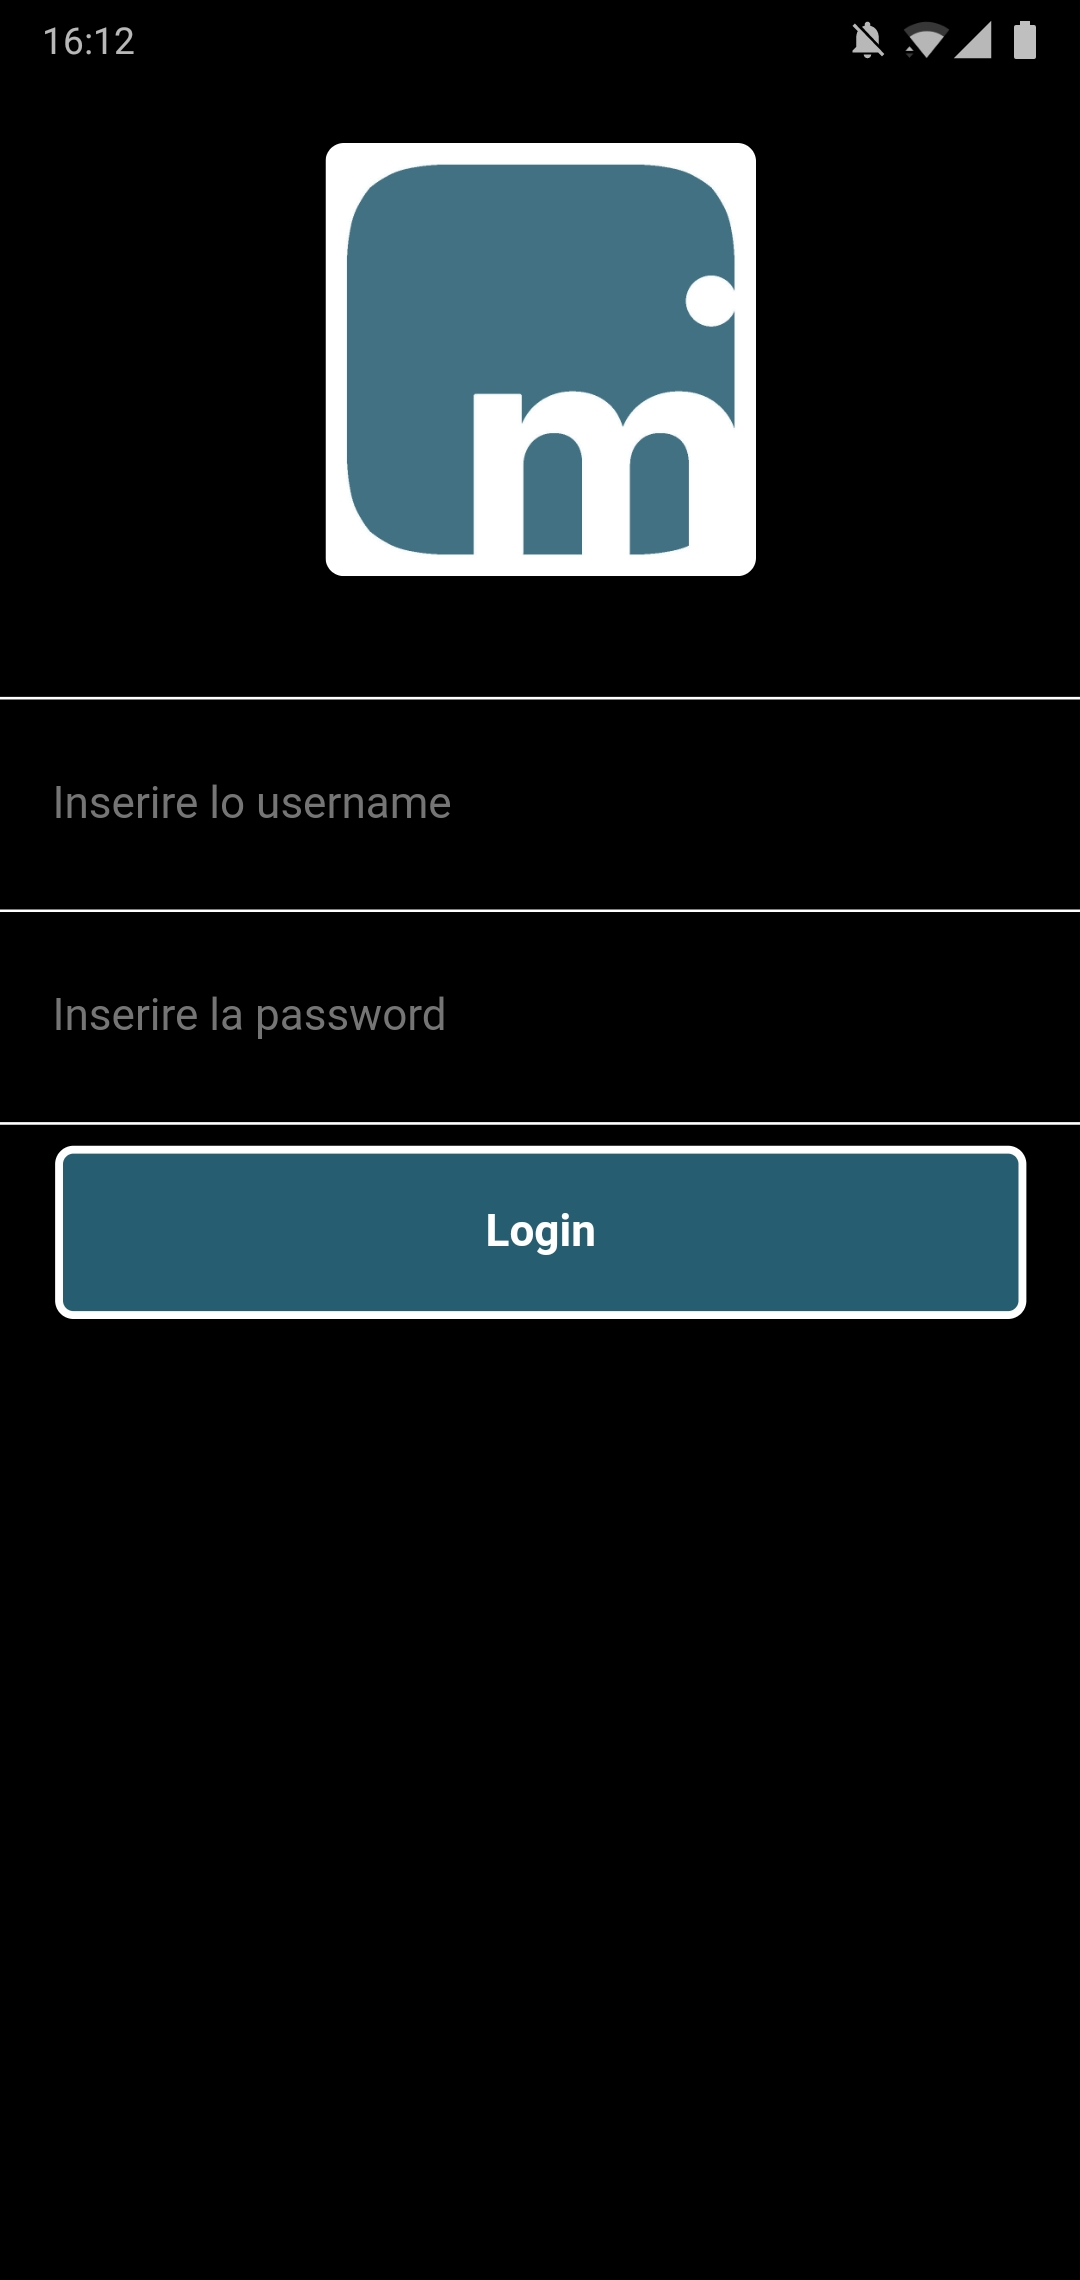
\includegraphics[width=.3\textwidth]{./img/login.jpg}
	\caption{Pagina di login}
\end{figure}

La pagina di login è costituita dalle seguenti quattro parti, a partire dall'alto verso il basso:
\begin{itemize}
	\item \textbf{Logo}: è il logo di moviORDER;
	\item \textbf{Input box username}: è l'input box per l'inserimento dello username. Quando la pagina viene aperta, viene consigliato di inserire lo 		username;
	\item \textbf{Input box password}: è l'input box per l'inserimento della password. Quando la pagina viene aperta, viene consigliato di inserire la 		password;
	\item \textbf{Pulsante di Login}: è il pulsante per tentare l'accesso all'app. Se il pulsante viene premuto, viene tentato l'accesso a moviORDER con i dati inseriti nella form.
\end{itemize}

In base ai dati inseriti nella form e ai dati di accesso presenti sul server cloud di VISIONEIMPRESA, possono avvenire quattro casistiche:
\begin{enumerate}
	\item \textbf{Nome utente non corretto}: sul server cloud non è presente il nome utente inserito. Potrebbe essere stato inserito non correttamente
	o potrebbe essere che l'azienda fornitrice non abbia ancora fornito i dati di accesso a VISIONEIMPRESA;
	\item \textbf{Password non corretta}: sul server cloud è presente il nome utente inserito, ma la password ad esso associata è diversa da quella
	inserita. Potrebbe essere stata inserita non correttamente oppure l'azienda potrebbe aver cambiato la password e non averla ancora inviata
	a VISIONEIMPRESA;
	\item \textbf{Username e password non inserite}: se il bottone viene premuto senza inserire lo username e/o la password, viene visualizzato un
	messaggio che notifica all'utente l'errore commesso;
	\item \textbf{Dati corretti}: se il pulsante viene premuto e i dati sono corretti, l'applicazione aprirà la home page.
\end{enumerate}

\begin{figure}[h]

\centering
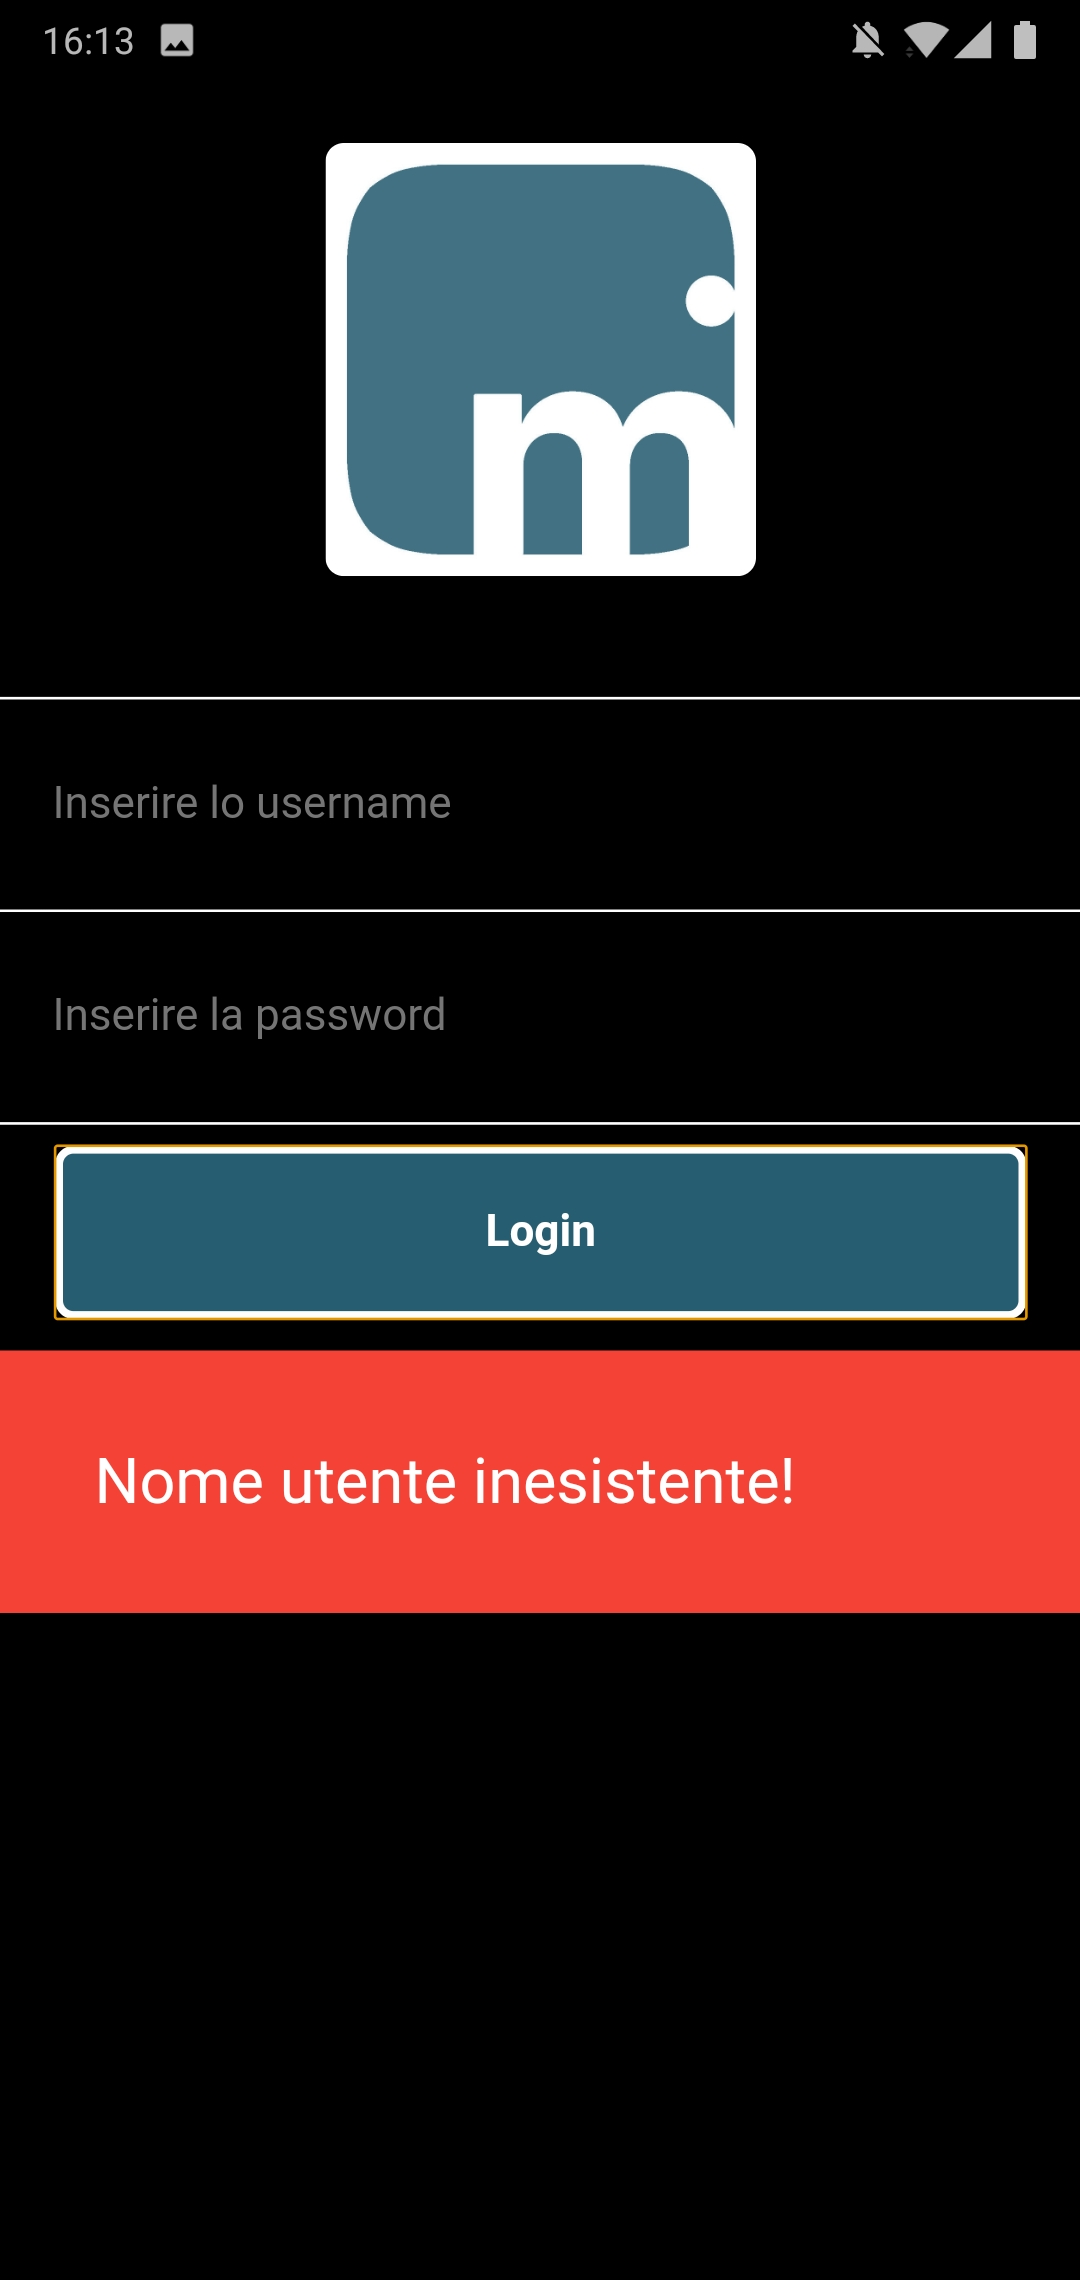
\includegraphics[width=.3\textwidth]{./img/erroreUsr.jpg}\hfill
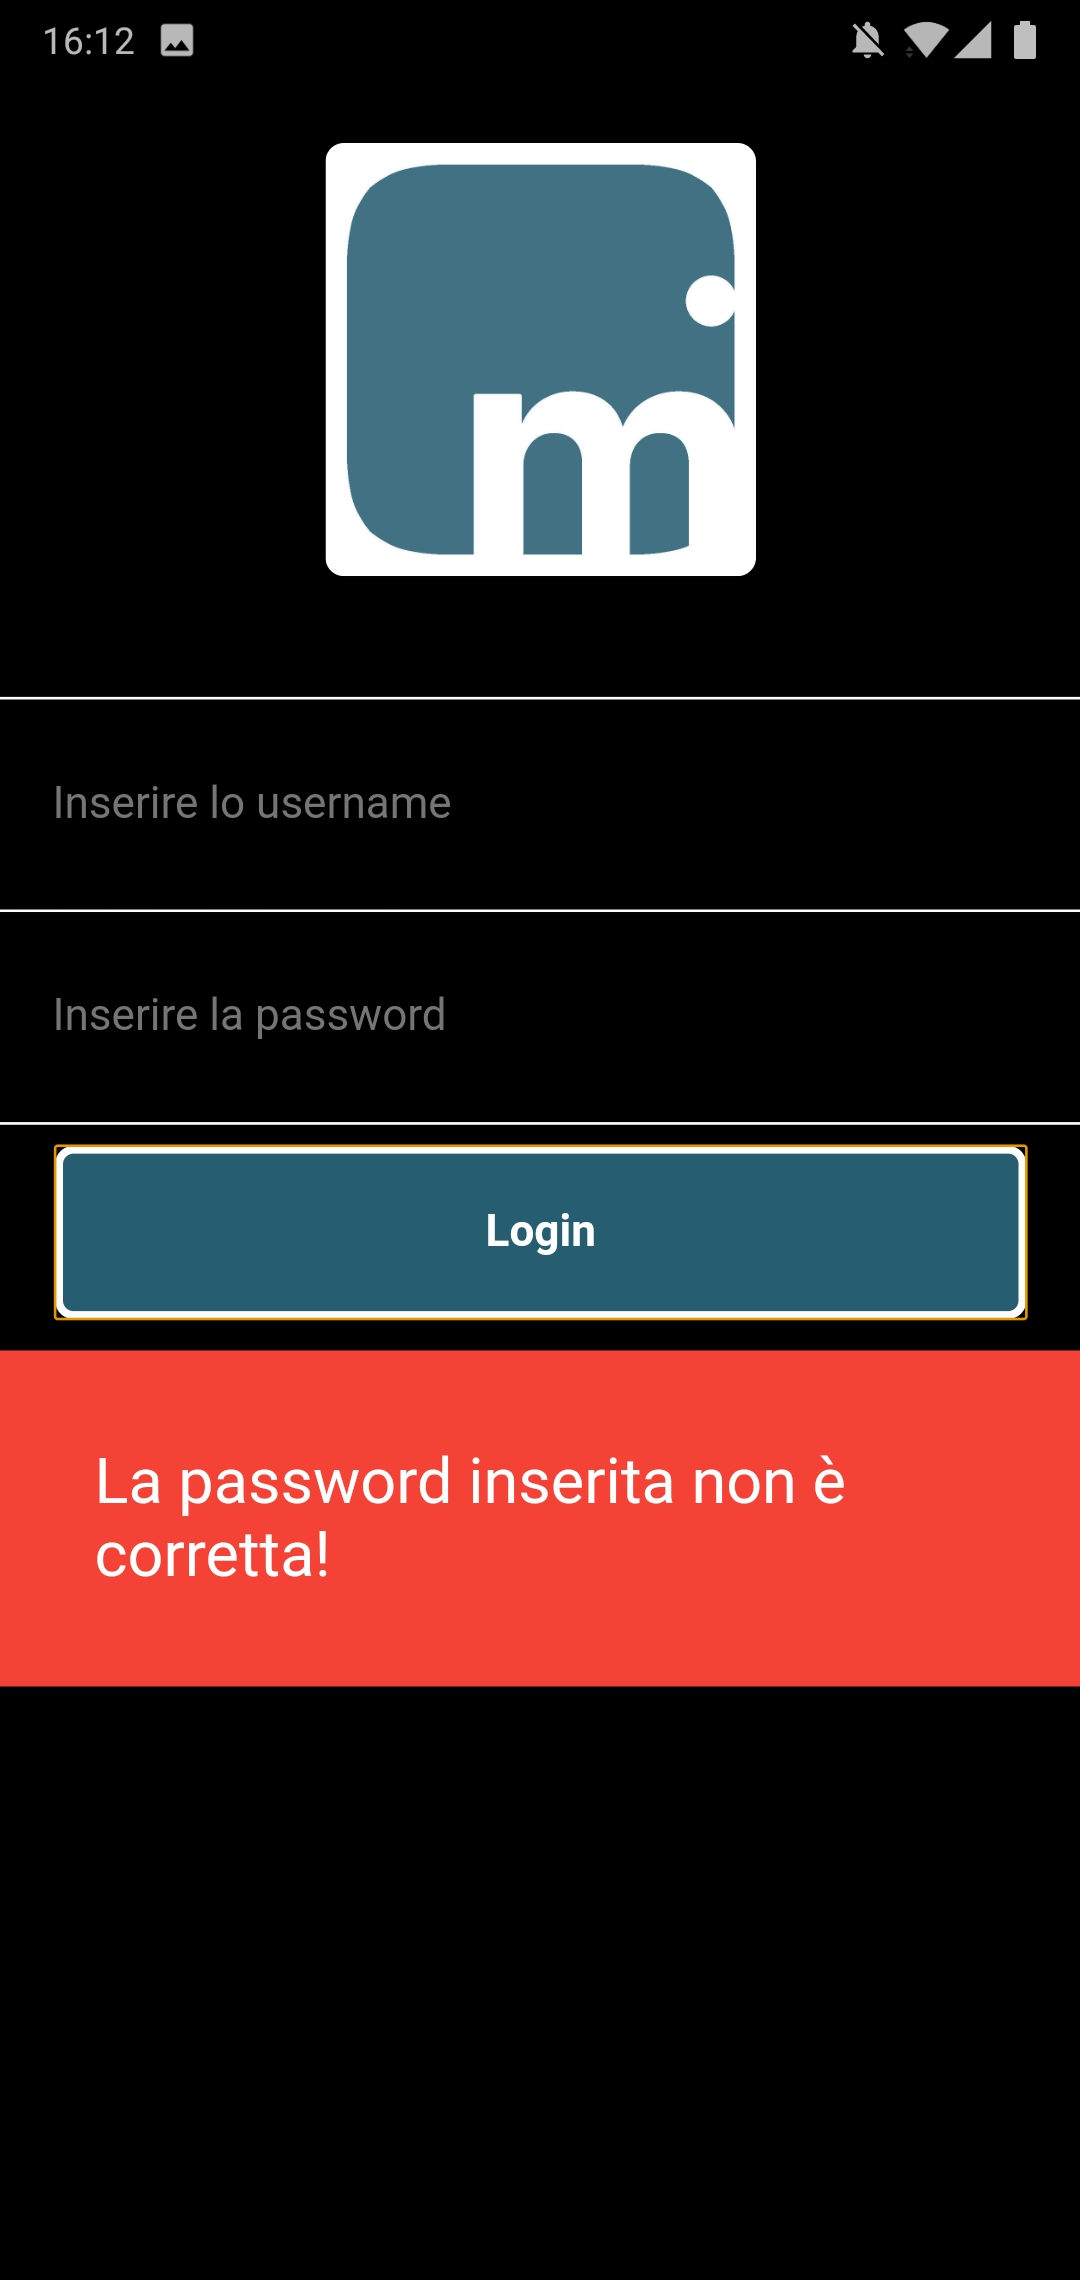
\includegraphics[width=.3\textwidth]{./img/errorePwd.jpg}\hfill
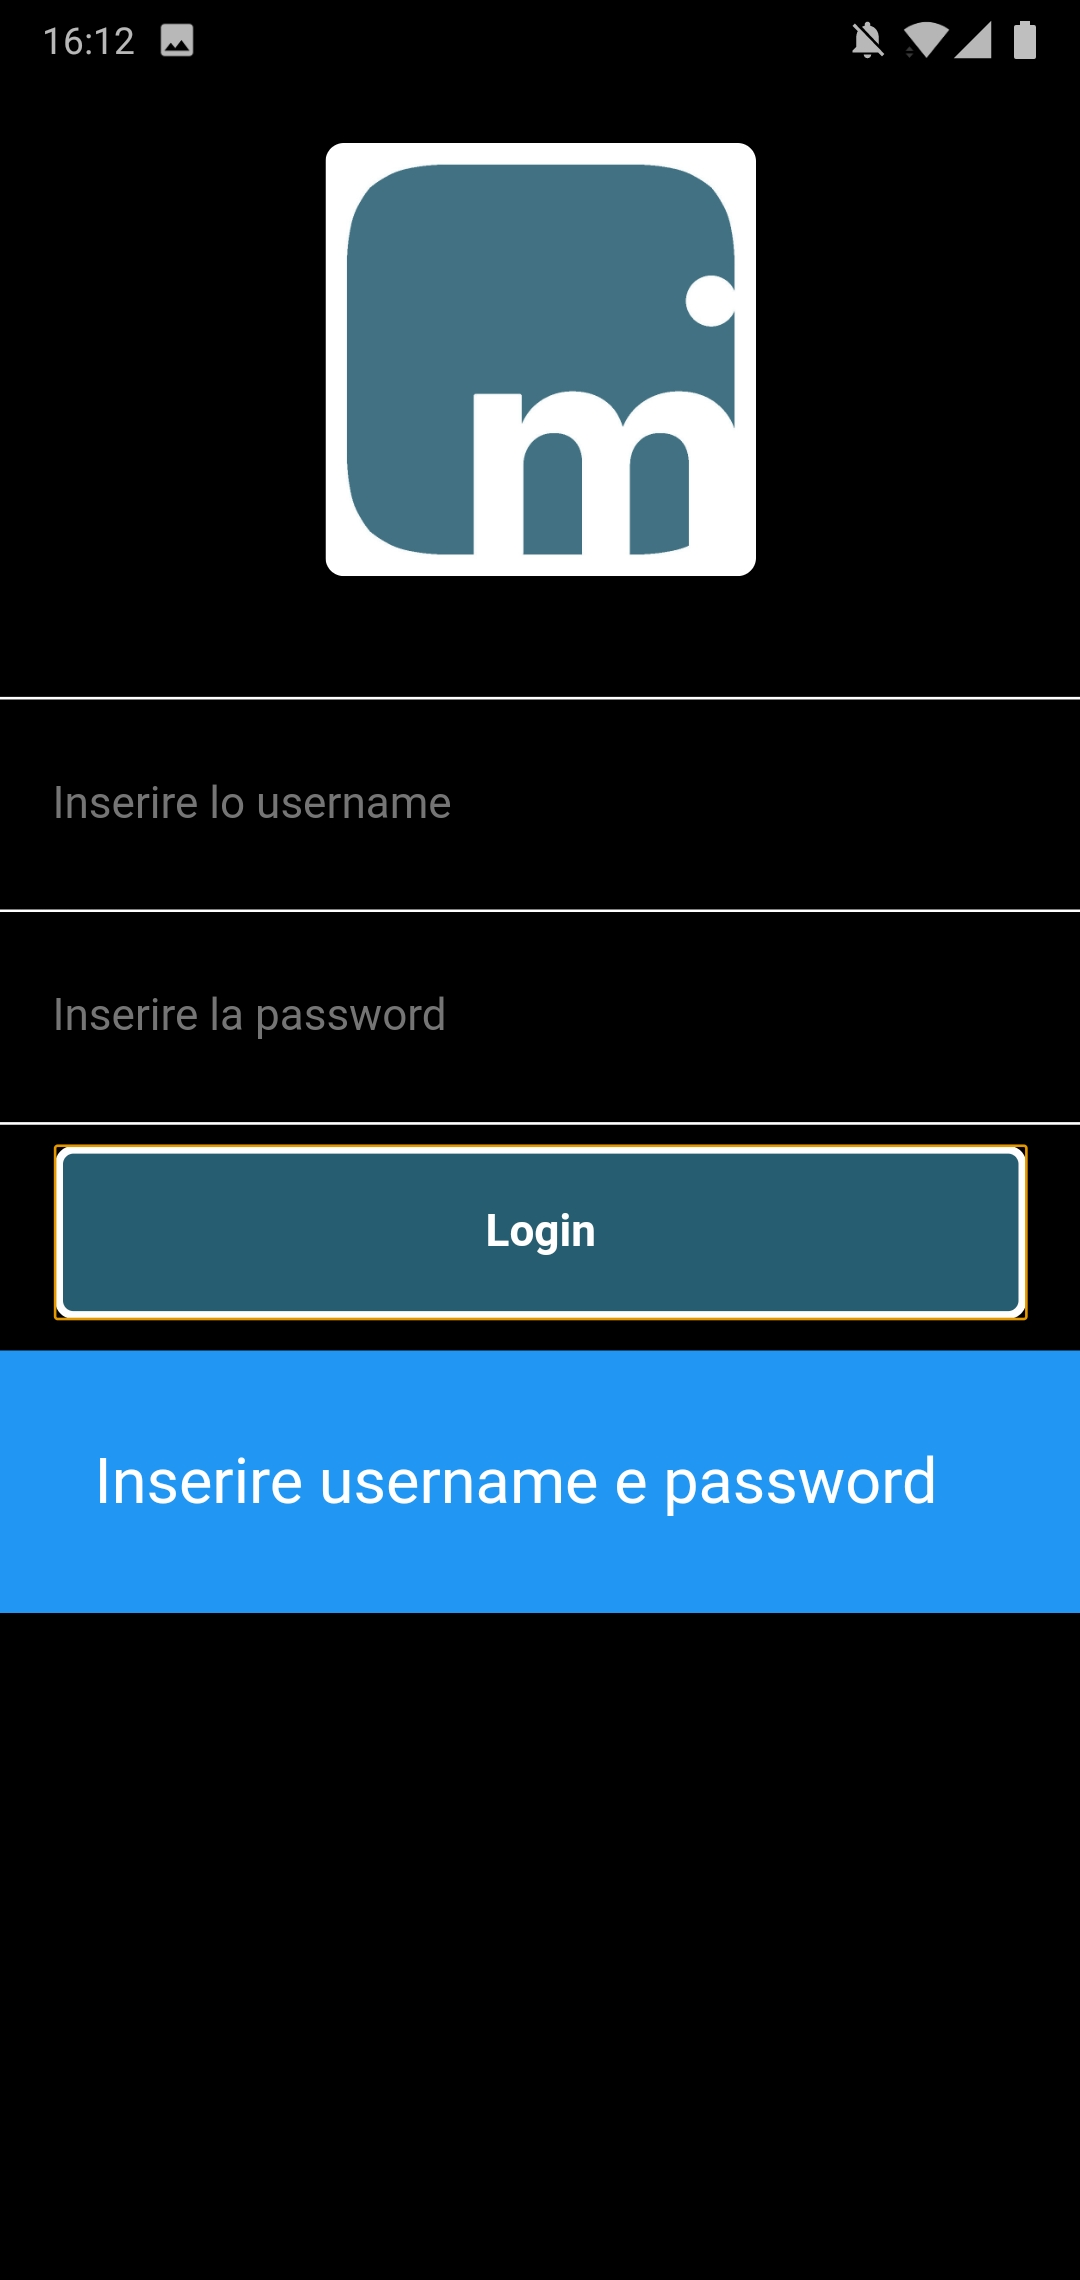
\includegraphics[width=.3\textwidth]{./img/erroreIns.jpg}

\caption{Possibili messaggi dell'applicazione in fase di login}

\end{figure}

\newpage

\subsection{Pagina principale}

\begin{figure}[h]
	\centering
	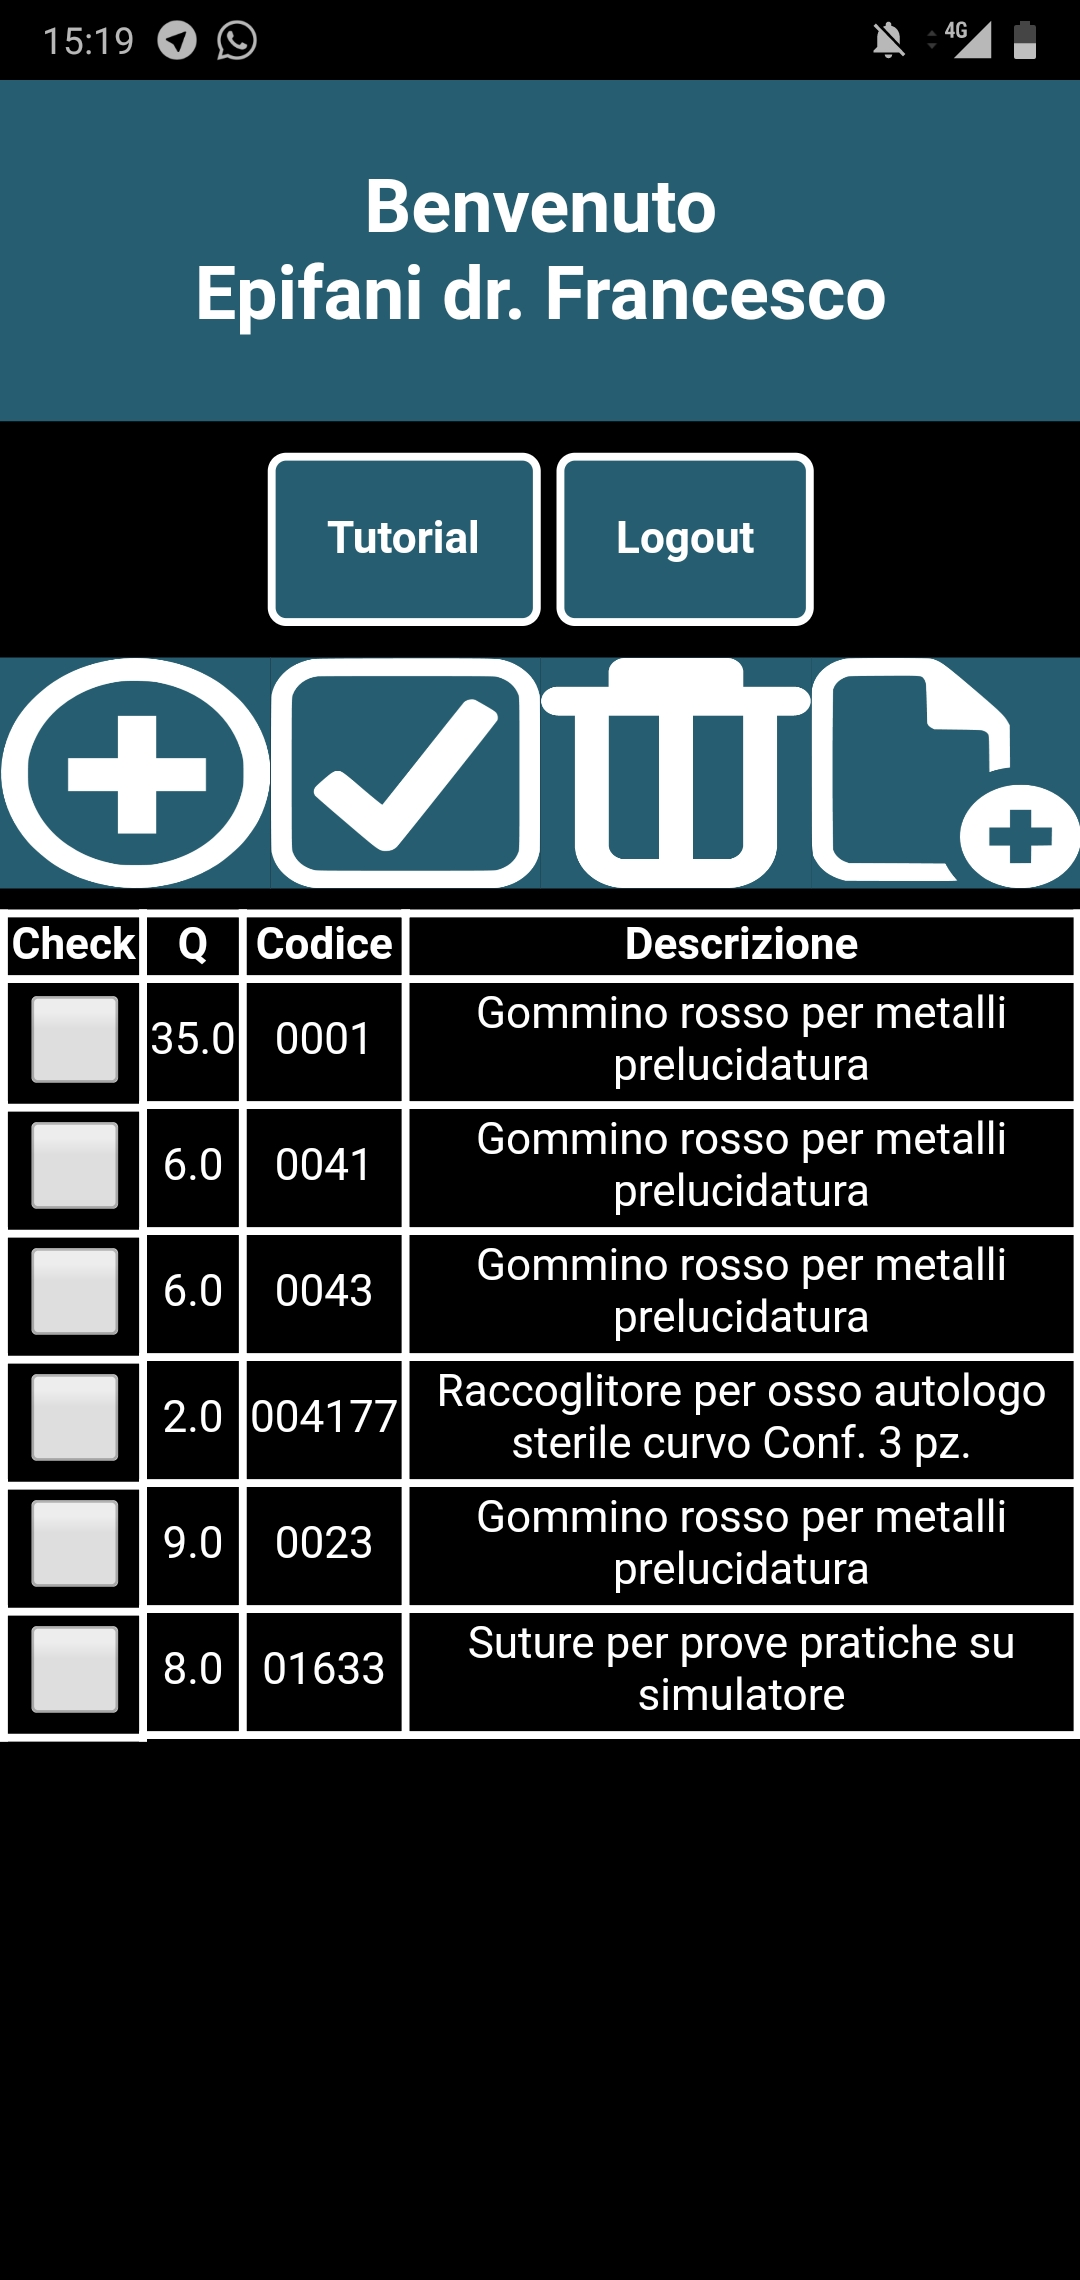
\includegraphics[width=.3\textwidth]{./img/homepage.jpg}
	\caption{Pagina principale}
\end{figure}

La pagina principale è composta dalle seguenti quattro parti, a partire dall'alto verso il basso:
\begin{itemize}
	\item \textbf{Testata}: contiene un messaggio di benvenuto per l'utente che si è appena loggato. Il messaggio contiene il nome dell'utente;
	\item \textbf{Pulsanti}: contiene due pulsanti:
	\begin{itemize}
		\item \textbf{Tutorial}: pulsante che permette di visualizzare un breve tutorial dell'applicazione. Se premuto, il tutorial viene 
		visualizzato tramite un dialog;
		\item \textbf{Logout}: pulsante che permette di effettuare il logout dall'applicazione. Il logout consiste nell'uscire dalla pagina
		principale per tornare alla pagina di login.
	\end{itemize}
	\item \textbf{Pulsanti gestione carrello}: contiene 4 pulsanti utili alla gestione del carrello. Essi sono descritti nella sezione sottostante §\ref{gestione};
	\item \textbf{Tabella carrello}: contiene una tabella contenente tutti gli articoli che l'utente loggato ha in carrello. Per ogni articolo vi è una riga in tabella con le seguenti componenti:
	\begin{enumerate}
		\item \textbf{Check-box}: check-box per selezionare/deselezionare un articolo per l'inserimento in ordine o la cancellazione;
		\item \textbf{Quantità}: contiene la quantità di pezzi che si vogliono ordinare dell'articolo;
		\item \textbf{Codice}: contiene il codice univoco dell'articolo;
		\item \textbf{Descrizione}: contiene un nome che descrive l'articolo.
	\end{enumerate}
\end{itemize}

Infine, se l'utente loggato non ha articoli in carrello, viene visualizzato un messaggio che lo specifica.

\begin{figure}[h]
	\centering
	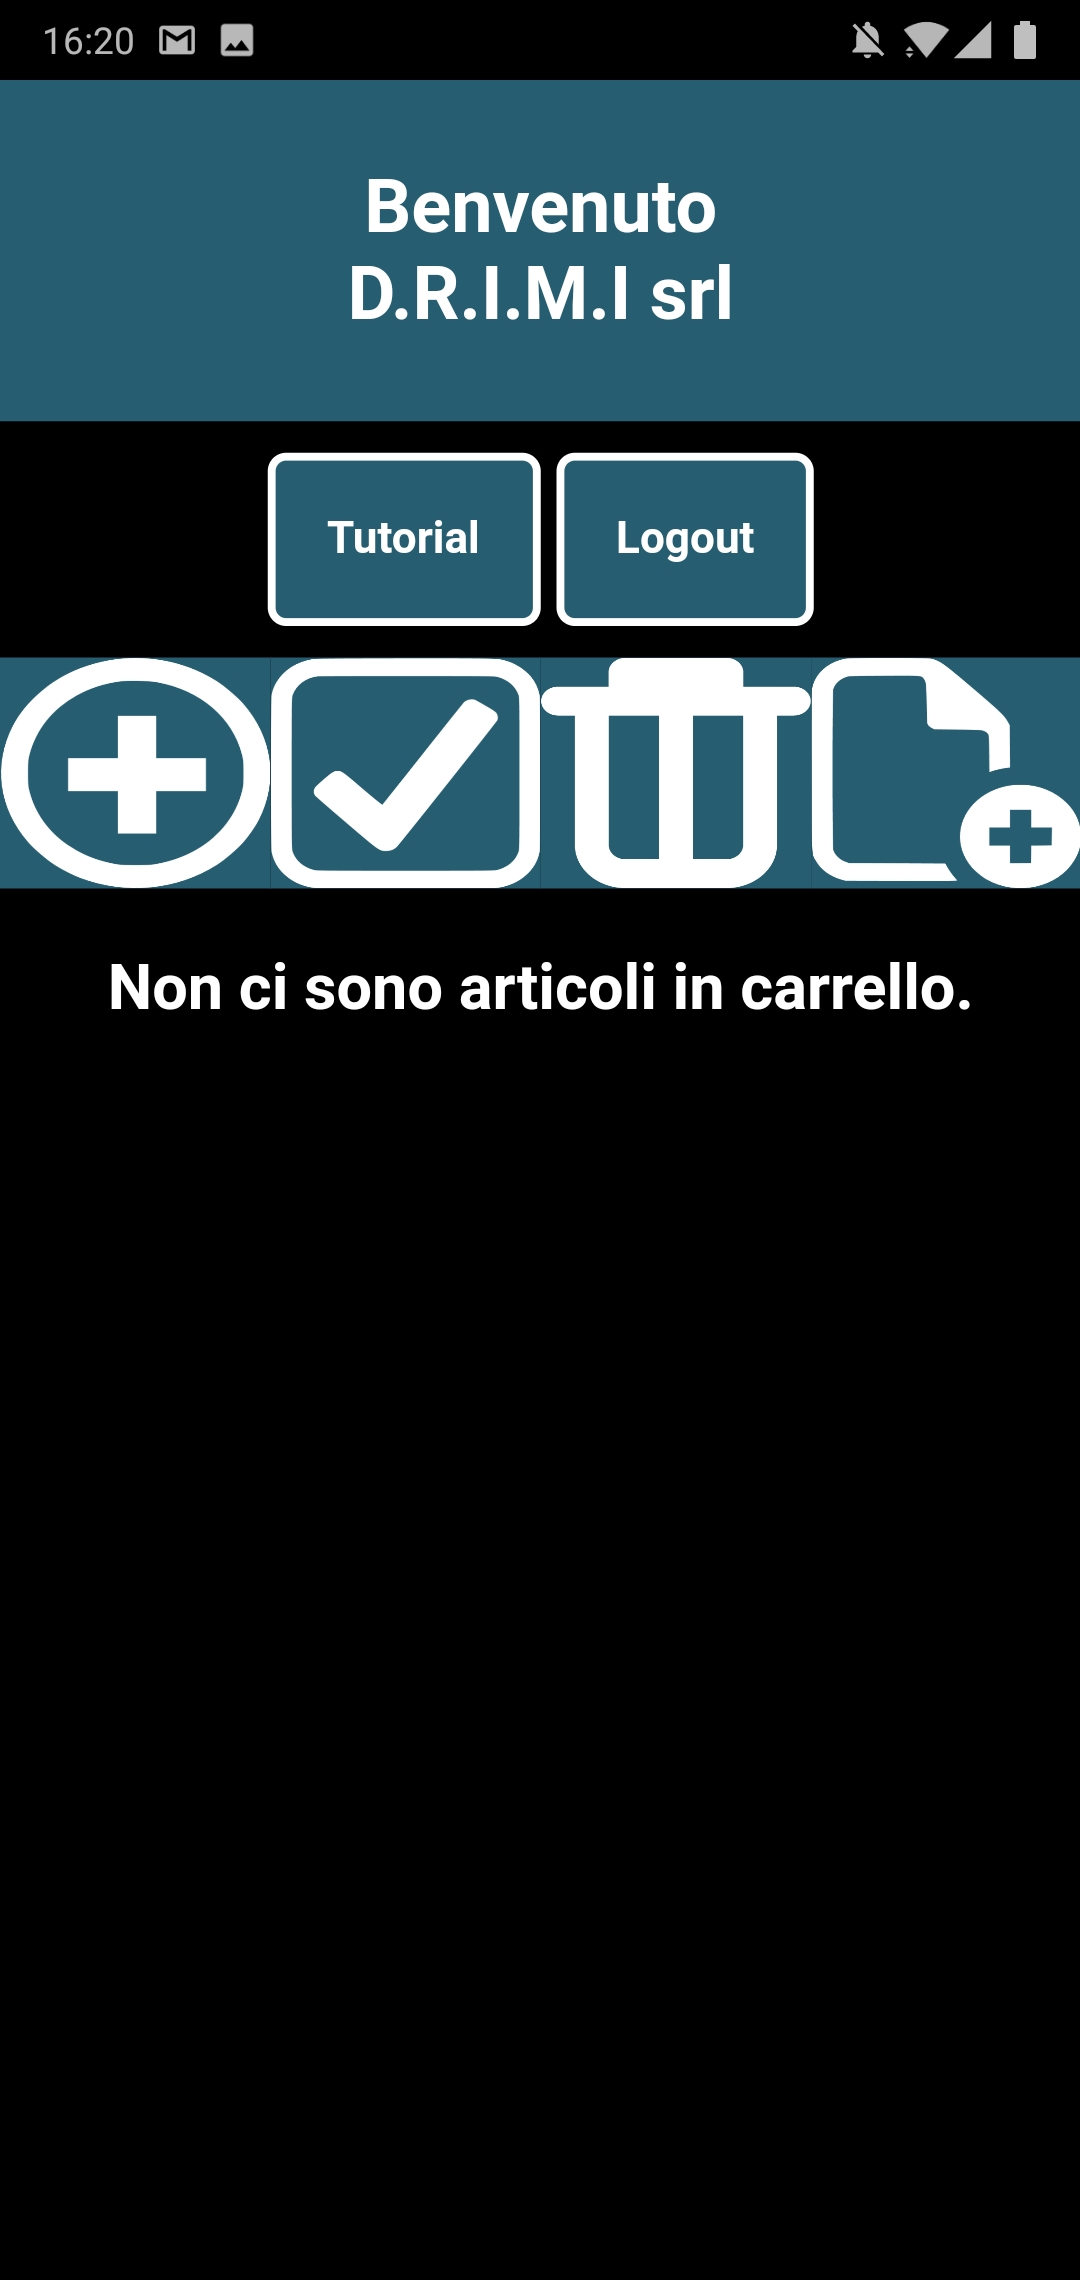
\includegraphics[width=.3\textwidth]{./img/vuoto.jpg}
	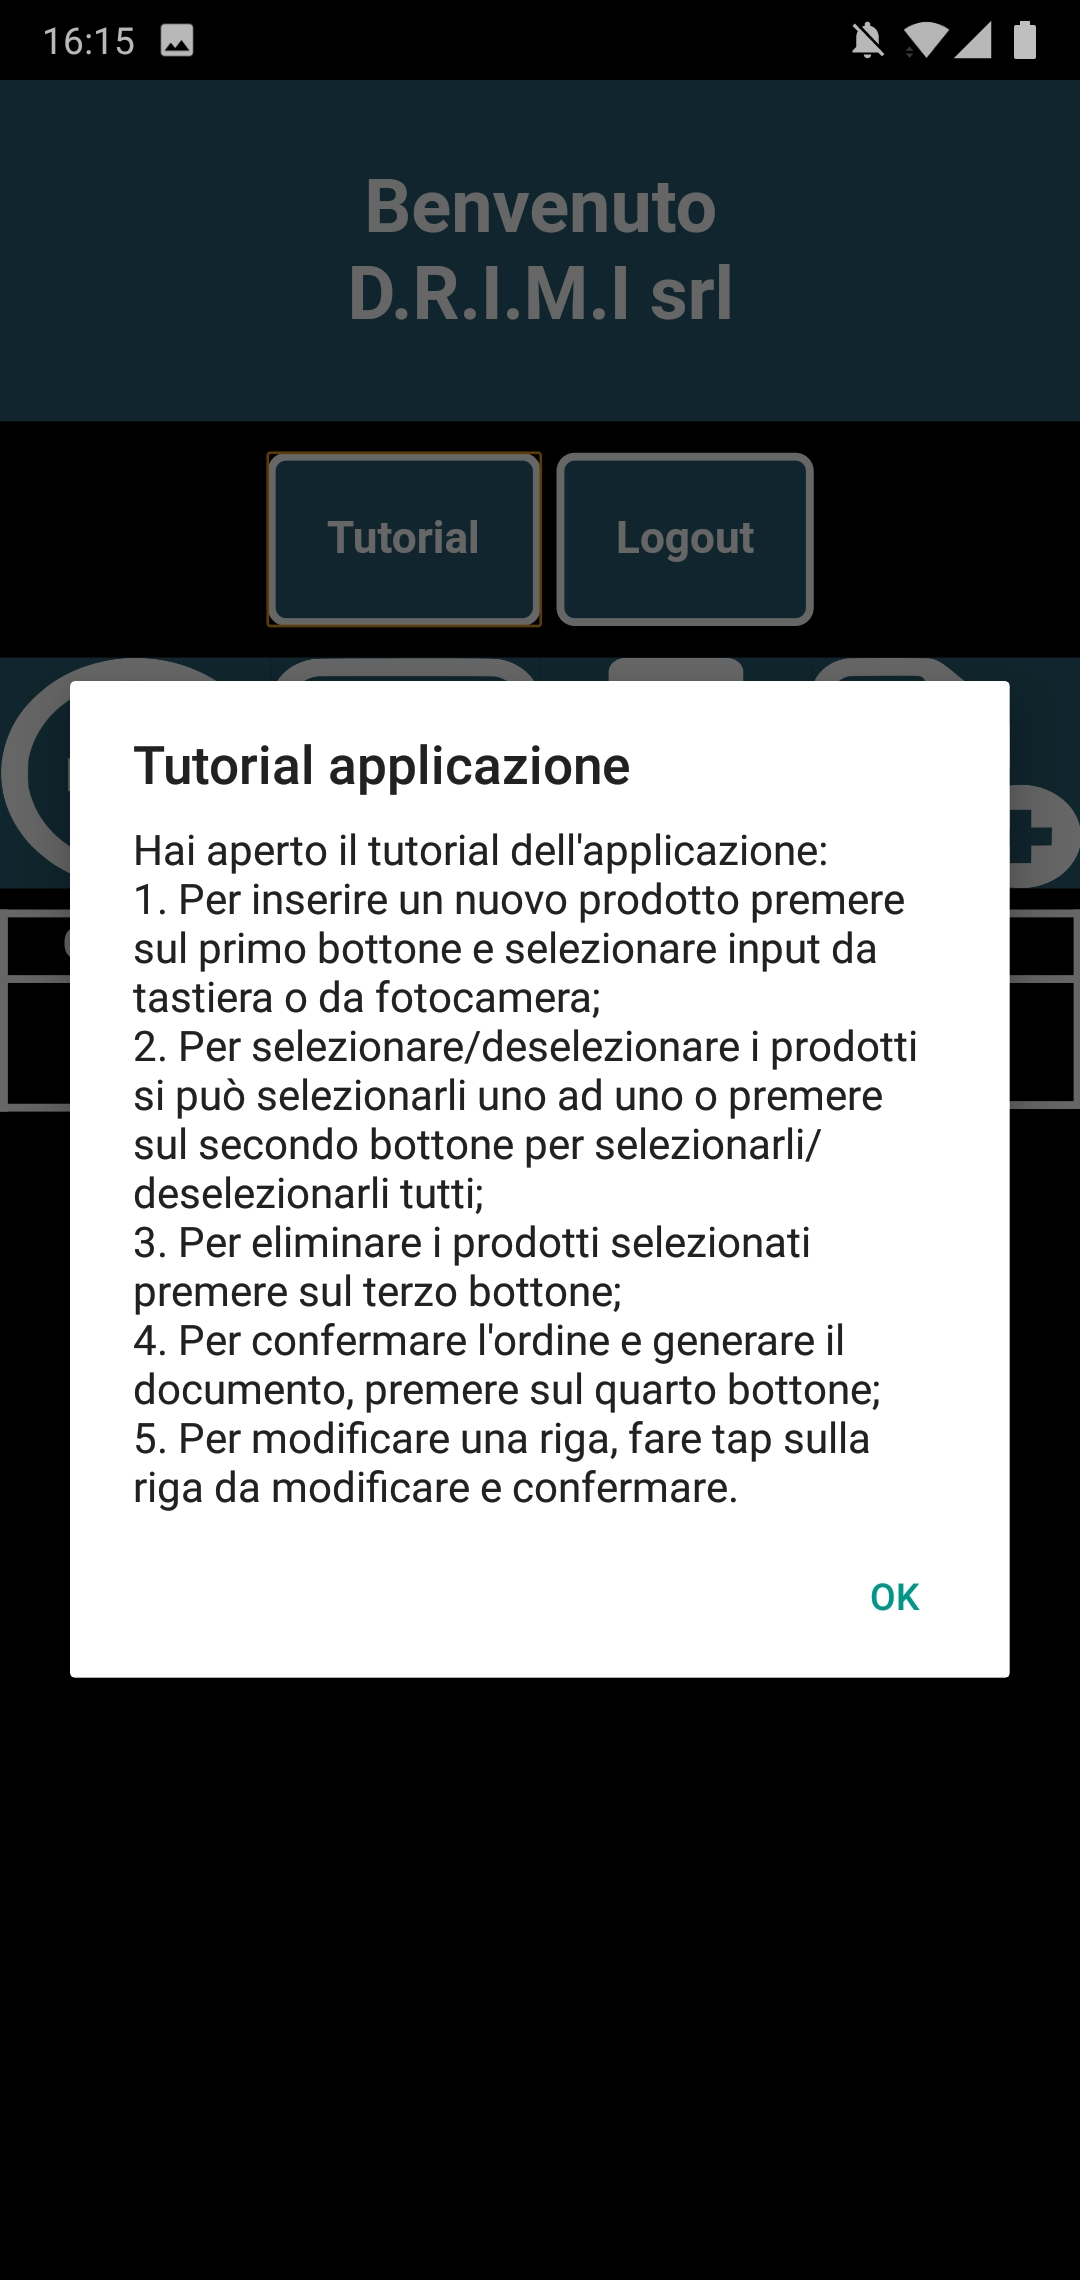
\includegraphics[width=.3\textwidth]{./img/tutorial.jpg}
	\caption[Possibili dialog sulla home page]{A sinistra il caso di carrello vuoto; a destra il dialog che mostra il tutorial dell'applicazione}
\end{figure}
\newpage

\subsubsection{Pulsanti di gestione del carrello} \label{gestione}

I pulsanti sono illustrati a partire da sinistra andando verso destra.
\begin{table}[h]
	\centering
	\begin{tabular}{| c | >{\arraybackslash}m{14cm} |}
		\hline
		\textbf{Pulsante} & \textbf{Funzione} \\ \hline
		
\includegraphics[]{./img/add.png} & Pulsante che permette di aggiungere un nuovo articolo in carrello. La procedura di aggiunta di 
		un articolo è spiegata in sezione §\ref{add}. \\ \hline
		
\includegraphics[]{./img/select.png} & Pulsante che permette di selezionare/deselezionare tutti gli articoli in carrello. Se ci sono già degli articoli selezionati, seleziona anche tutti i restanti articoli. \\ \hline
		
\includegraphics[]{./img/cestino.png} & Pulsante che permette di eliminare gli articoli selezionati. La procedura di cancellazione di
		un articolo è spiegata in sezione §\ref{remove}.  \\ \hline
		
\includegraphics[]{./img/nuovoDocumento.png} & Pulsante che permette di creare un nuovo ordine con gli articoli selezionati. La procedura di creazione di un nuovo ordine è spiegata in sezione §\ref{new}. \\ \hline
 	\end{tabular}
 	\caption{Tabella dei pulsanti per la gestione del carrello}
\end{table}

\newpage

\myparagraph{Aggiunta di un articolo} \label{add}

\begin{figure}[h]
	\centering
	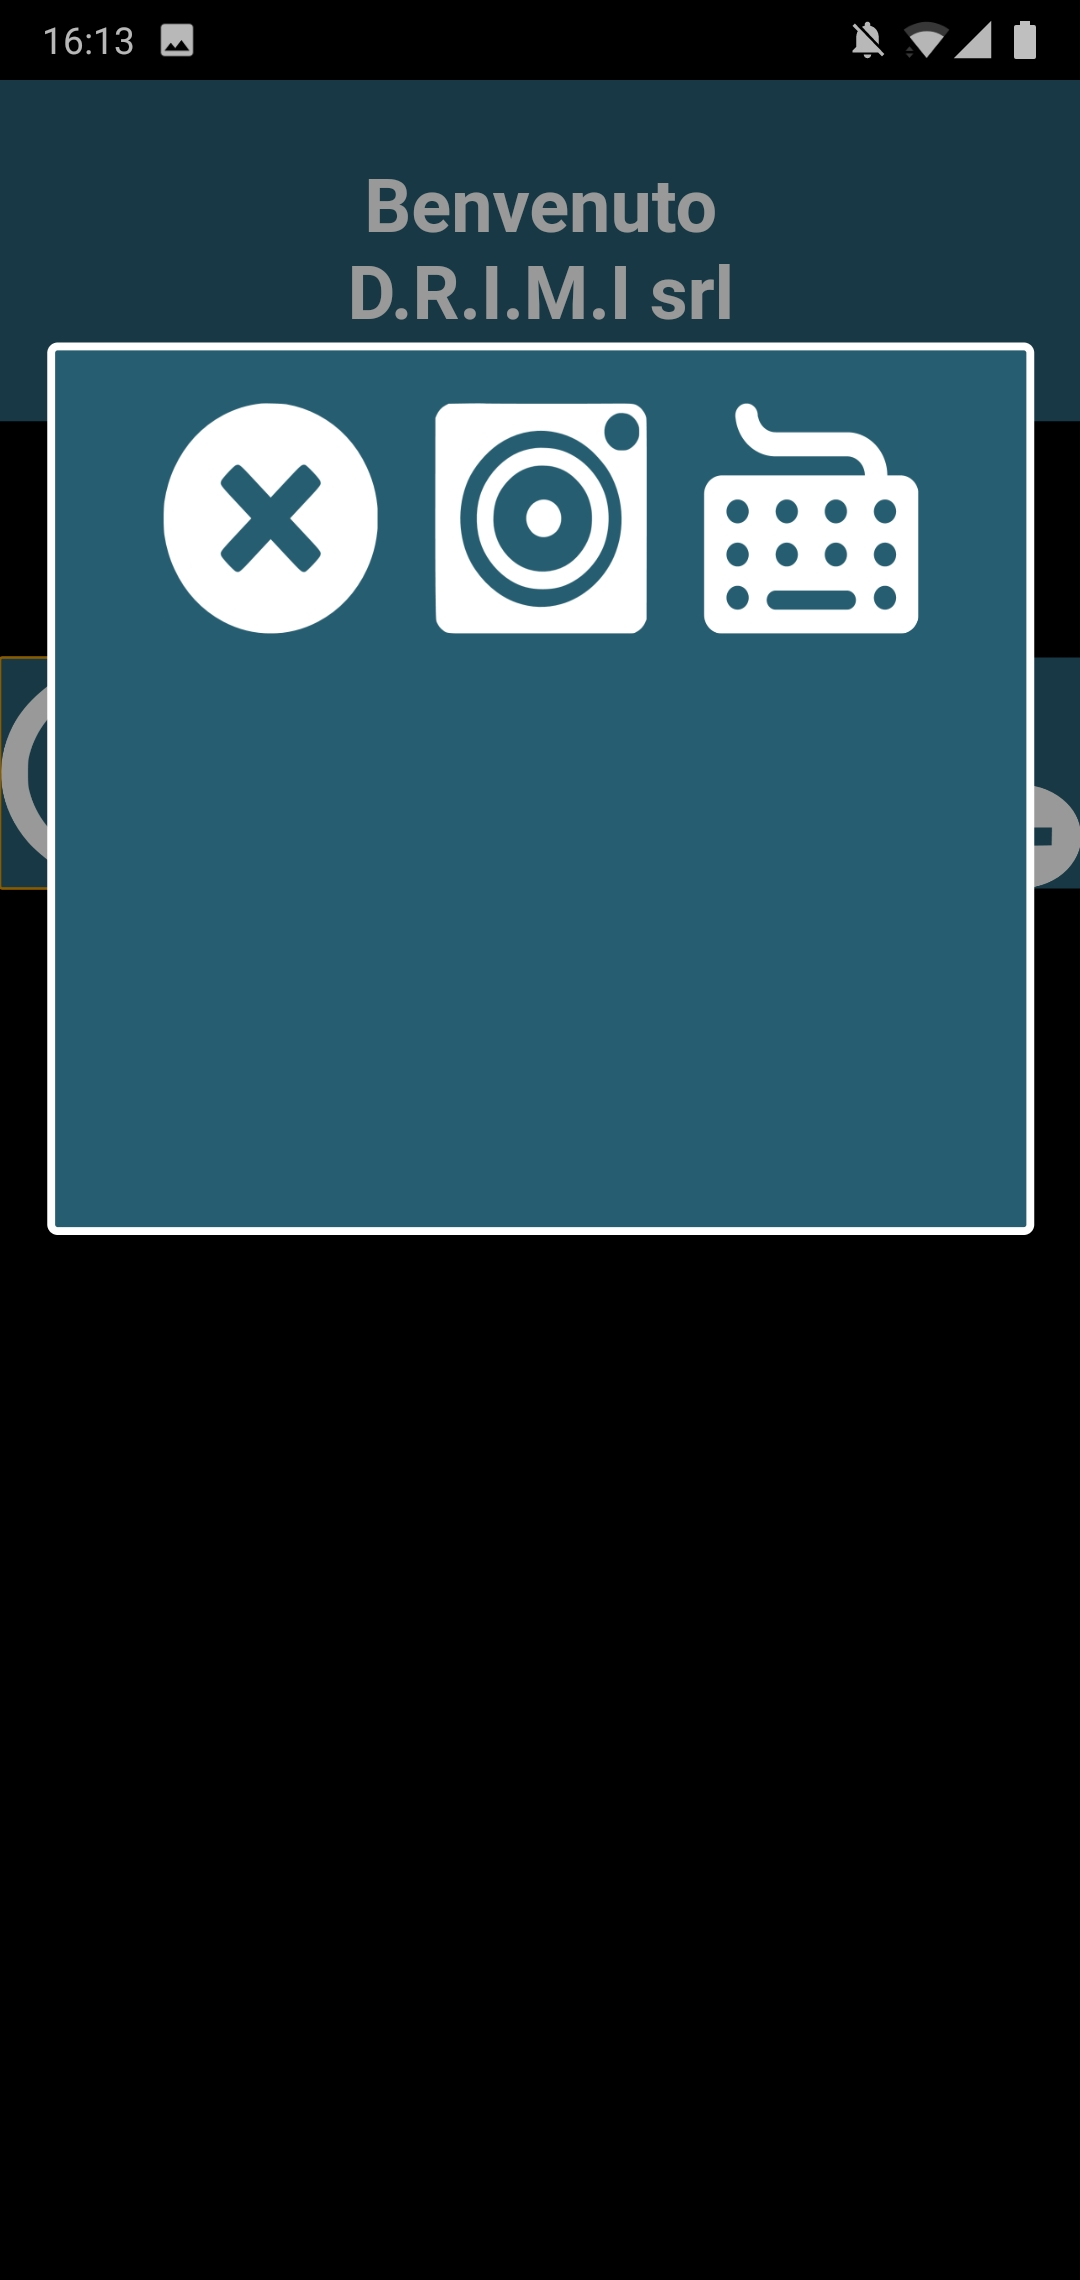
\includegraphics[width=.3\textwidth]{./img/modal.jpg}\hfill
	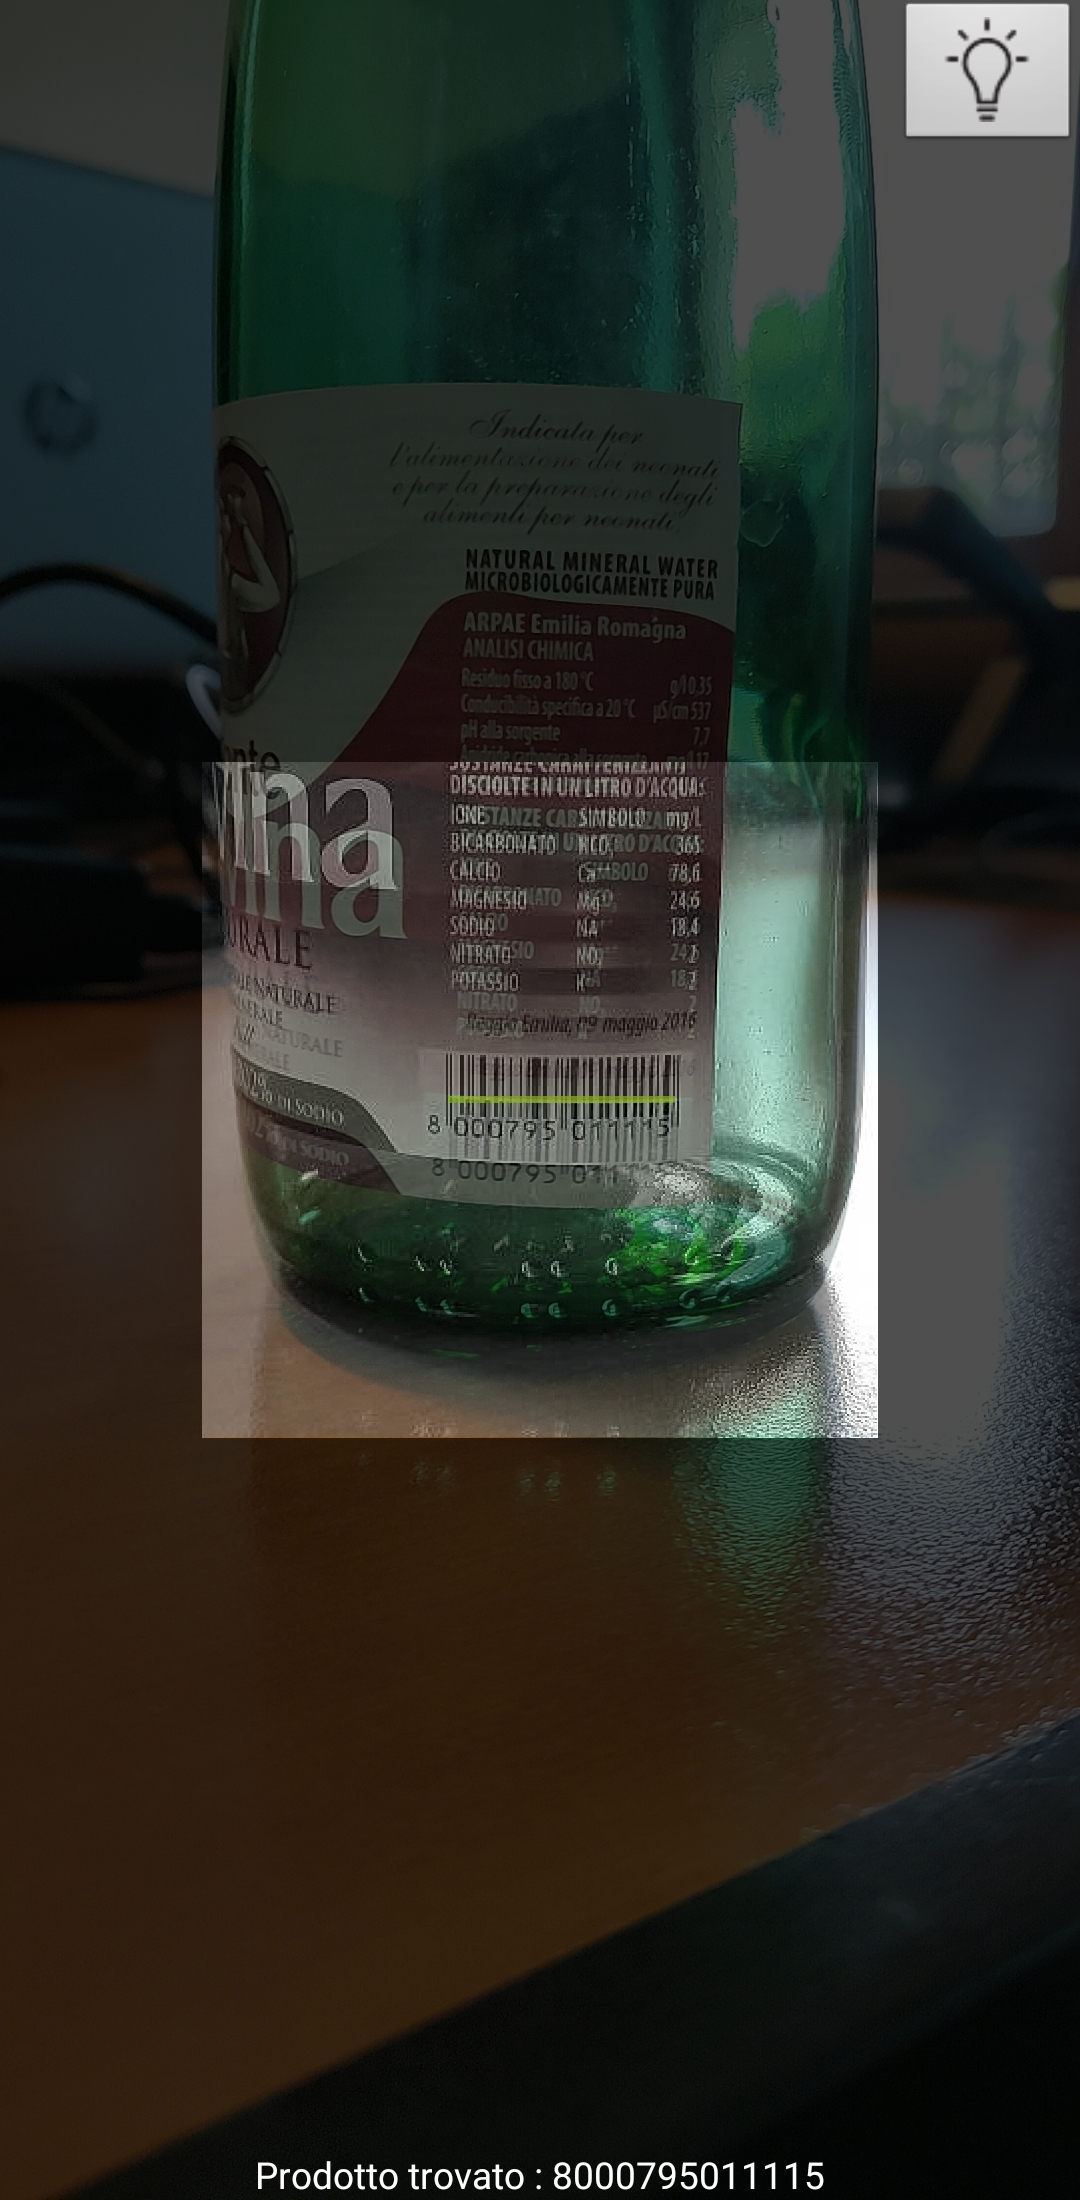
\includegraphics[width=.3\textwidth]{./img/scan.jpg}\hfill
	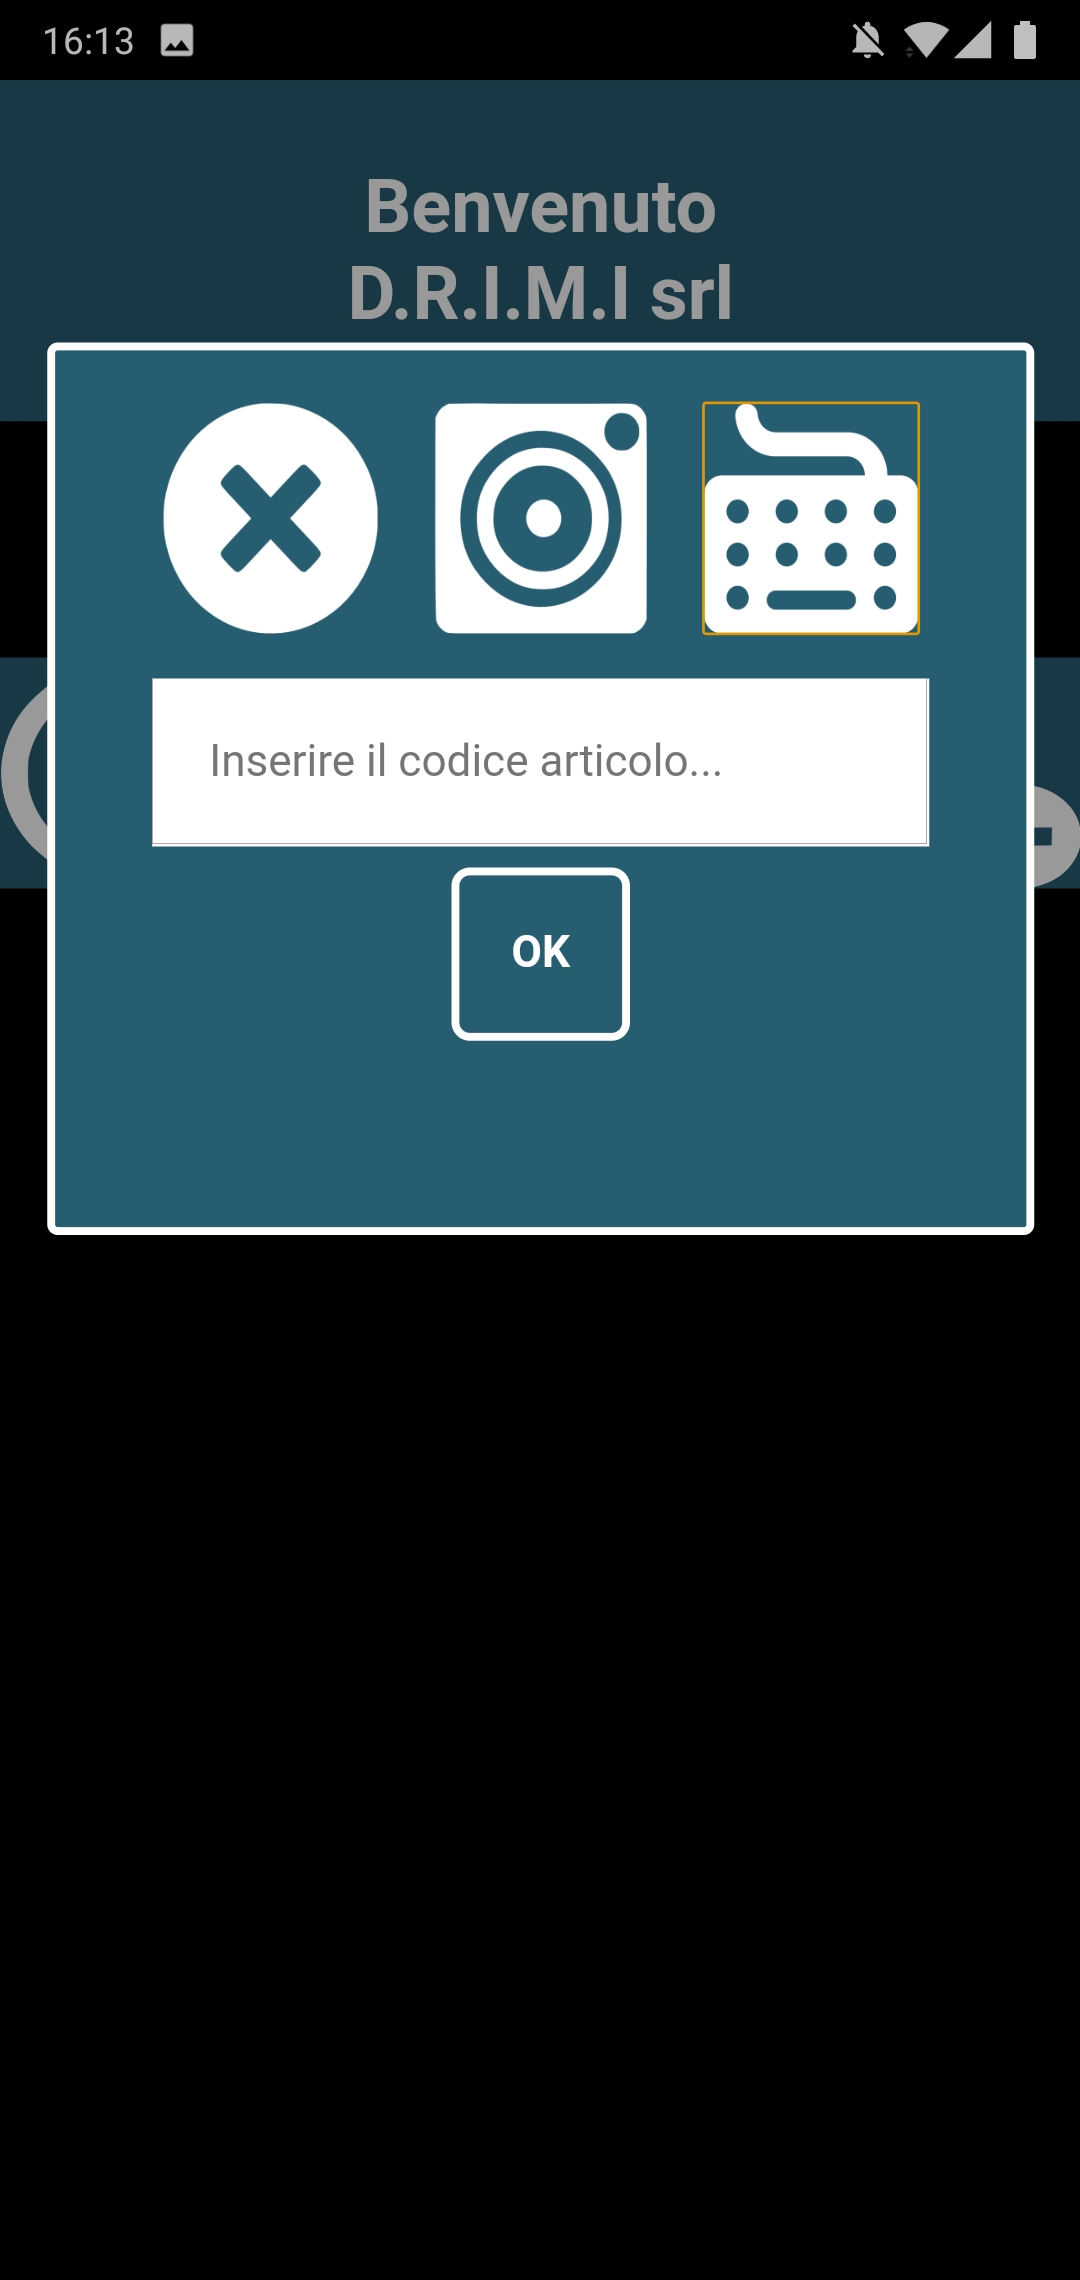
\includegraphics[width=.3\textwidth]{./img/modalInput.jpg}
	\caption{Modal di inserimento di un nuovo articolo}
\end{figure}

La procedura di aggiunta di un articolo consiste nel:
\begin{enumerate}
	\item Premere il pulsante di aggiunta di un articolo;
	\item Selezionare una modalità tra le due possibili, fotocamera o tastierino, nel modal che viene aperto successivamente:
		\begin{enumerate}
			\item Inserimento articolo tramite scansione di un codice a barre con la fotocamera: verrà aperta una pagina con una preview
			della fotocamera, con un riquadro verde al centro dove deve essere centrato il codice a barre da scansionare. Se il pulsante viene
			premuto per la prima volta, viene richiesto il permesso per l'utilizzo della fotocamera da parte del dispositivo;
			\item Inserimento articolo tramite digitazione del codice articolo.
		\end{enumerate}
\end{enumerate}

Nel caso in cui sia stata scelta la modalità fotocamera, il suo funzionamento è diverso a seconda del sistema operativo del dispositivo:
\begin{itemize}
	\item \textbf{Android}: nel momento in cui l'app rileva un codice a barre, verrà visualizzata un'animazione;
	\item \textbf{IoS}: nel momento in cui l'app rileva un codice a barre, verrà emesso un suono acustico.
\end{itemize}

\newpage

Tutti i casi possibili durante la scansione del codice a barre sono i seguenti:
\begin{enumerate}
	\item La scansione del codice a barre va a \textbf{buon fine}: verrà aperta la pagina per l'inserimento del nuovo articolo. La pagina viene aperta
	solamente se l'articolo non è già presente in carrello. In tal caso viene visualizzato un messaggio informativo che invita l'utente
	a modificarne la quantità direttamente dal carrello;
	\item La scansione del codice a barre \textbf{non va a buon fine}: verrà visualizzato con un dialog con un messaggio d'errore. L'errore può
	essere di due tipologie:
		\begin{itemize}
			\item Codice a barre \textbf{non corrispondente ad un articolo venduto} dal fornitore: nel caso in cui l'utente ha scansionato un articolo
			che non fa parte di quelli venduti dal fornitore;
			\item Codice a barre scansionato in maniera \textbf{non corretta} dallo scanner: l'utente potrebbe aver messo l'articolo in una posizione
			in cui il codice a barre è risultato complesso da captare.
		\end{itemize}
	\item La scansione del codice a barre viene \textbf{cancellata} dall'utente: l'utente può cancellare la scansione premendo il pulsante indietro. In
	questo caso, con un dialog box, viene visualizzato un messaggio informativo per notificare la cancellazione della scansione.
\end{enumerate}

\begin{figure}[h]

\centering
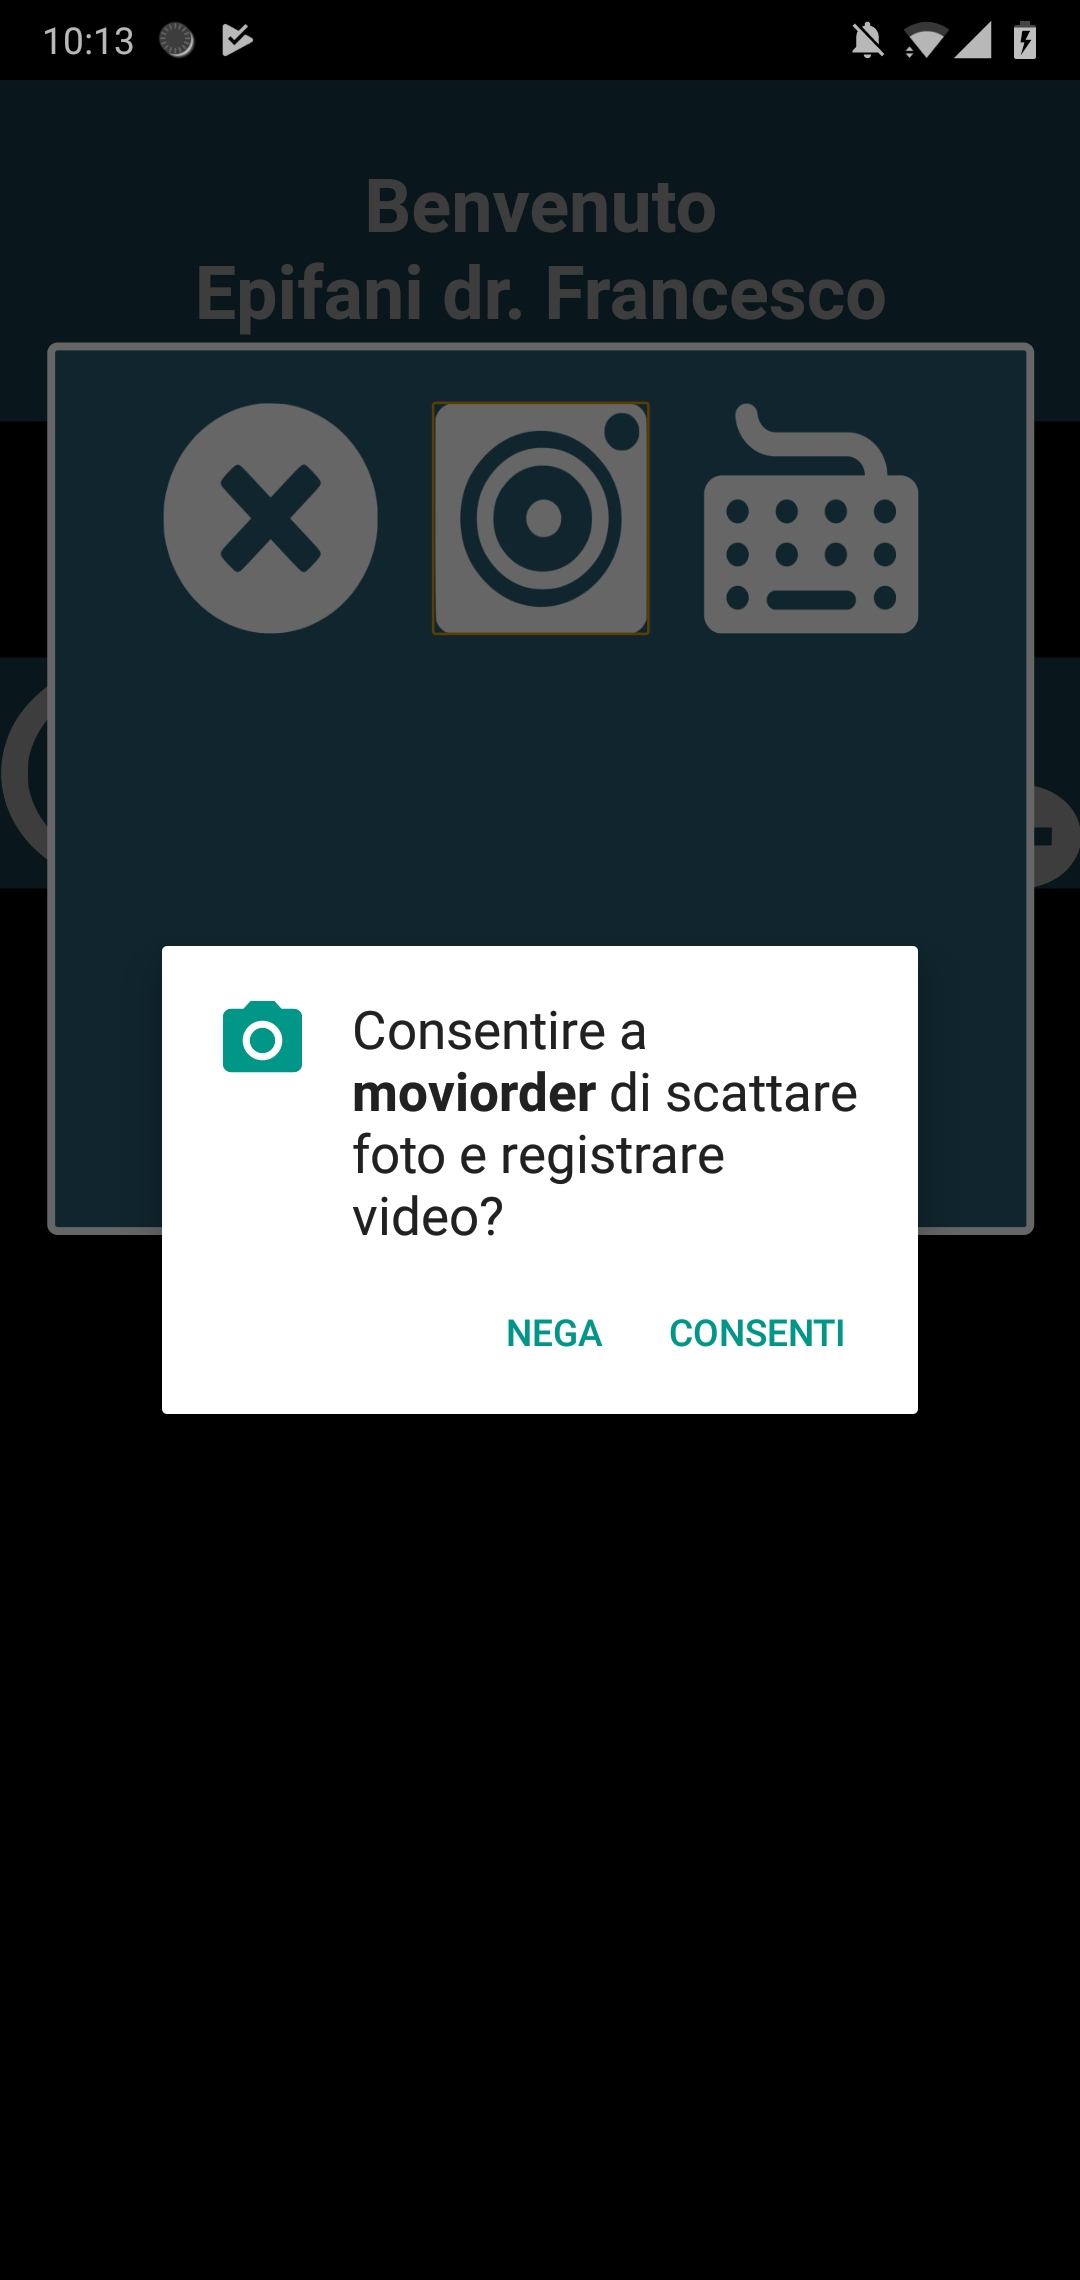
\includegraphics[width=.3\textwidth]{./img/permesso.jpg}\hfill
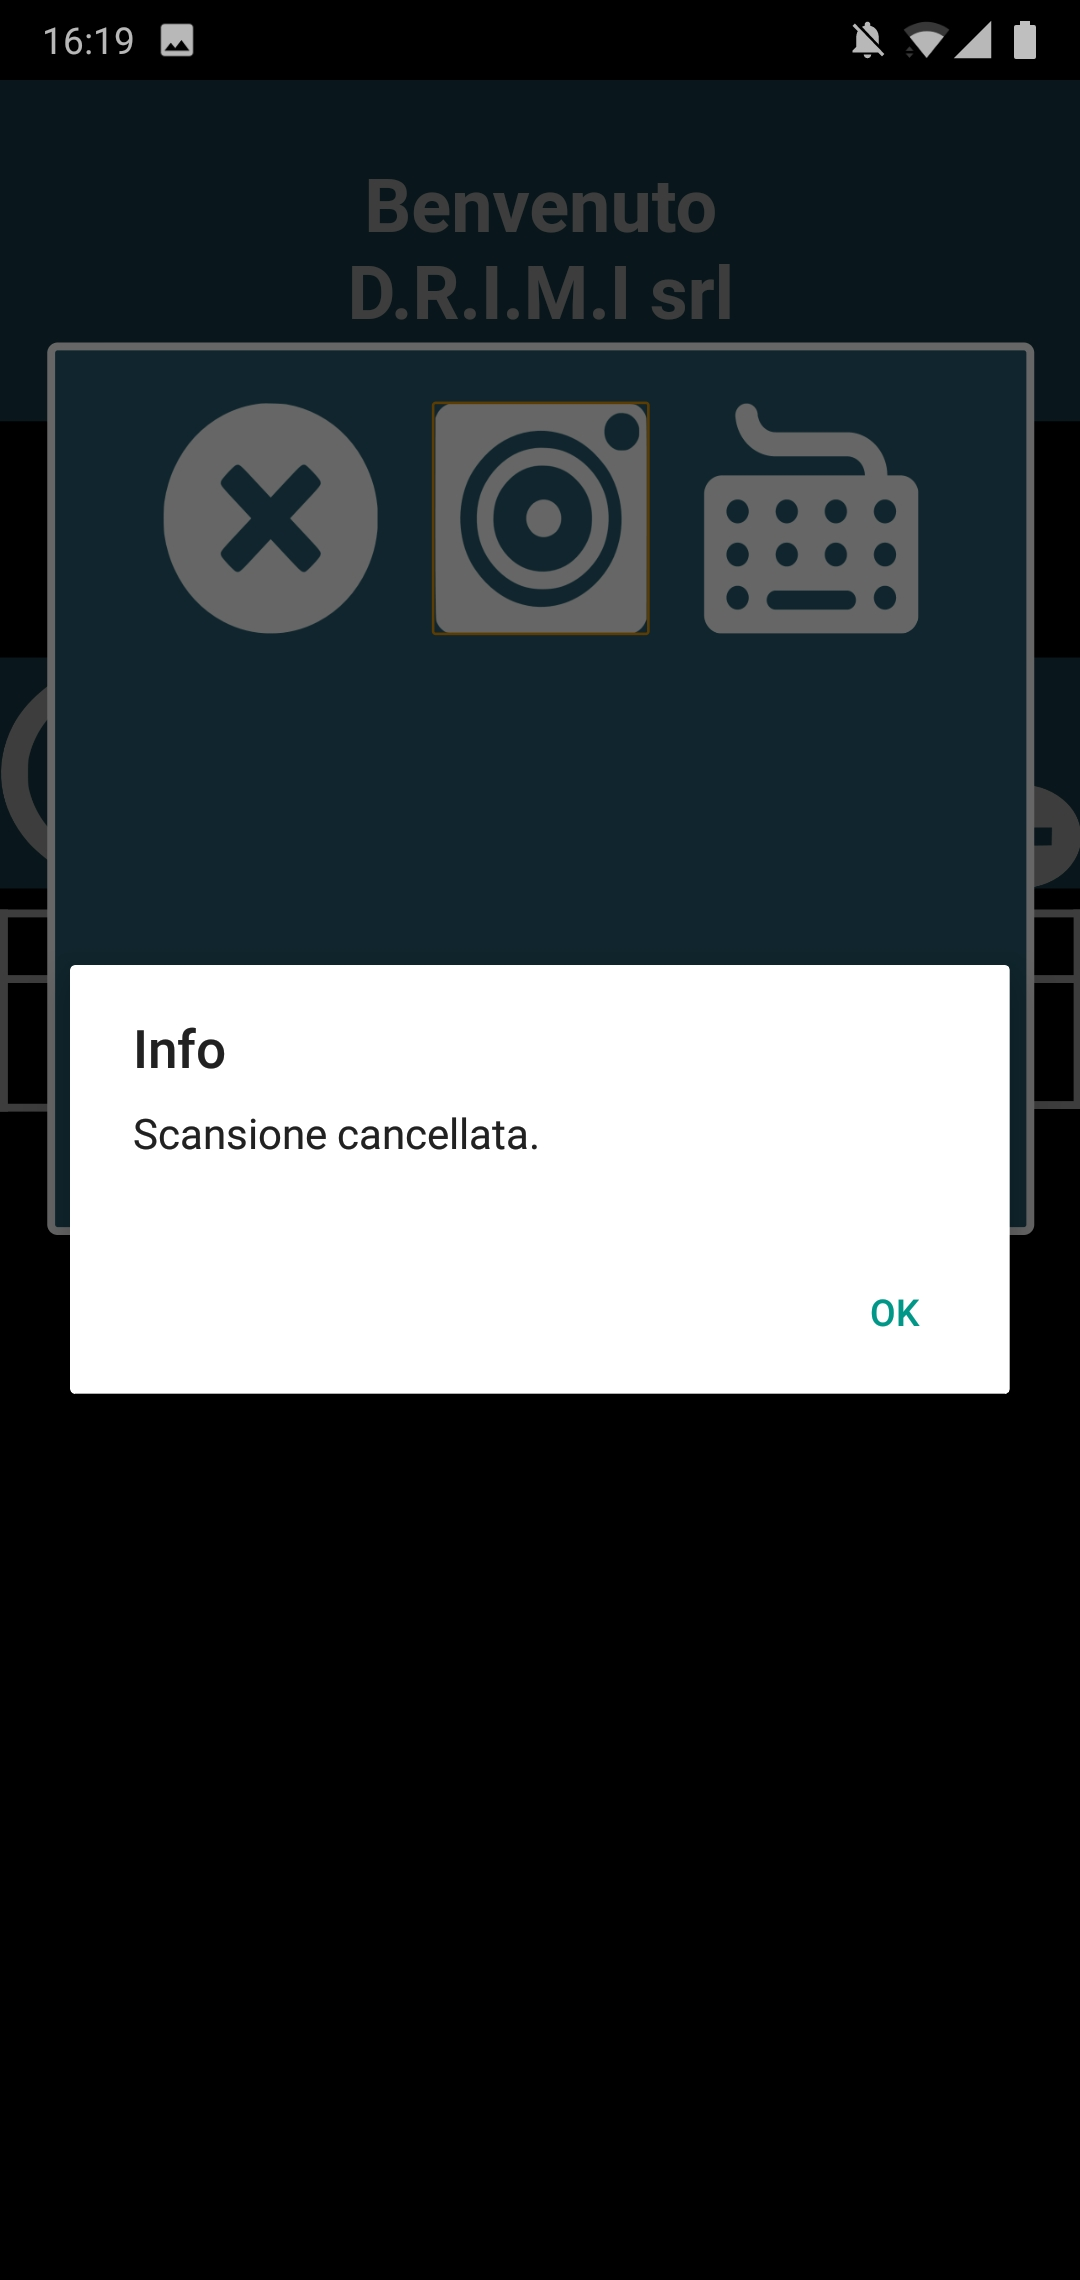
\includegraphics[width=.3\textwidth]{./img/erroreScanCanc.jpg}\hfill
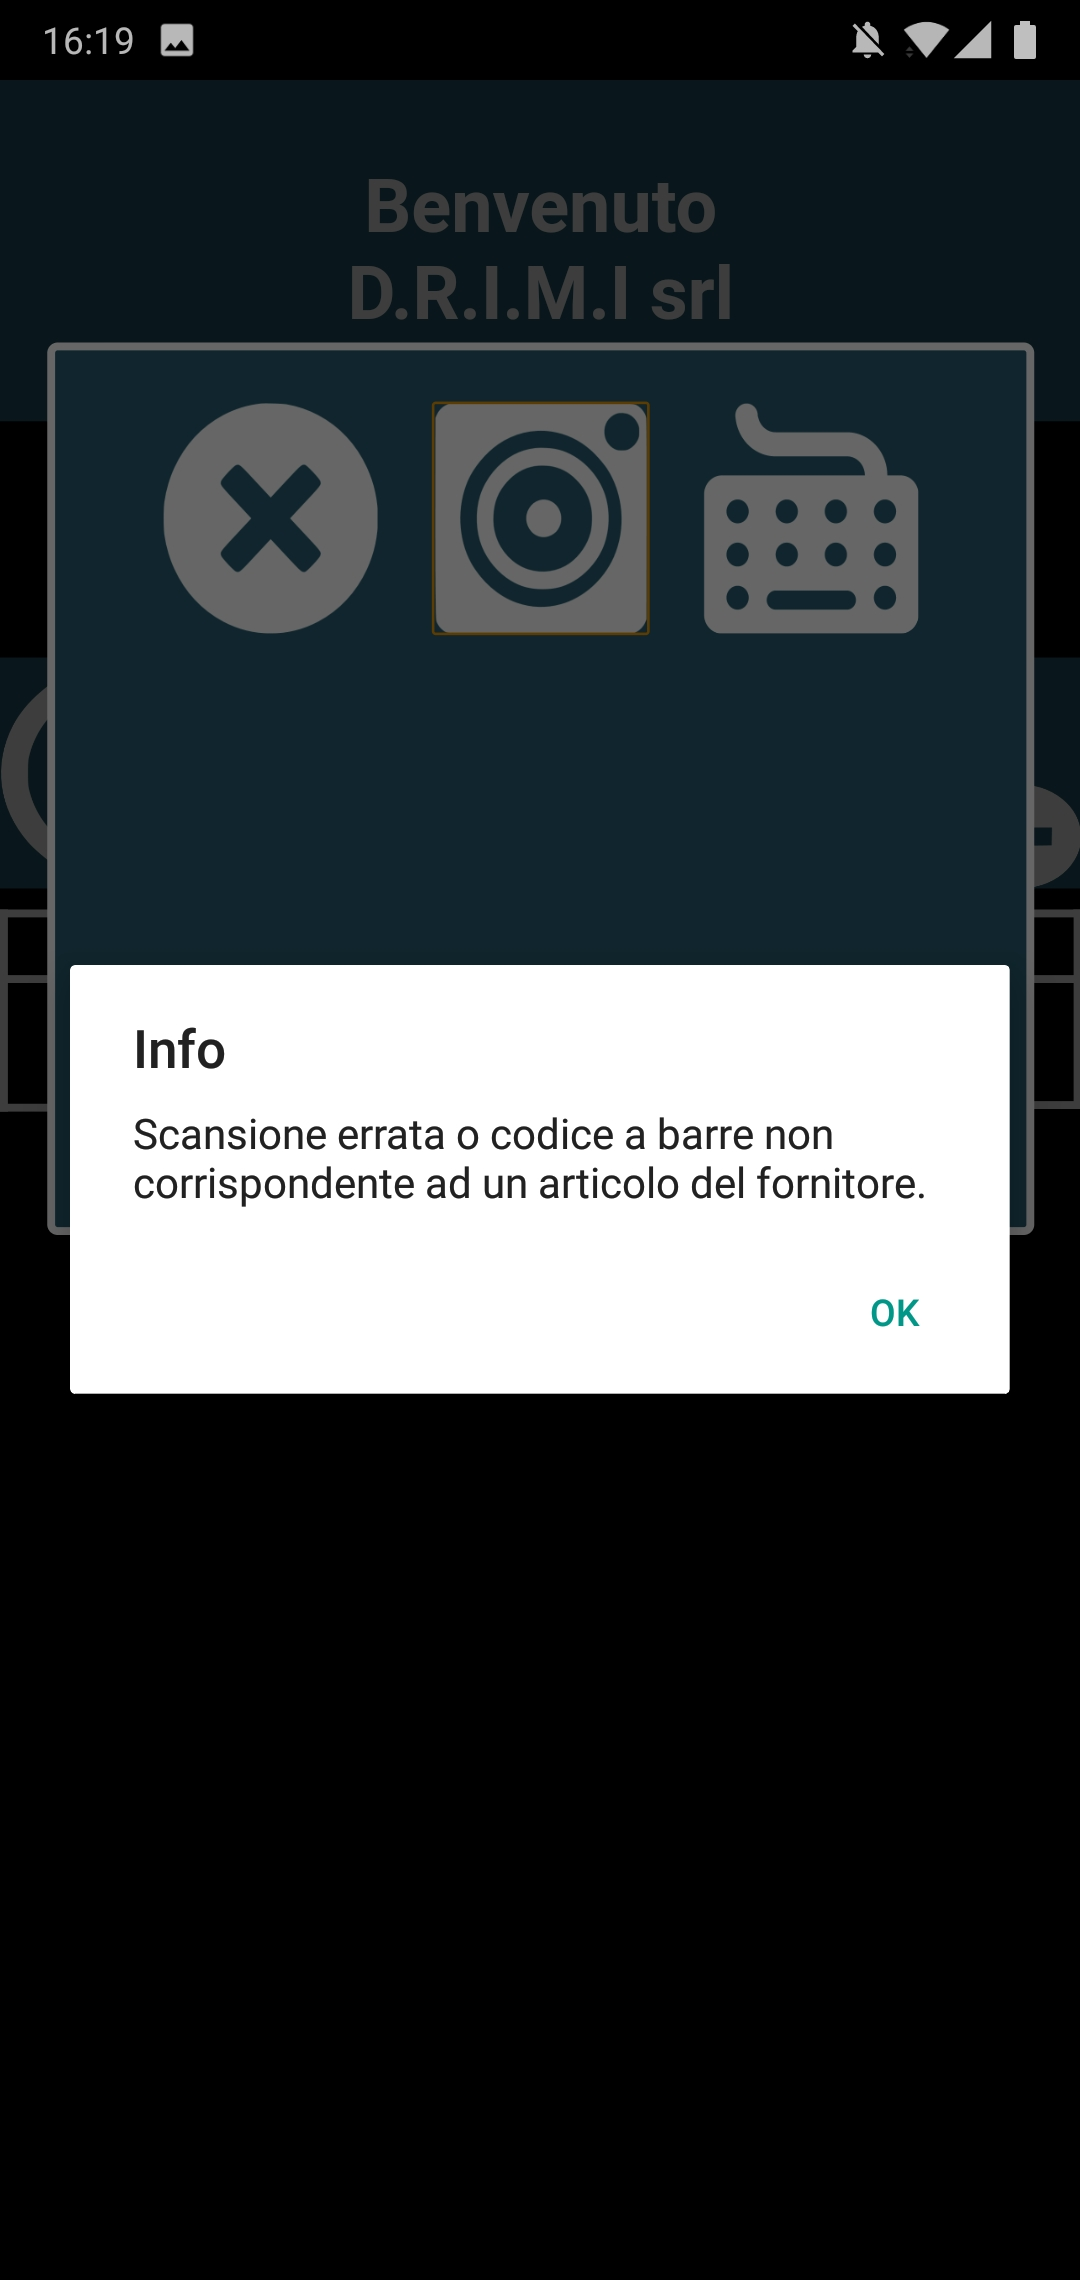
\includegraphics[width=.3\textwidth]{./img/erroreCodiceNonPresente.jpg}

\caption{Possibili casi durante la procedura di scansione di un codice a barre}

\end{figure}

\newpage

Tutti i casi possibili durante la digitazione del codice di un articolo sono i seguenti:
\begin{enumerate}
	\item Codice articolo inserito \textbf{correttamente}: dopo aver inserito un codice articolo corretto e aver premuto sul pulsante ``OK", verrà aperta
	la pagina per l'inserimento del nuovo articolo. La pagina viene aperta
	solamente se l'articolo non è già presente in carrello. In tal caso viene visualizzato un messaggio informativo che invita l'utente
	a modificarne la quantità direttamente dal carrello;
	\item Codice articolo \textbf{non inserito}: se viene premuto il pulsante ``OK" senza aver digitato un codice, viene visualizzato un messaggio
	informativo che invita l'utente ad inserire un codice;
	\item Codice articolo \textbf{non corrispondente ad un articolo venduto} dal fornitore: in questo caso l'utente può aver inserito il codice in
	maniera non corretta, oppure si tratta del codice di un articolo che non corrisponde a quello di un articolo venduto dal fornitore. In 
	questo caso viene visualizzato un messaggio d'errore per notificare all'utente l'errore nella digitazione del codice articolo.
\end{enumerate}

\begin{figure}[h]

\centering
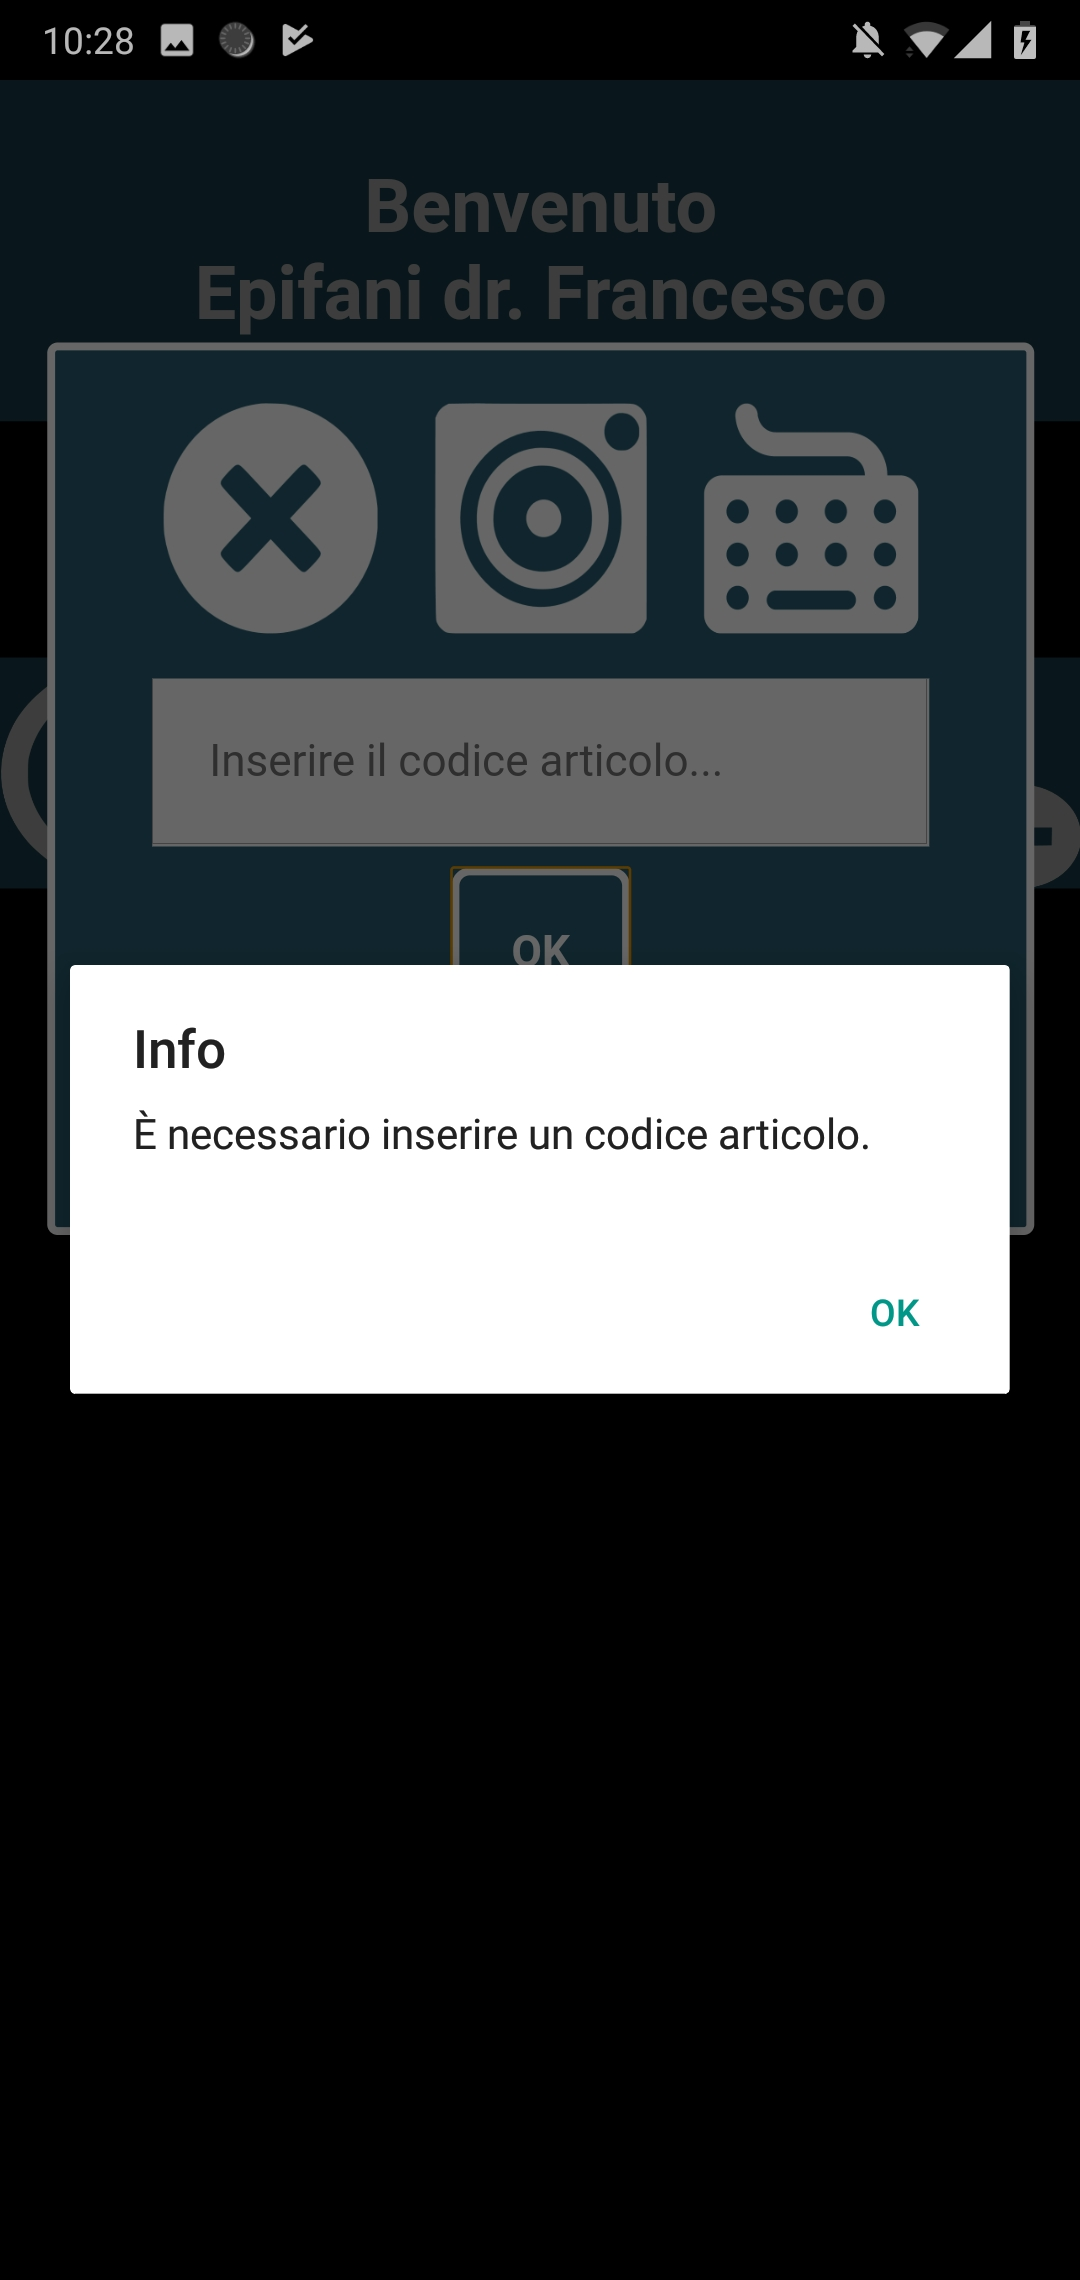
\includegraphics[width=.3\textwidth]{./img/erroreNonInserito.jpg}\hfill
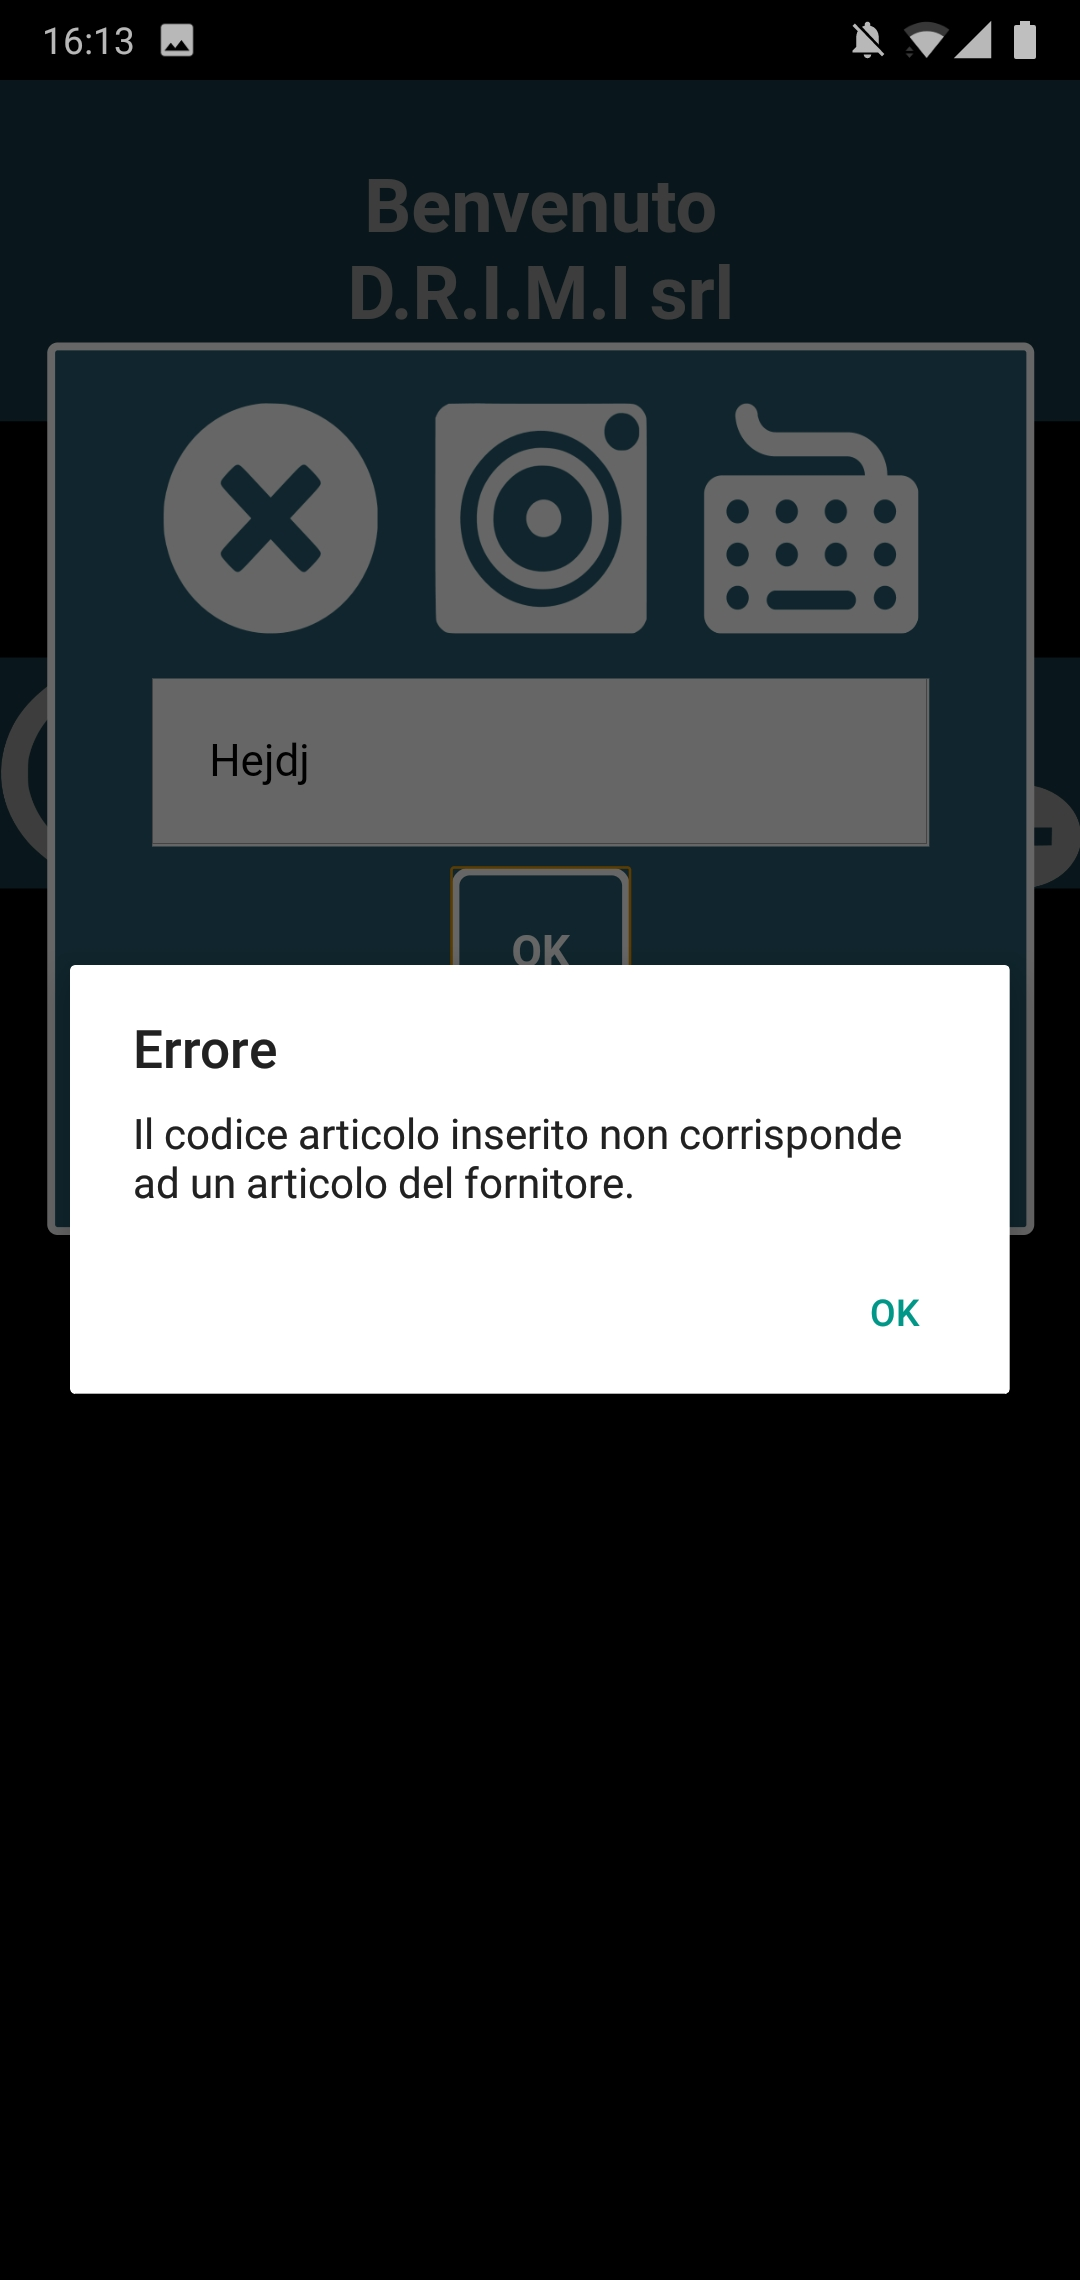
\includegraphics[width=.3\textwidth]{./img/erroreArticolo.jpg}\hfill
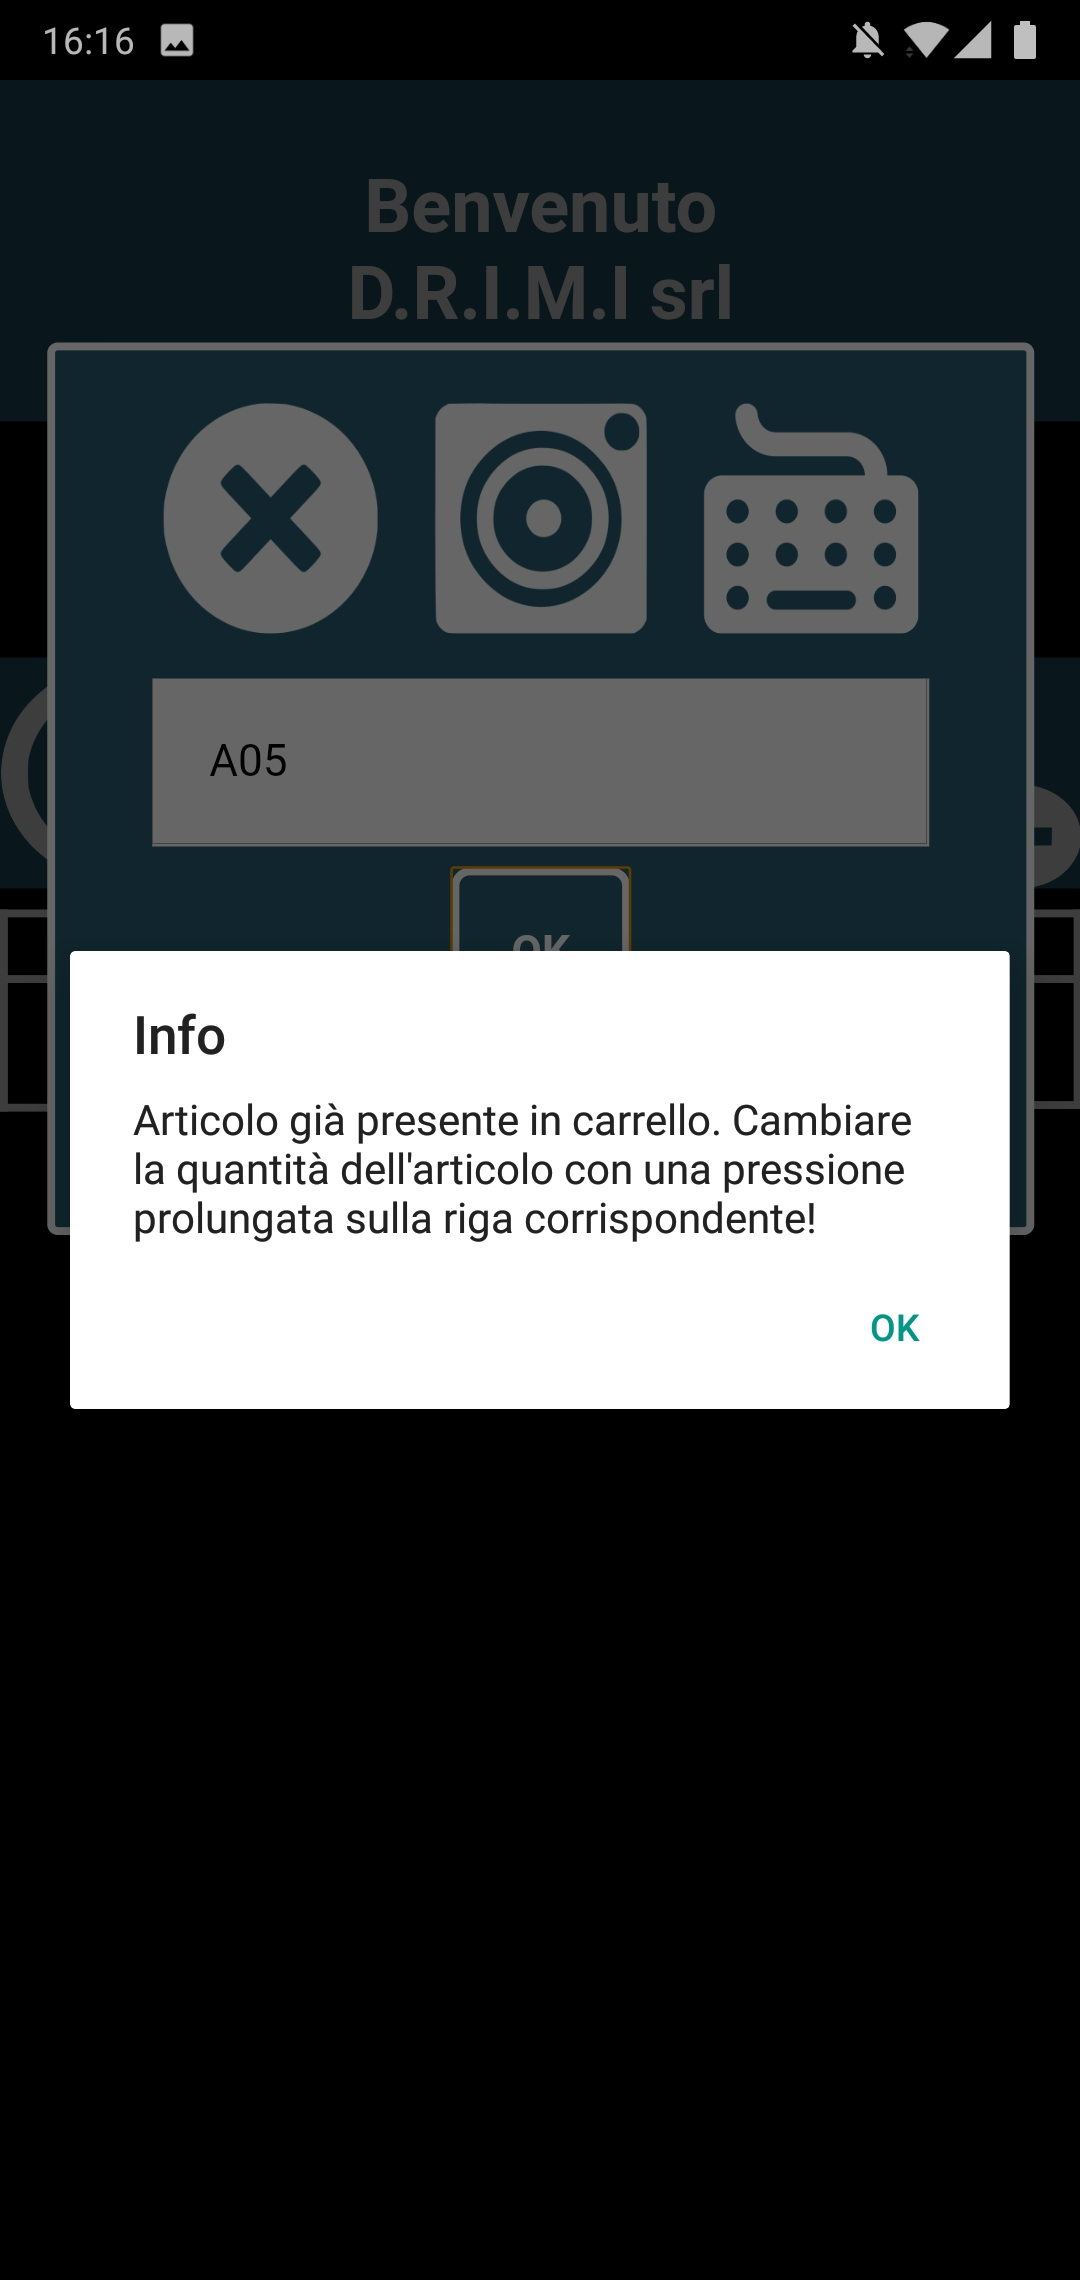
\includegraphics[width=.3\textwidth]{./img/erroreArticoloPresente.jpg}

\caption{Possibili casi durante la procedura di digitazione del codice di un articolo}

\end{figure}

Infine, se sul modal per l'inserimento di un nuovo articolo viene premuto il pulsante ``X", verrà chiuso il modal per l'inserimento di
un nuovo articolo e si tornerà al carrello.

\newpage

\myparagraph{Eliminazione di un articolo} \label{remove}

La procedura di eliminazione di un articolo consiste nel:
\begin{enumerate}
	\item Selezionare uno o più articoli dal carrello;
	\item Premere il pulsante di eliminazione degli articoli selezionati;
	\item Dare la conferma di eliminazione nel dialog box di conferma che verrà aperto dopo aver premuto il pulsante.
\end{enumerate}

Se tutti questi passi vengono eseguiti correttamente, e nell'ordine corretto, allora l'eliminazione andrà a buon fine, altrimenti nessuna modifica verrà effettuata al carrello.

Alcuni casi speciali potrebbero essere:
\begin{enumerate}
	\item Il pulsante viene premuto senza aver selezionato alcun articolo: viene visualizzato un messaggio che informa l'utente di dover
	selezionare almeno un articolo per dare inizio alla procedura di eliminazione;
	\item Il pulsante viene premuto senza nessun articolo in carrello: viene visualizzato il medesimo messaggio del punto precedente;
	\item Nel dialog box che richiede conferma per la cancellazione degli articoli selezionati viene premuto il pulsante ``Annulla": il
	carrello rimane inalterato senza aver rimosso alcun articolo.
\end{enumerate}

\begin{figure}[h]
	\centering
	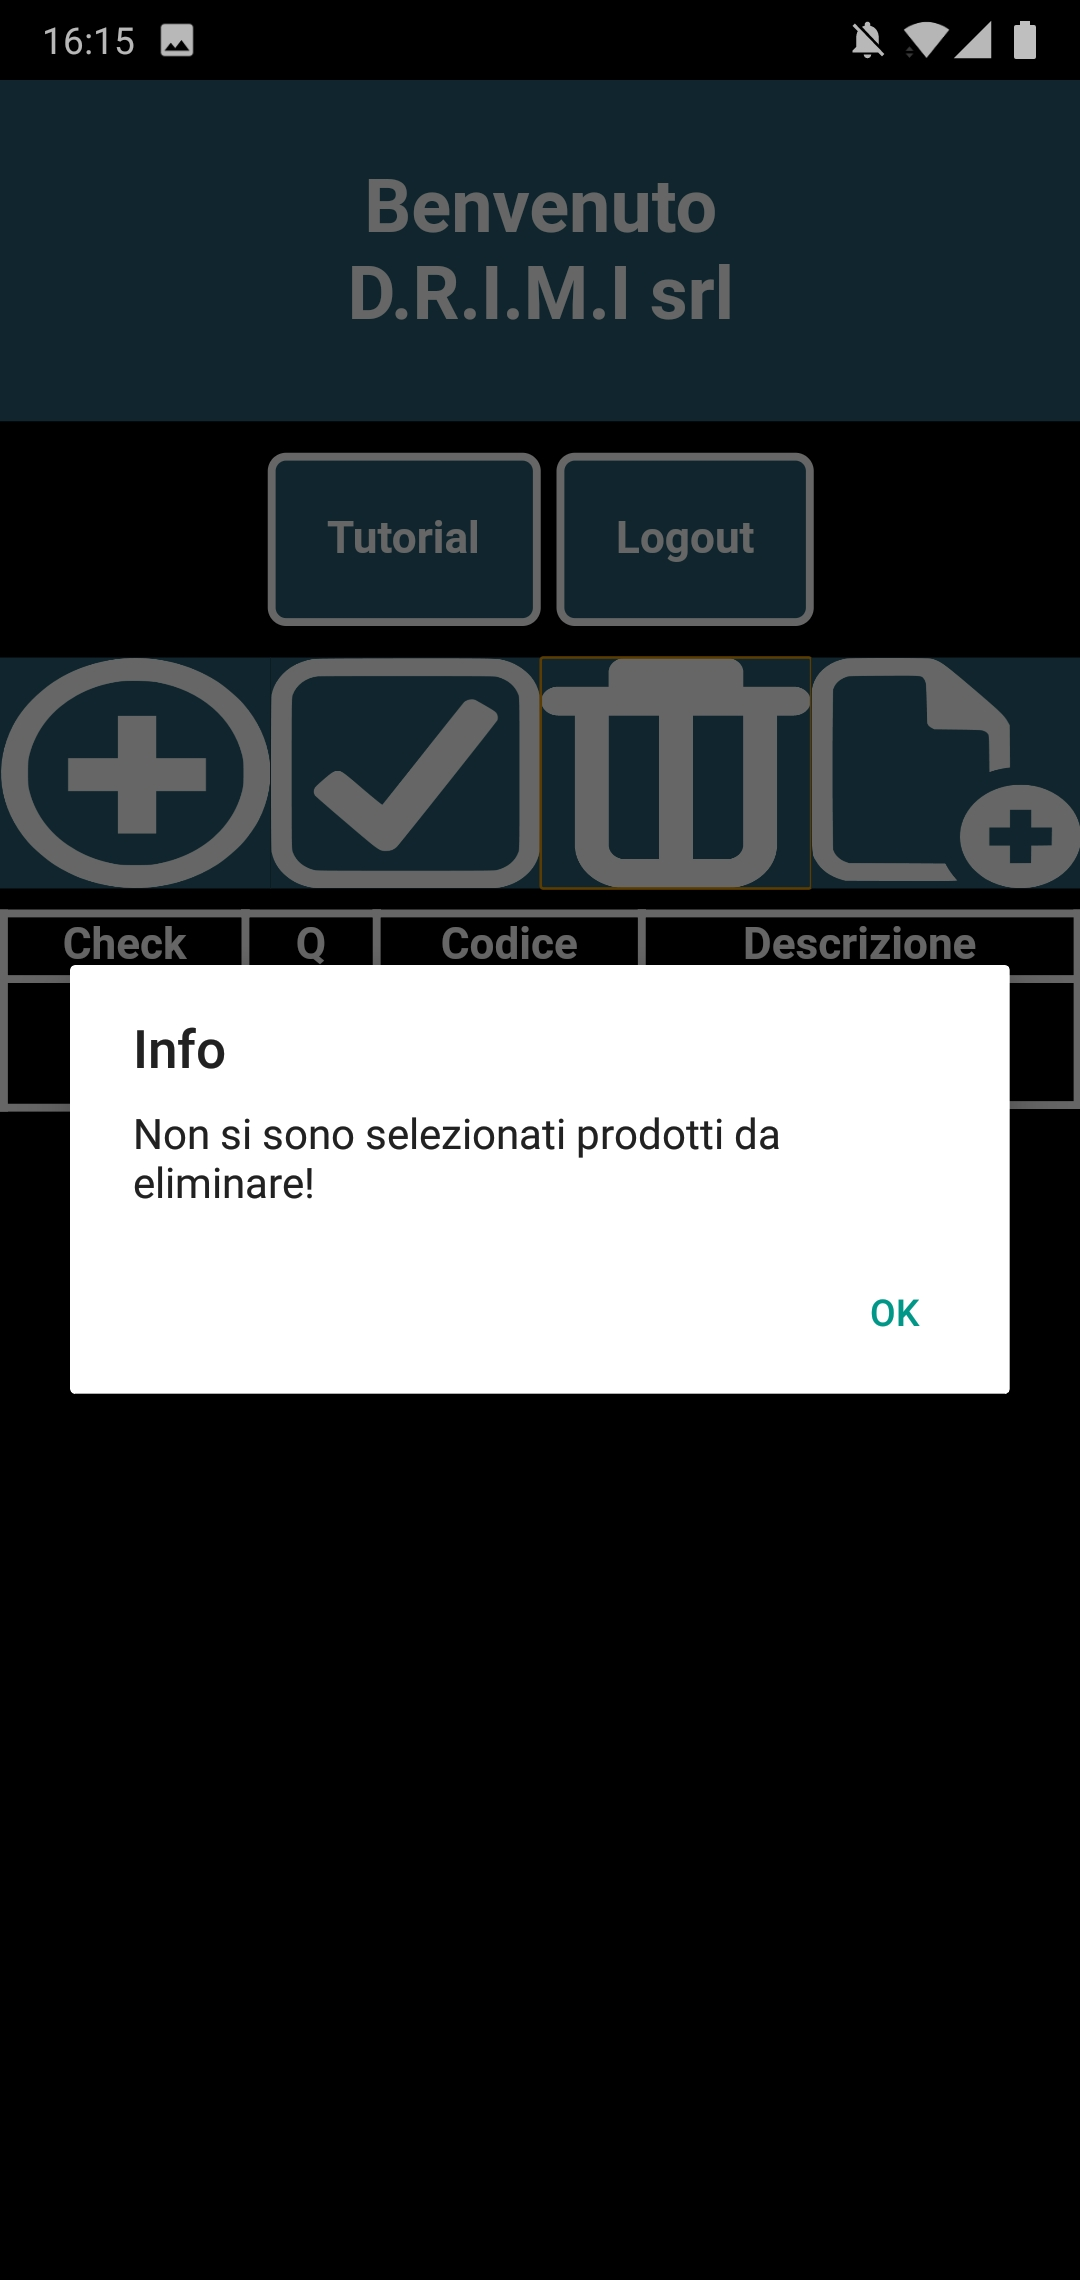
\includegraphics[width=.3\textwidth]{./img/erroreElim.jpg}
	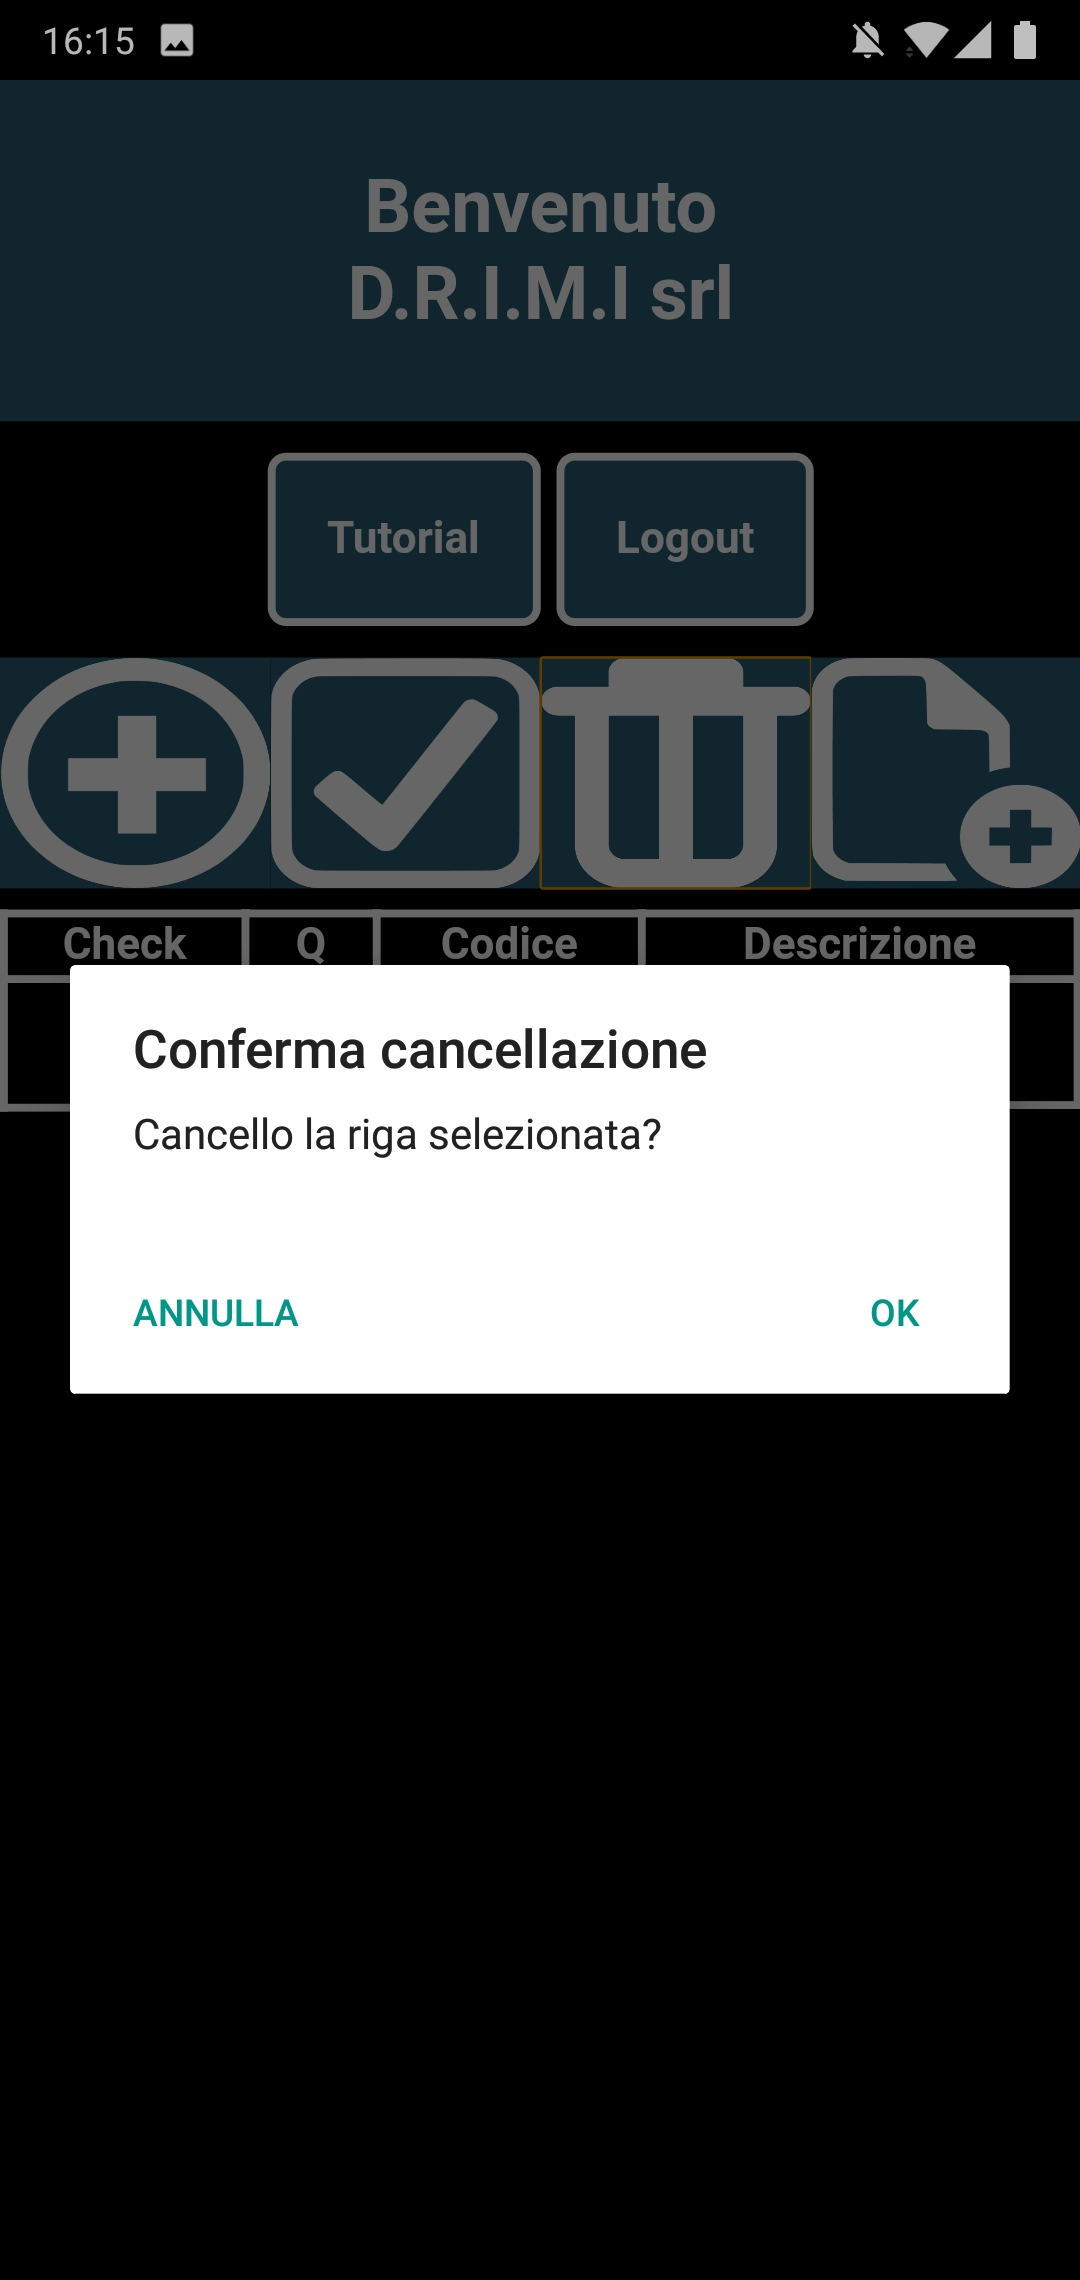
\includegraphics[width=.3\textwidth]{./img/confermaCanc.jpg}
	\caption[Possibili dialog sulla cancellazione di un articolo]{A sinistra il caso di articoli non selezionati per l'eliminazione; a destra il messaggio di conferma di cancellazione}
\end{figure}

 \newpage

\myparagraph{Modifica di un articolo}

La procedura di modifica di un articolo consiste nel:
\begin{enumerate}
	\item Premere sulla riga del carrello dell'articolo che si vuole modificare;
	\item Dare conferma di voler modificare l'articolo premendo ``OK" sul messaggio di conferma che apparirà dopo aver premuto sull'articolo;
	\item Procedere con la modifica dei dati d'ordine dell'articolo sulla pagina che verrà aperta dopo aver dato conferma di voler modificare
	l'articolo.
\end{enumerate}

\begin{figure}[h]
	\centering
	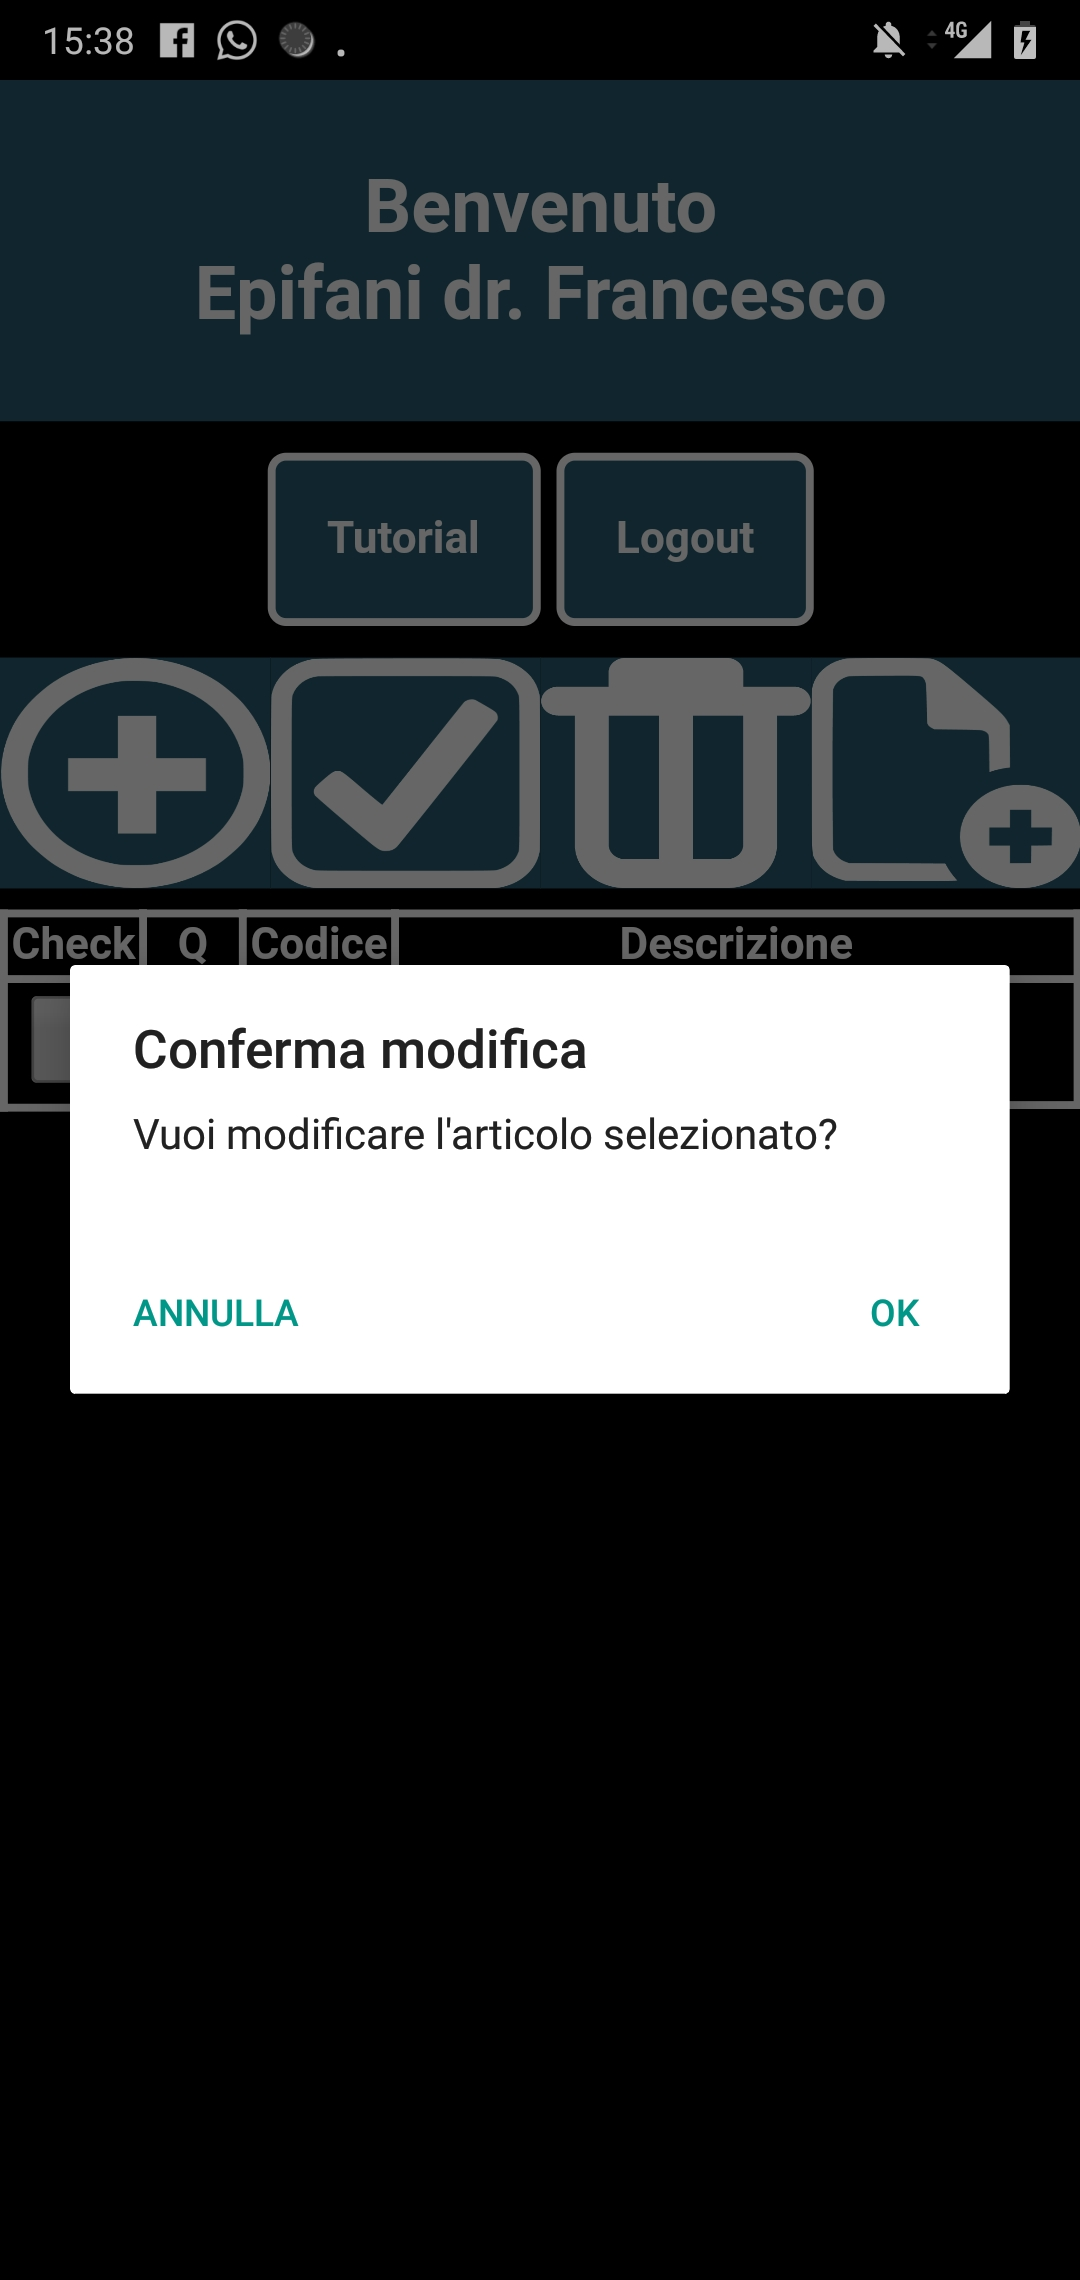
\includegraphics[width=.3\textwidth]{./img/confermaMod.jpg}
	\caption{Messaggio di richiesta di conferma di modifica}
\end{figure}

\newpage

\myparagraph{Creazione e invio di un ordine} \label{new}

\begin{figure}[h]
	\centering
	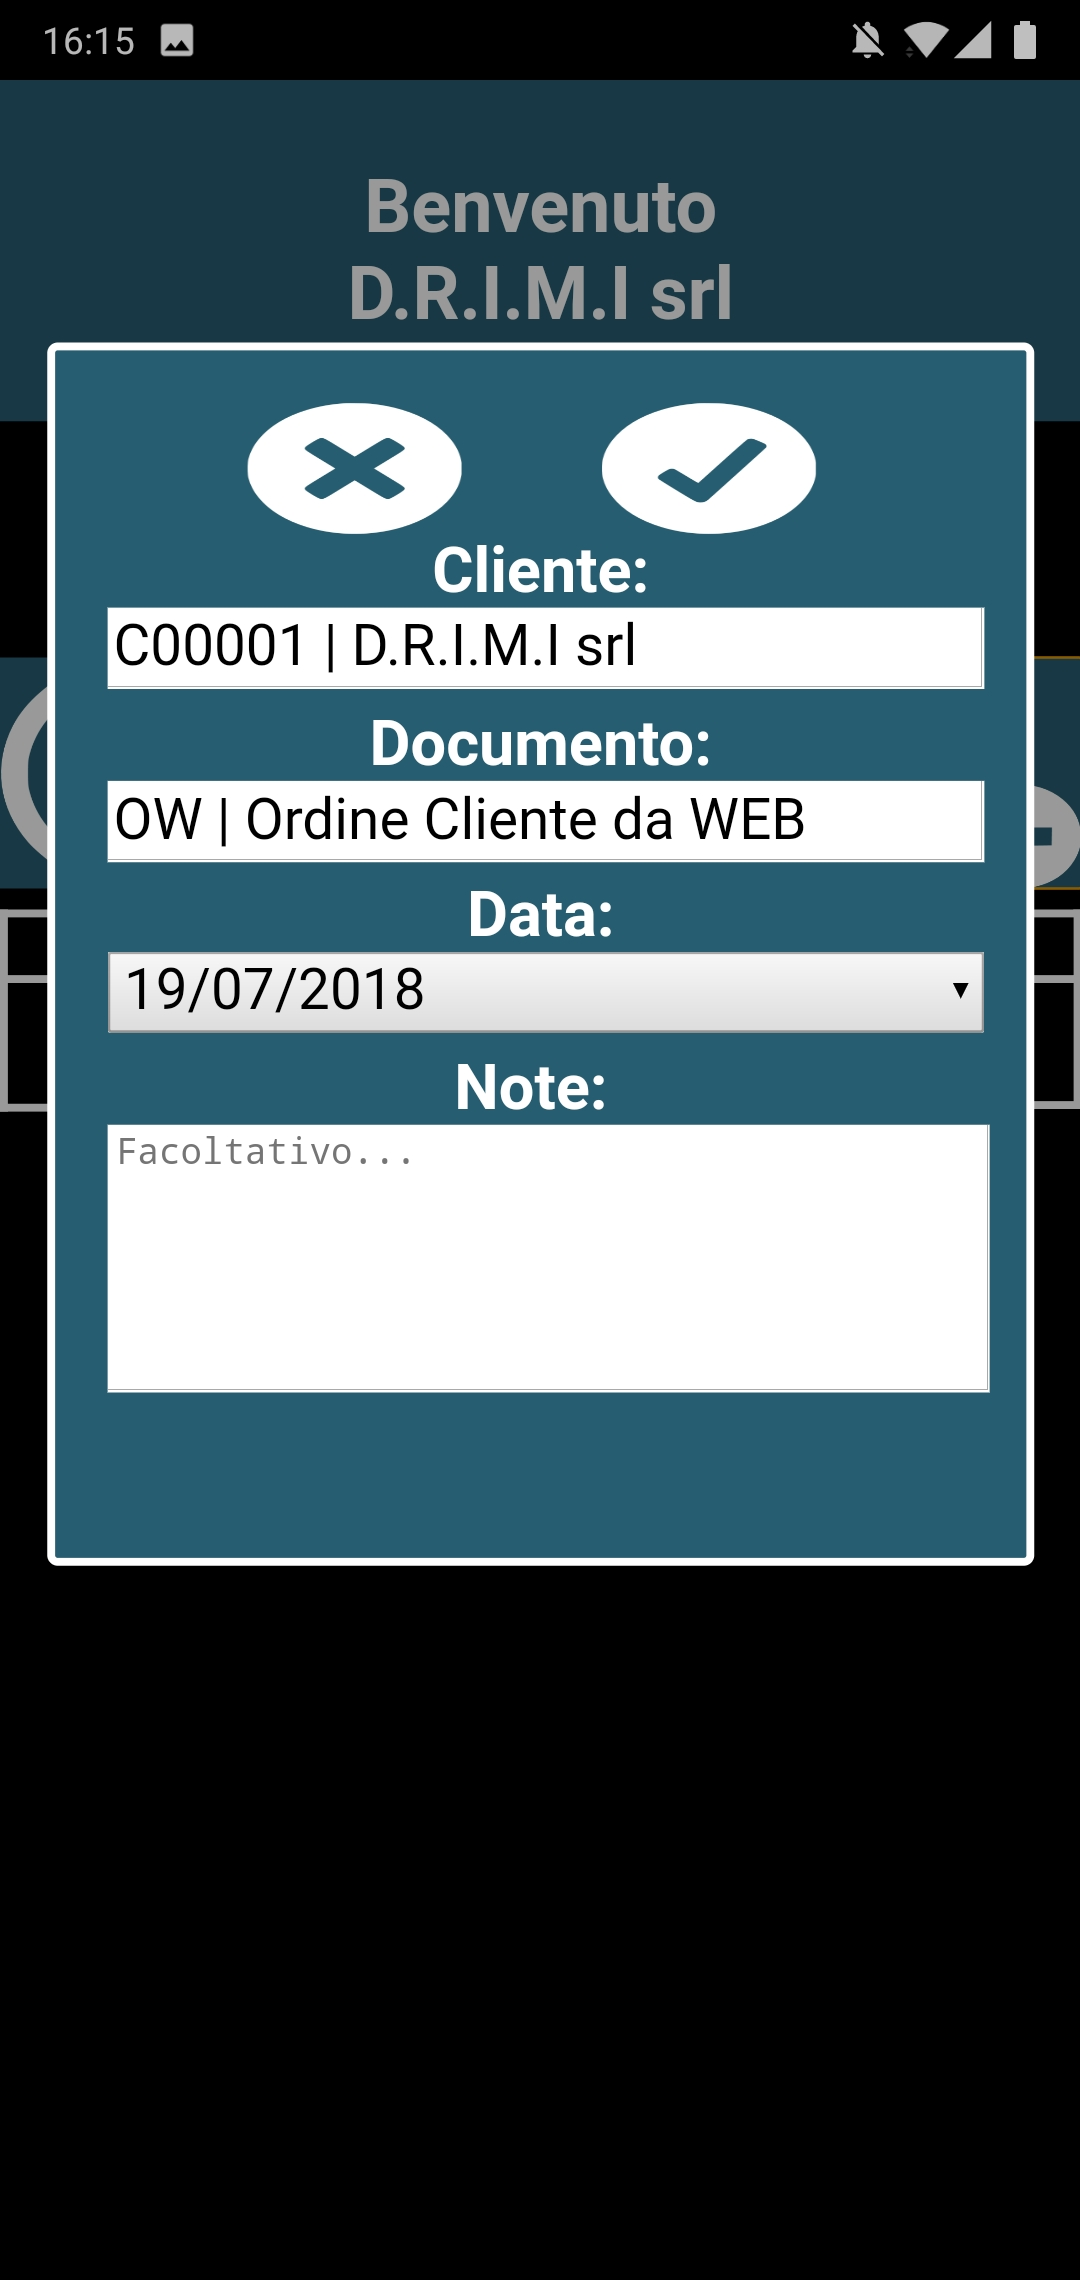
\includegraphics[width=.3\textwidth]{./img/modalFinale.jpg}
	\caption{Modal per la creazione e l'invio di un ordine}
\end{figure}

La procedura di creazione di un ordine consiste nel:
\begin{enumerate}
	\item Selezionare l'articolo o gli articoli che si vogliono ordinare premendo sulla check-box corrispondente;
	\item Premere sul pulsante ``crea ordine" (quarto pulsante della griglia dei pulsanti). Se il pulsante viene premuto senza aver selezionato alcun articolo, verrà visualizzato un messaggio informativo che invita l'utente a selezionare un articolo da ordinare;
	\item Compilare il form sul modal aperto in seguito alla pressione del pulsante;
	\item Premere sul pulsante ``V" per confermare e inviare l'ordine.
\end{enumerate} 

Dopo aver premuto sul pulsante ``crea ordine" viene aperto un modal che permette l'inserimento di alcuni dati utili alla creazione di un ordine. Il modal per la creazione di un ordine ha la seguente struttura, a partire dall'alto verso il basso:
\begin{itemize}
	\item \textbf{Testata}: nella testata del modal sono presenti due pulsanti:
		\begin{enumerate}
			\item ``\textbf{V}": pulsante di conferma e invio dell'ordine. Alla pressione del pulsante, viene richiesta la conferma per l'invio dell'ordine e, se la risposta è affermativa, l'ordine viene inviato e viene notificato all'utente che gli verrà inviata una mail di conferma.
			Dopo aver chiuso il messaggio di notifica, viene chiuso il modal e visualizzato il carrello. Il carrello non conterrà più gli articoli appena ordinati;
			\item ``\textbf{X}": pulsante di annullamento dell'ordine. Alla pressione del pulsante, il modal viene chiuso e viene visualizzato il carrello su cui non sarà stata apportata alcuna modifica.
		\end{enumerate}
	\item \textbf{Riga cliente}: è una input box in sola lettura che contiene il codice e il nome del cliente;
	\item \textbf{Riga documento}: è una input box in sola lettura che contiene il codice e il nome del documento che verrà generato per il cliente;
	\item \textbf{Data}: è una select box dove può essere inserita la data dell'ordine. Viene proposta la data odierna. Premendo sulla select verrà aperto il calendario per permettere l'inserimento veloce di una data;
	\item \textbf{Note}: è una text area dove possono essere inserite delle note per l'ordine. Le note sono facoltative.
\end{itemize}

\begin{figure}[h]

\centering
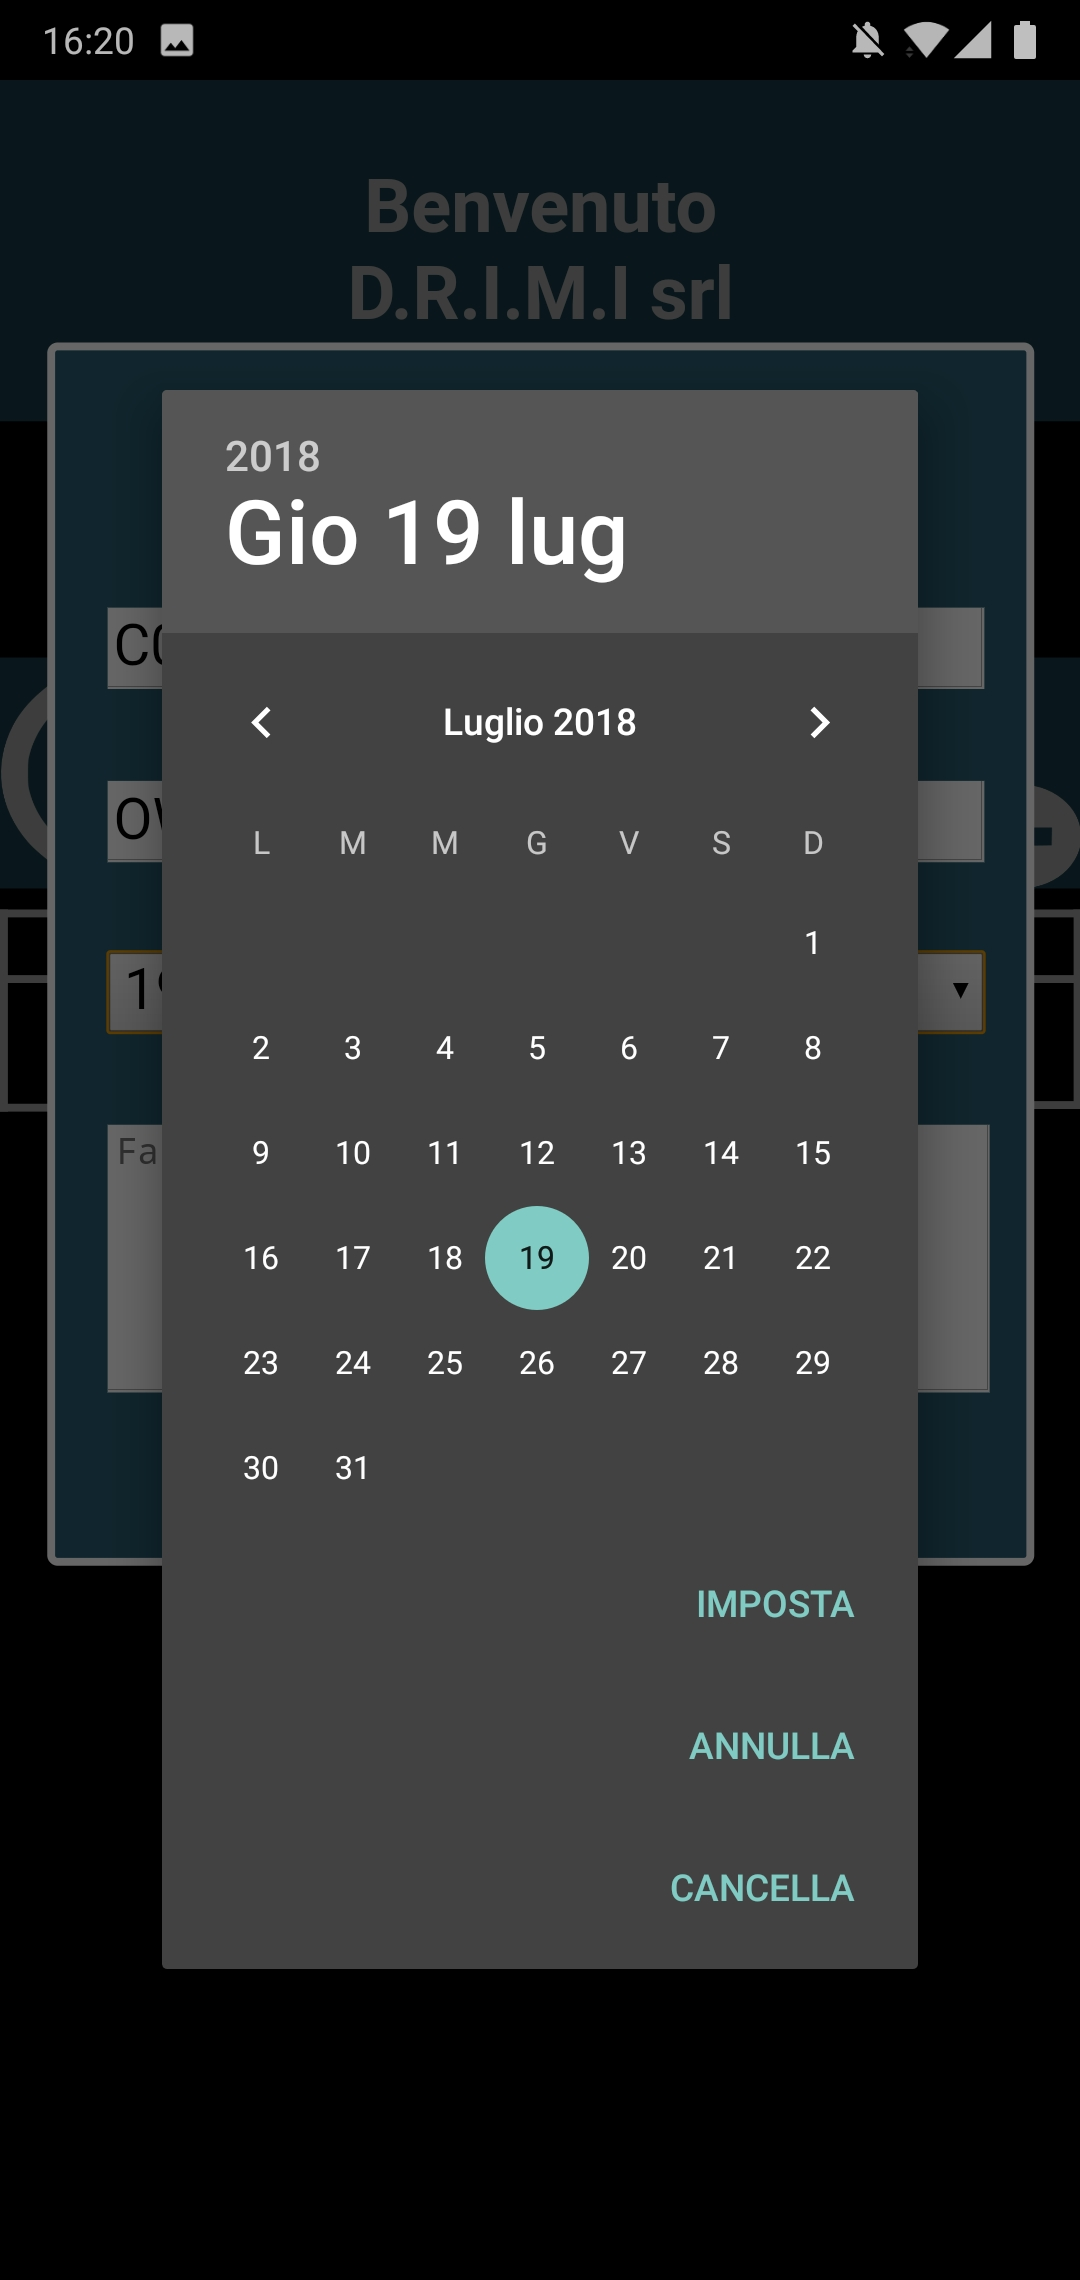
\includegraphics[width=.3\textwidth]{./img/data.jpg}\hfill
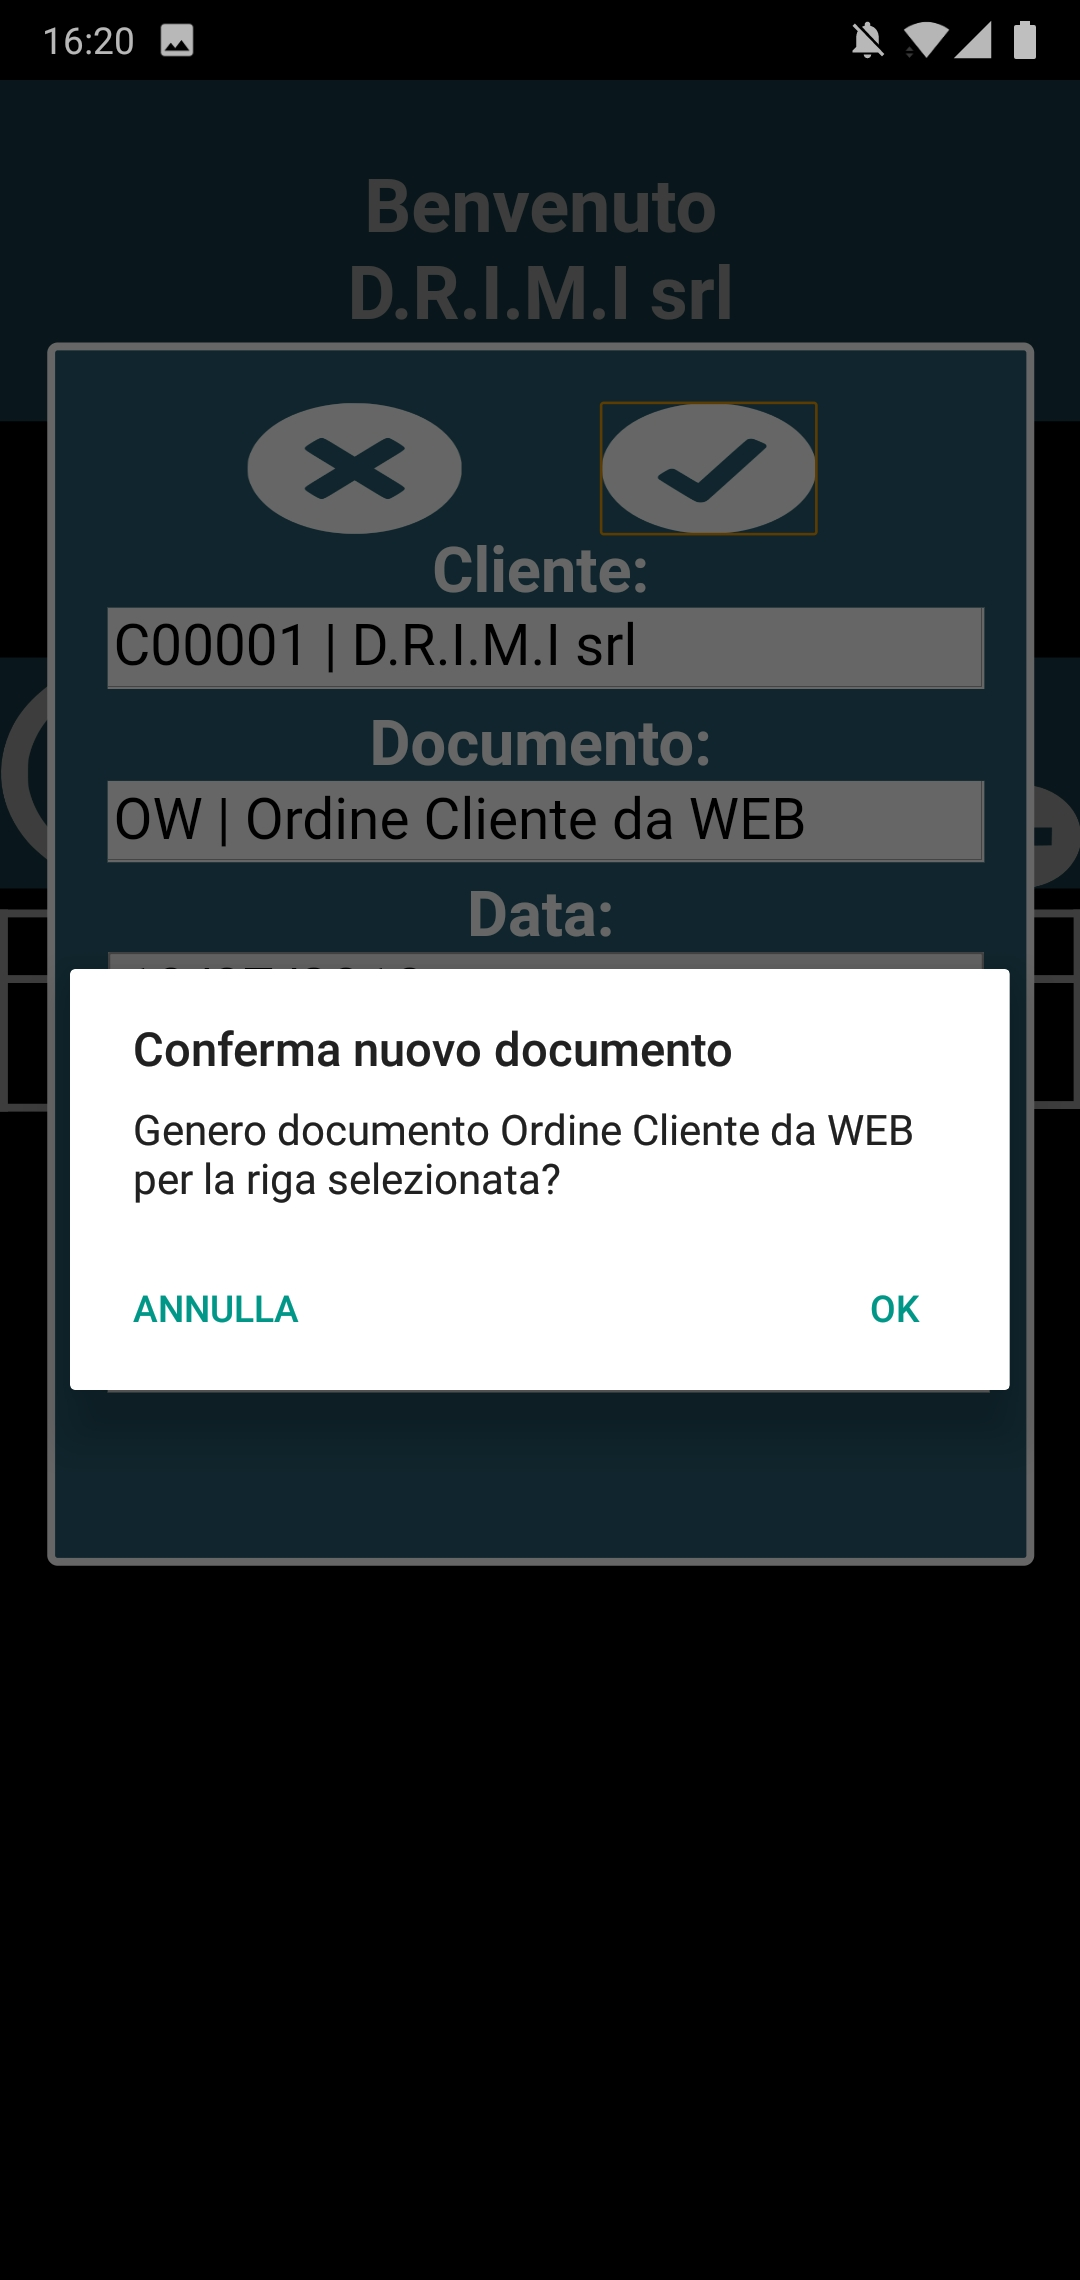
\includegraphics[width=.3\textwidth]{./img/confermaDoc.jpg}\hfill
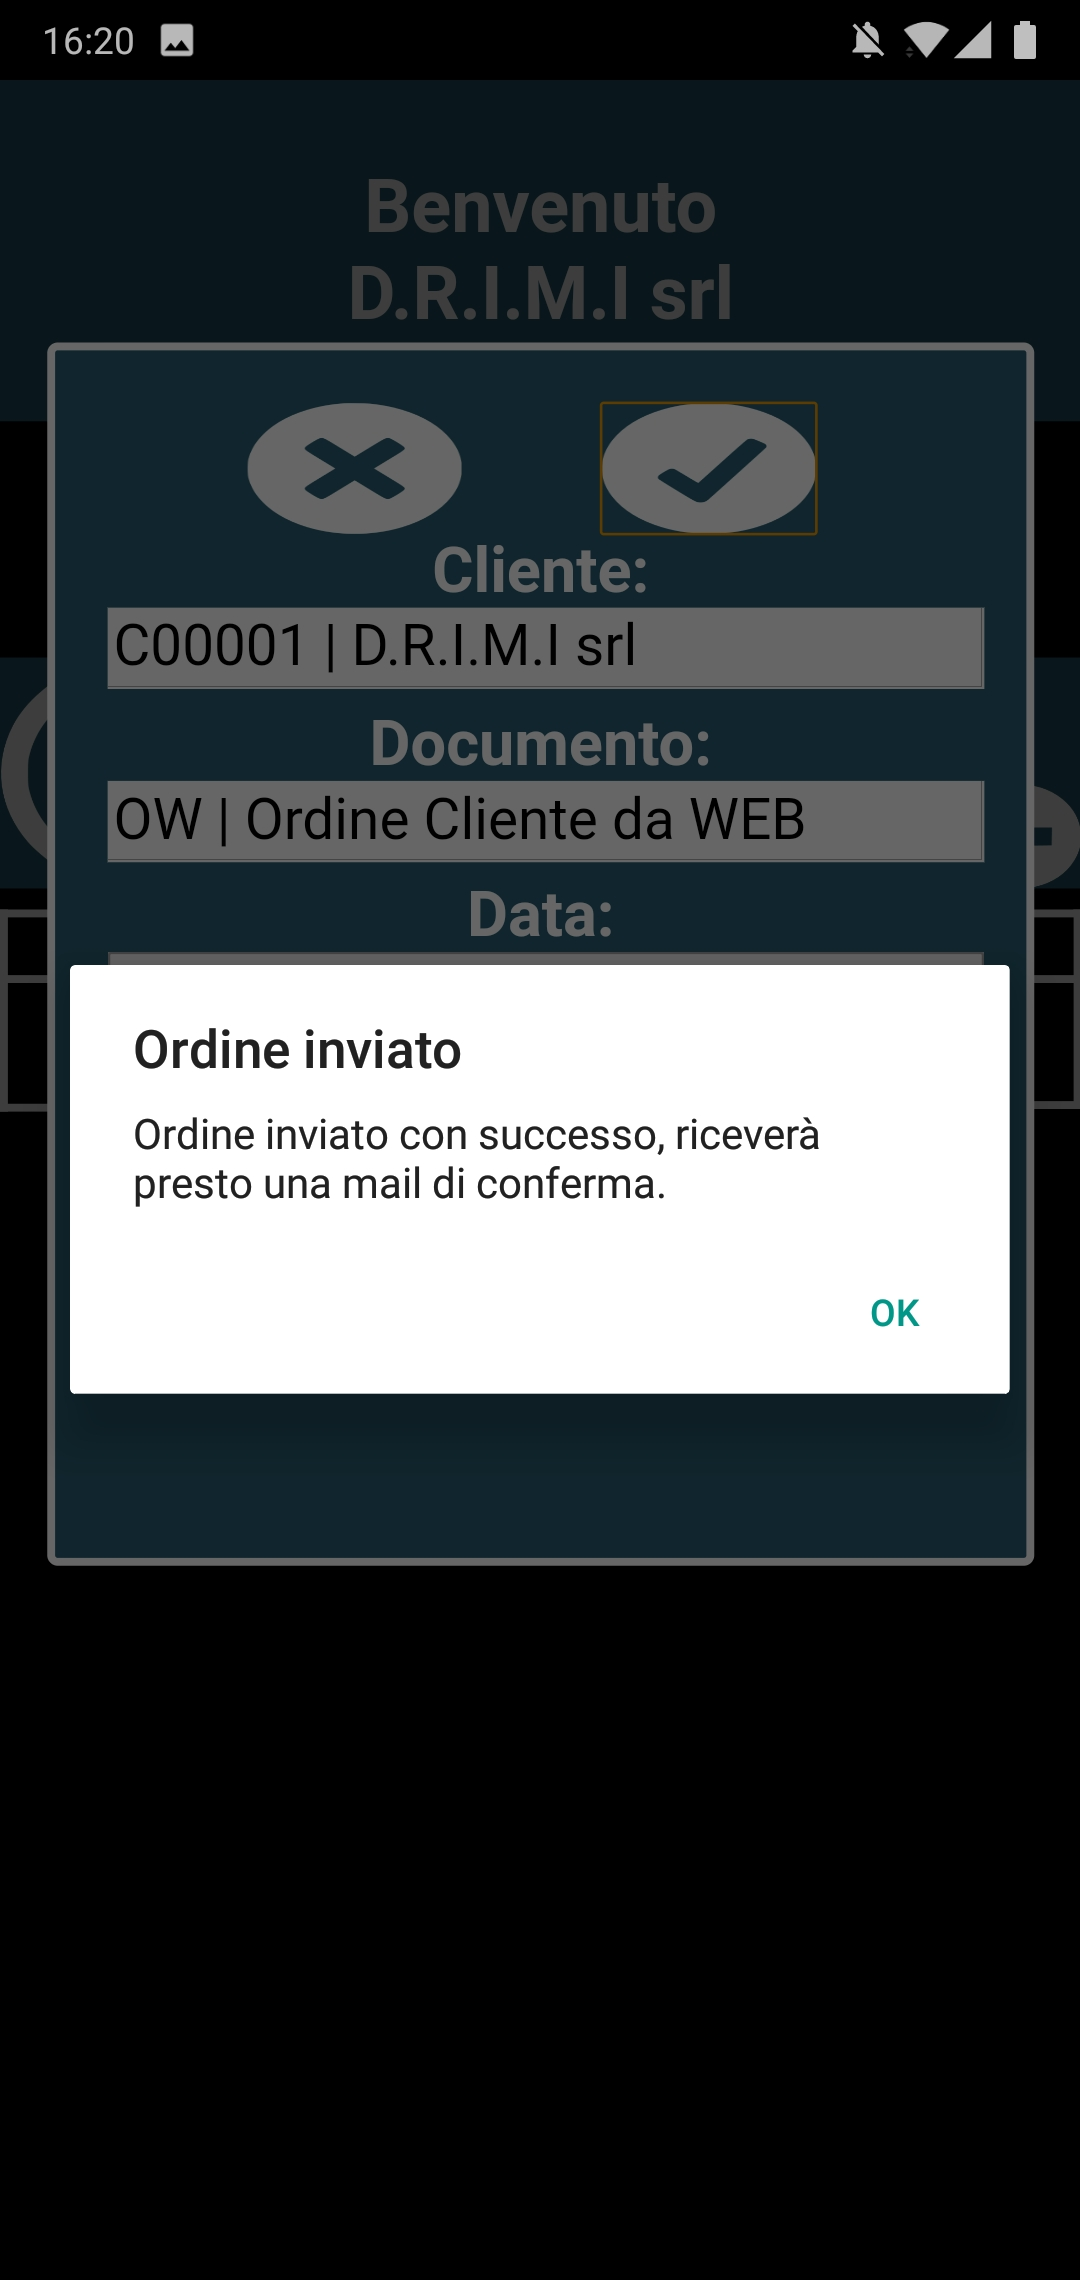
\includegraphics[width=.3\textwidth]{./img/confermaOrd.jpg}

\caption[Possibili finestre sul modal di invio di un ordine]{A sinistra il modal per l'inserimento di una data, al centro il messaggio di conferma di invio ordine, a destra il messaggio di conferma di invio dell'ordine}

\end{figure}


\newpage
 
 \subsection{Pagina di inserimento di un articolo}
 
\begin{figure}[h]
	\centering
	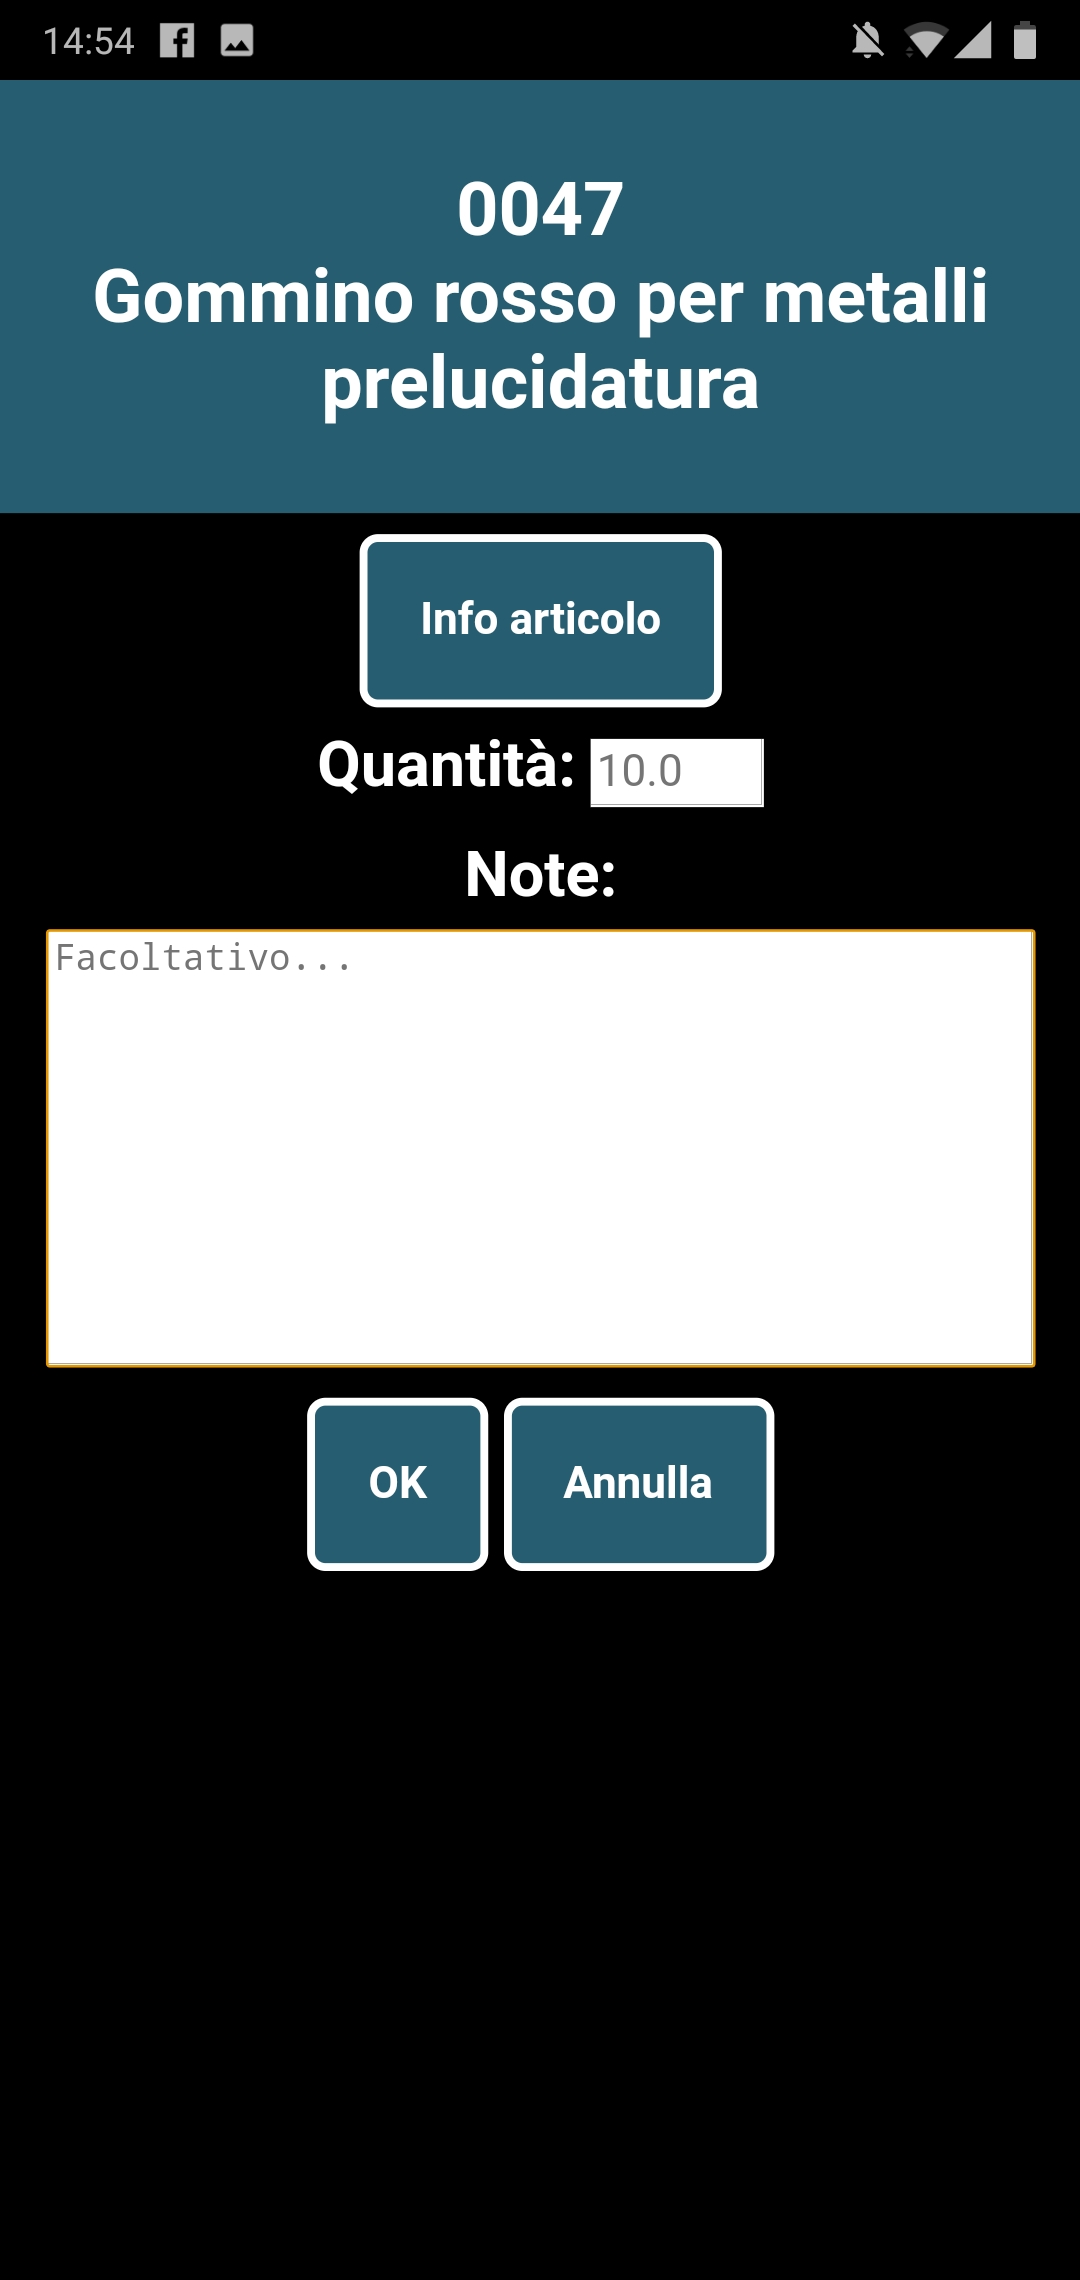
\includegraphics[width=.3\textwidth,height=9cm]{./img/notePresenti.jpg}
	\caption{Pagina di inserimento di un articolo}
\end{figure}
 
La pagina per l'inserimento di un articolo può essere aperta tramite il modal per l'inserimento di un nuovo articolo. Questa pagina è
costituita dalle seguenti quattro parti, a partire dall'altro verso il basso:
\begin{itemize}
	\item \textbf{Testata} della pagina: contiene il codice dell'articolo seguito dal nome dell'articolo;
	\item Pulsante ``\textbf{Info articolo}": se il pulsante viene premuto, un dialog box visualizzerà le note dell'articolo. È possibile che il bordo
	e il testo del pulsante siano rossi; in tal caso significa che non sono presenti delle note per l'articolo. Se il pulsante viene premuto
	comunque, verrà visualizzato un dialog box che notifichi che non esistono delle note per l'articolo;
	\item \textbf{Quantità}: è una input box dove l'utente può inserire la quantità dell'articolo che desidera ordinare. La quantità
	minima acquistabile è proposta all'apertura della pagina. Se l'utente dovesse inserire una quantità minore di quella proposta, o che non rispetti dei
	multipli richiesti, allora verrà visualizzato un dialog box che specifica la tipologia di errore commesso. Inoltre, la quantità è un campo obbligatorio, quindi se non dovesse essere inserita, verrà visualizzato un messaggio d'errore;
	\item \textbf{Note}: è una text area dove l'utente può inserire delle note sull'ordine per l'articolo che sta acquistando. Queste note sono
	facoltative.
\end{itemize}

Al termine della pagina sono presenti due pulsanti con le seguenti funzioni:
\begin{enumerate}
	\item \textbf{OK}: se il pulsante ``OK" viene premuto, l'articolo verrà inserito correttamente nel carrello solo se rispetta i vincoli imposti sulla quantità (quantità minima e multipla);
	\item \textbf{Annulla}: se il pulsante ``Annulla" viene premuto, l'applicazione tornerà la home page e non ci sarà alcuna variazione al carrello.
\end{enumerate}

\newpage

\begin{figure}[h]
	\centering
	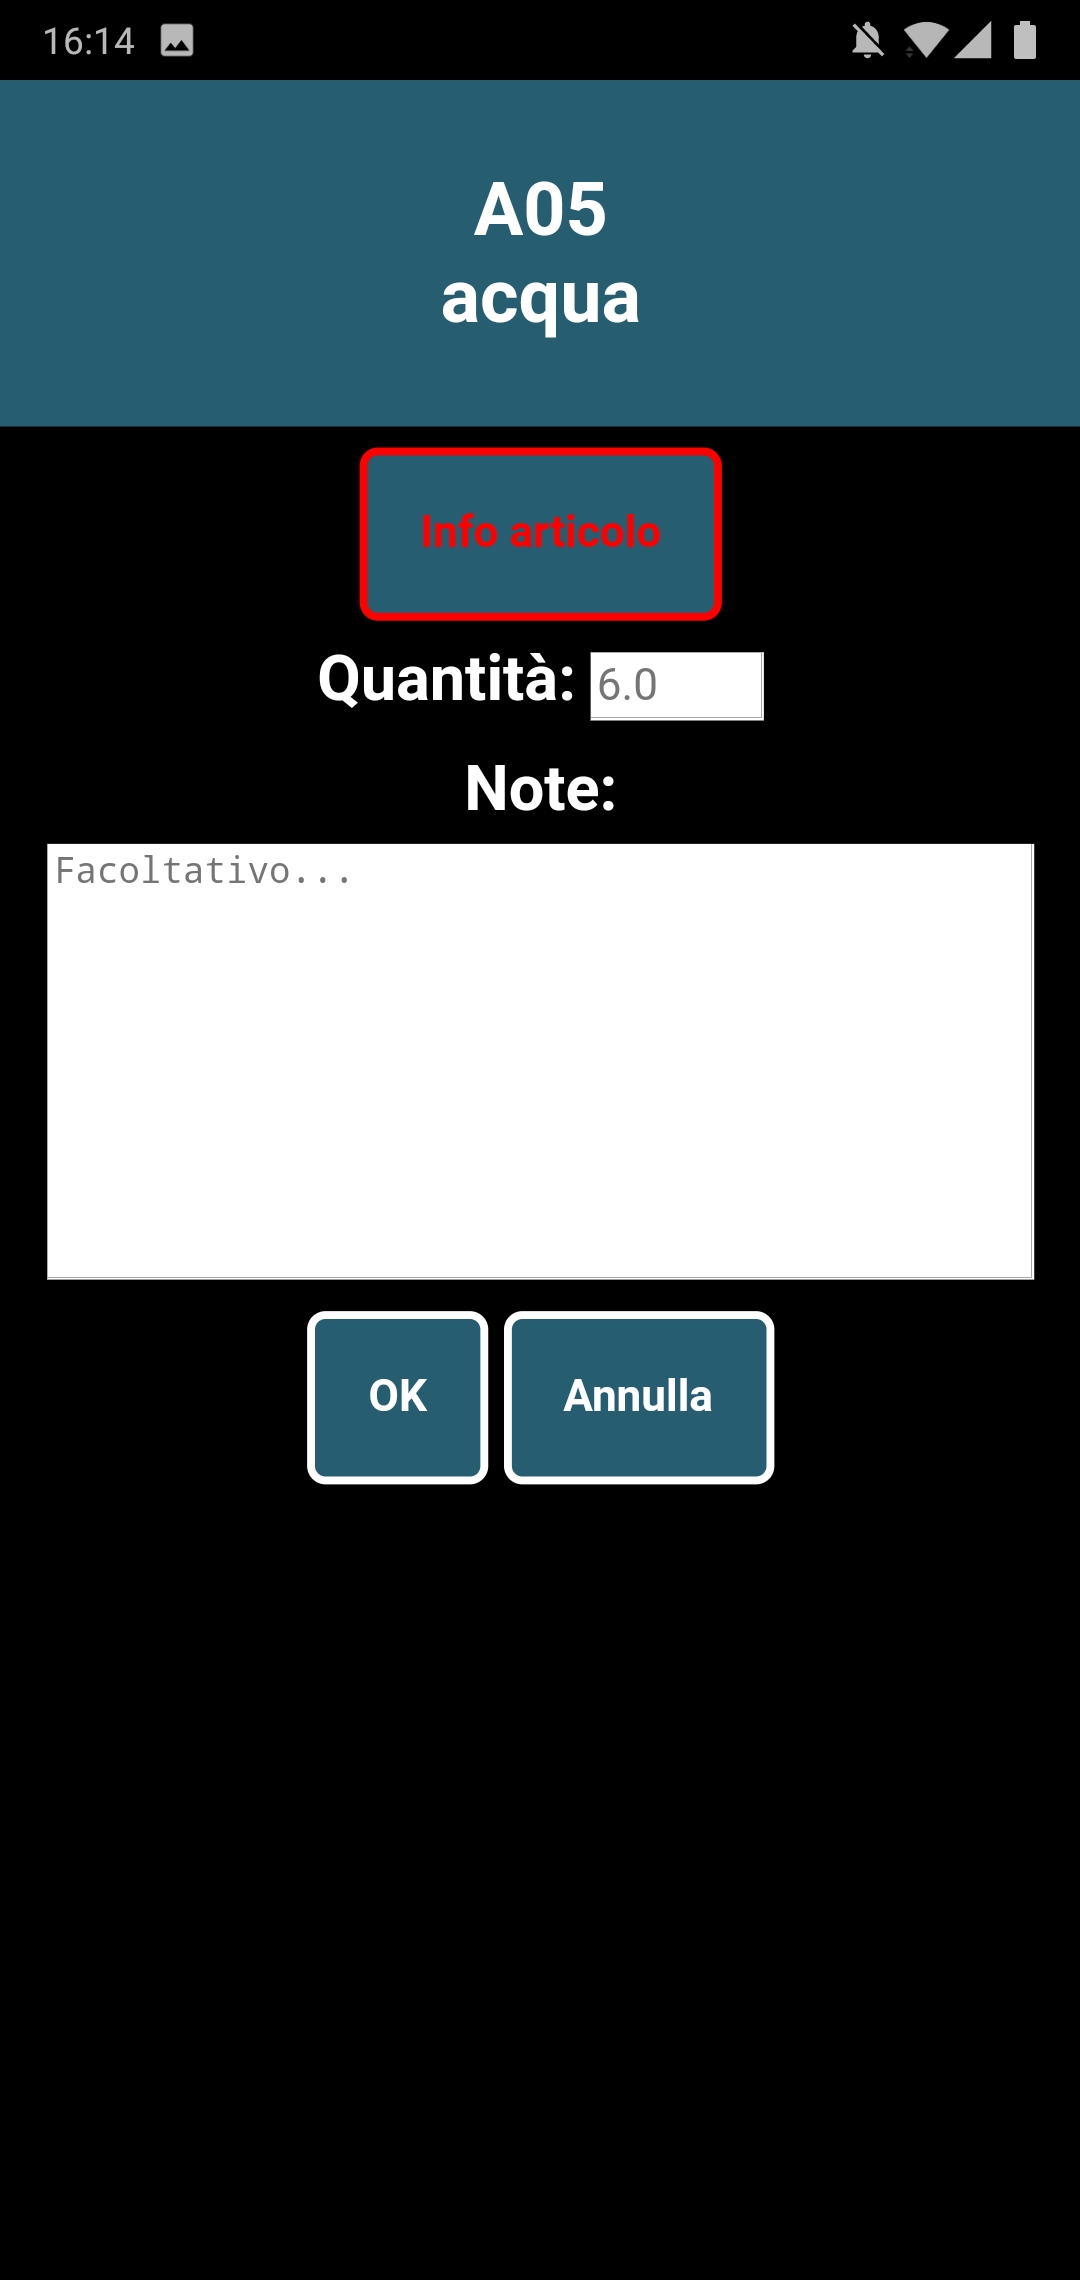
\includegraphics[width=.4\textwidth]{./img/paginaInsMod.jpg}
	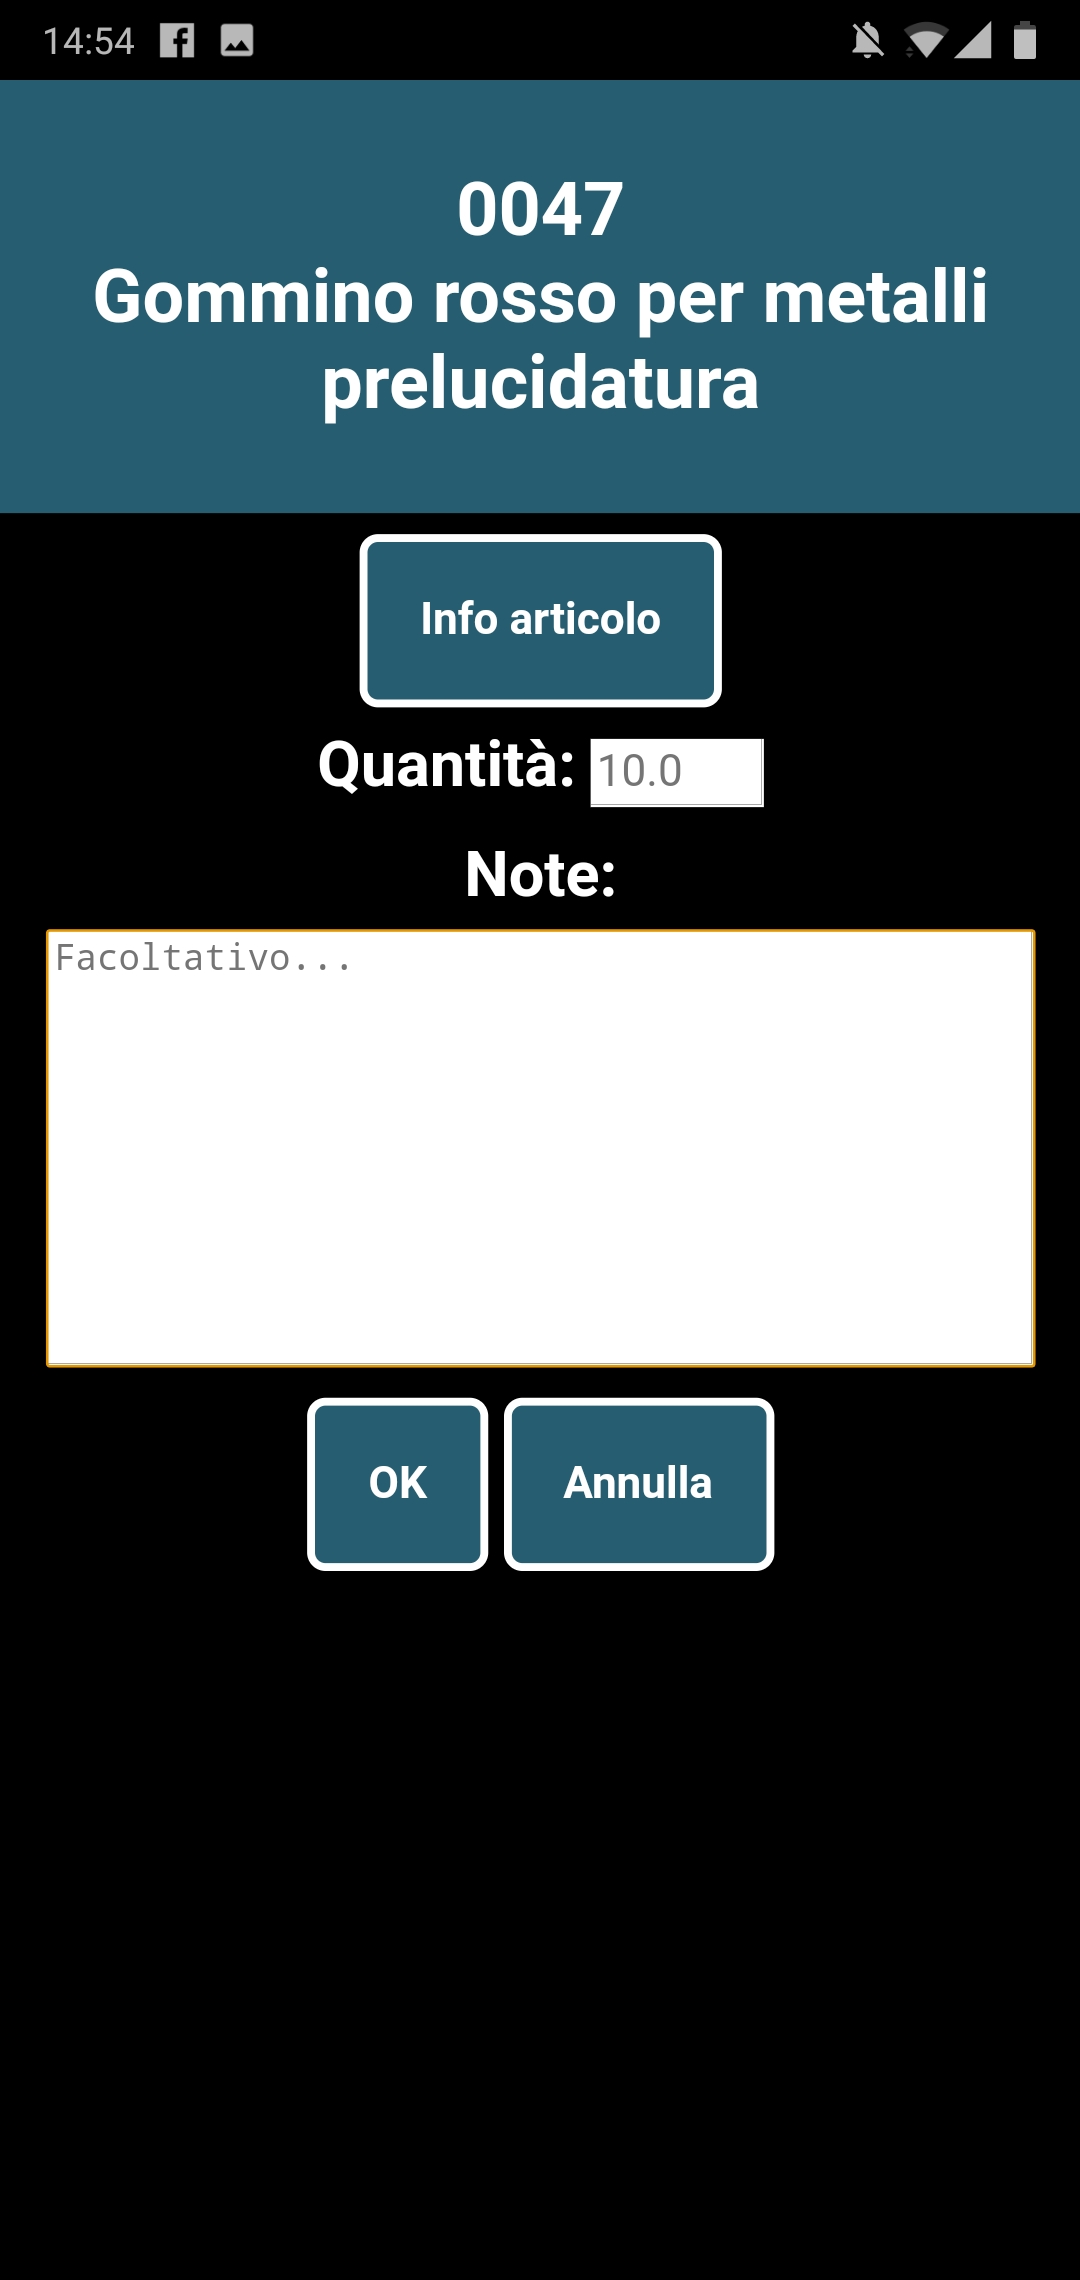
\includegraphics[width=.4\textwidth]{./img/notePresenti.jpg}
	\caption[Possibili casi sulla pagina di inserimento di un articolo]{A sinistra il caso di inserimento di un articolo senza note; a destra il caso di inserimento di un articolo con note}
\end{figure}

\newpage

\begin{figure}[h]
	\centering
	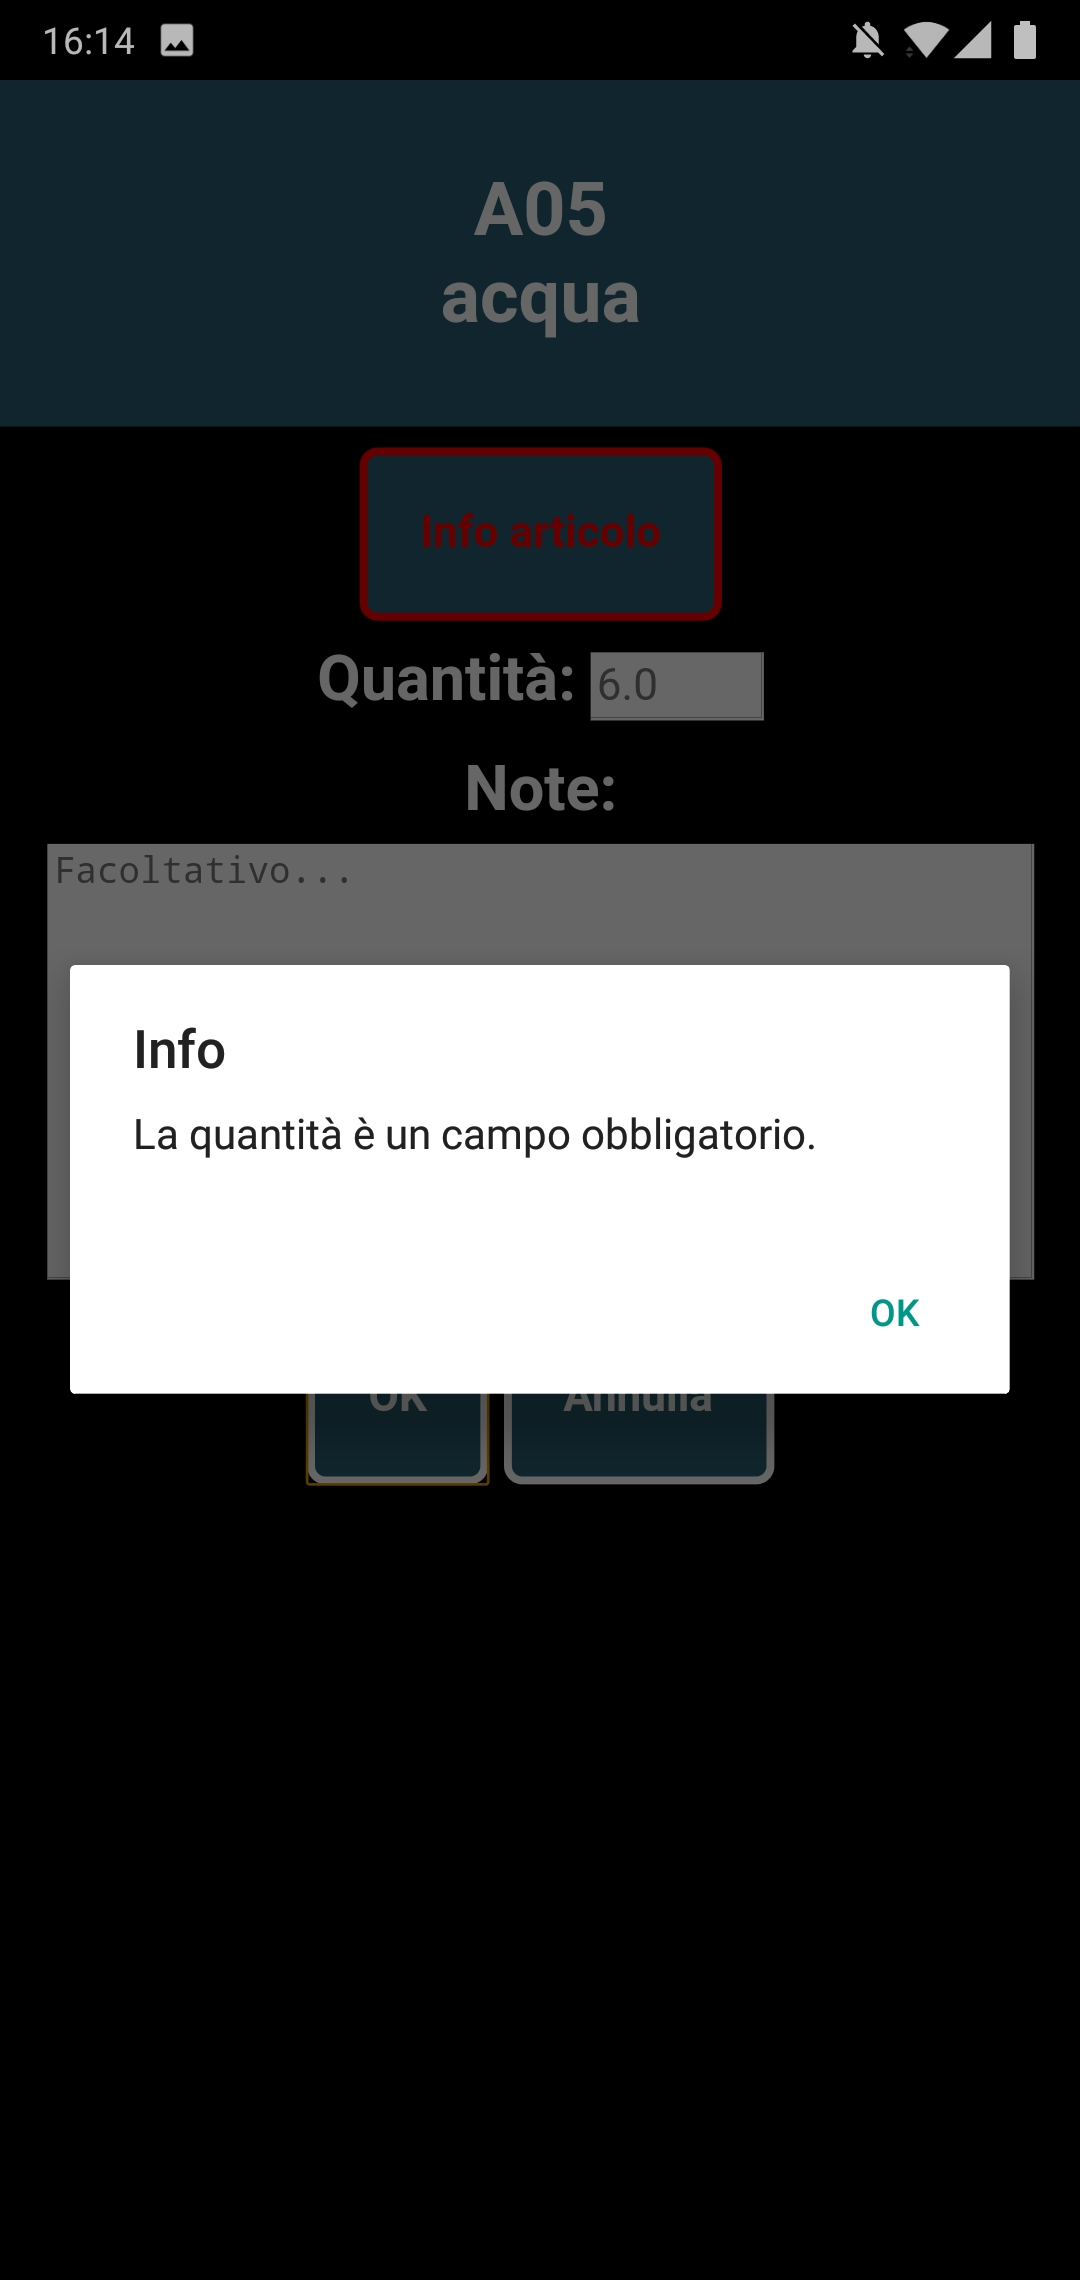
\includegraphics[width=.4\textwidth]{./img/erroreQta.jpg}
	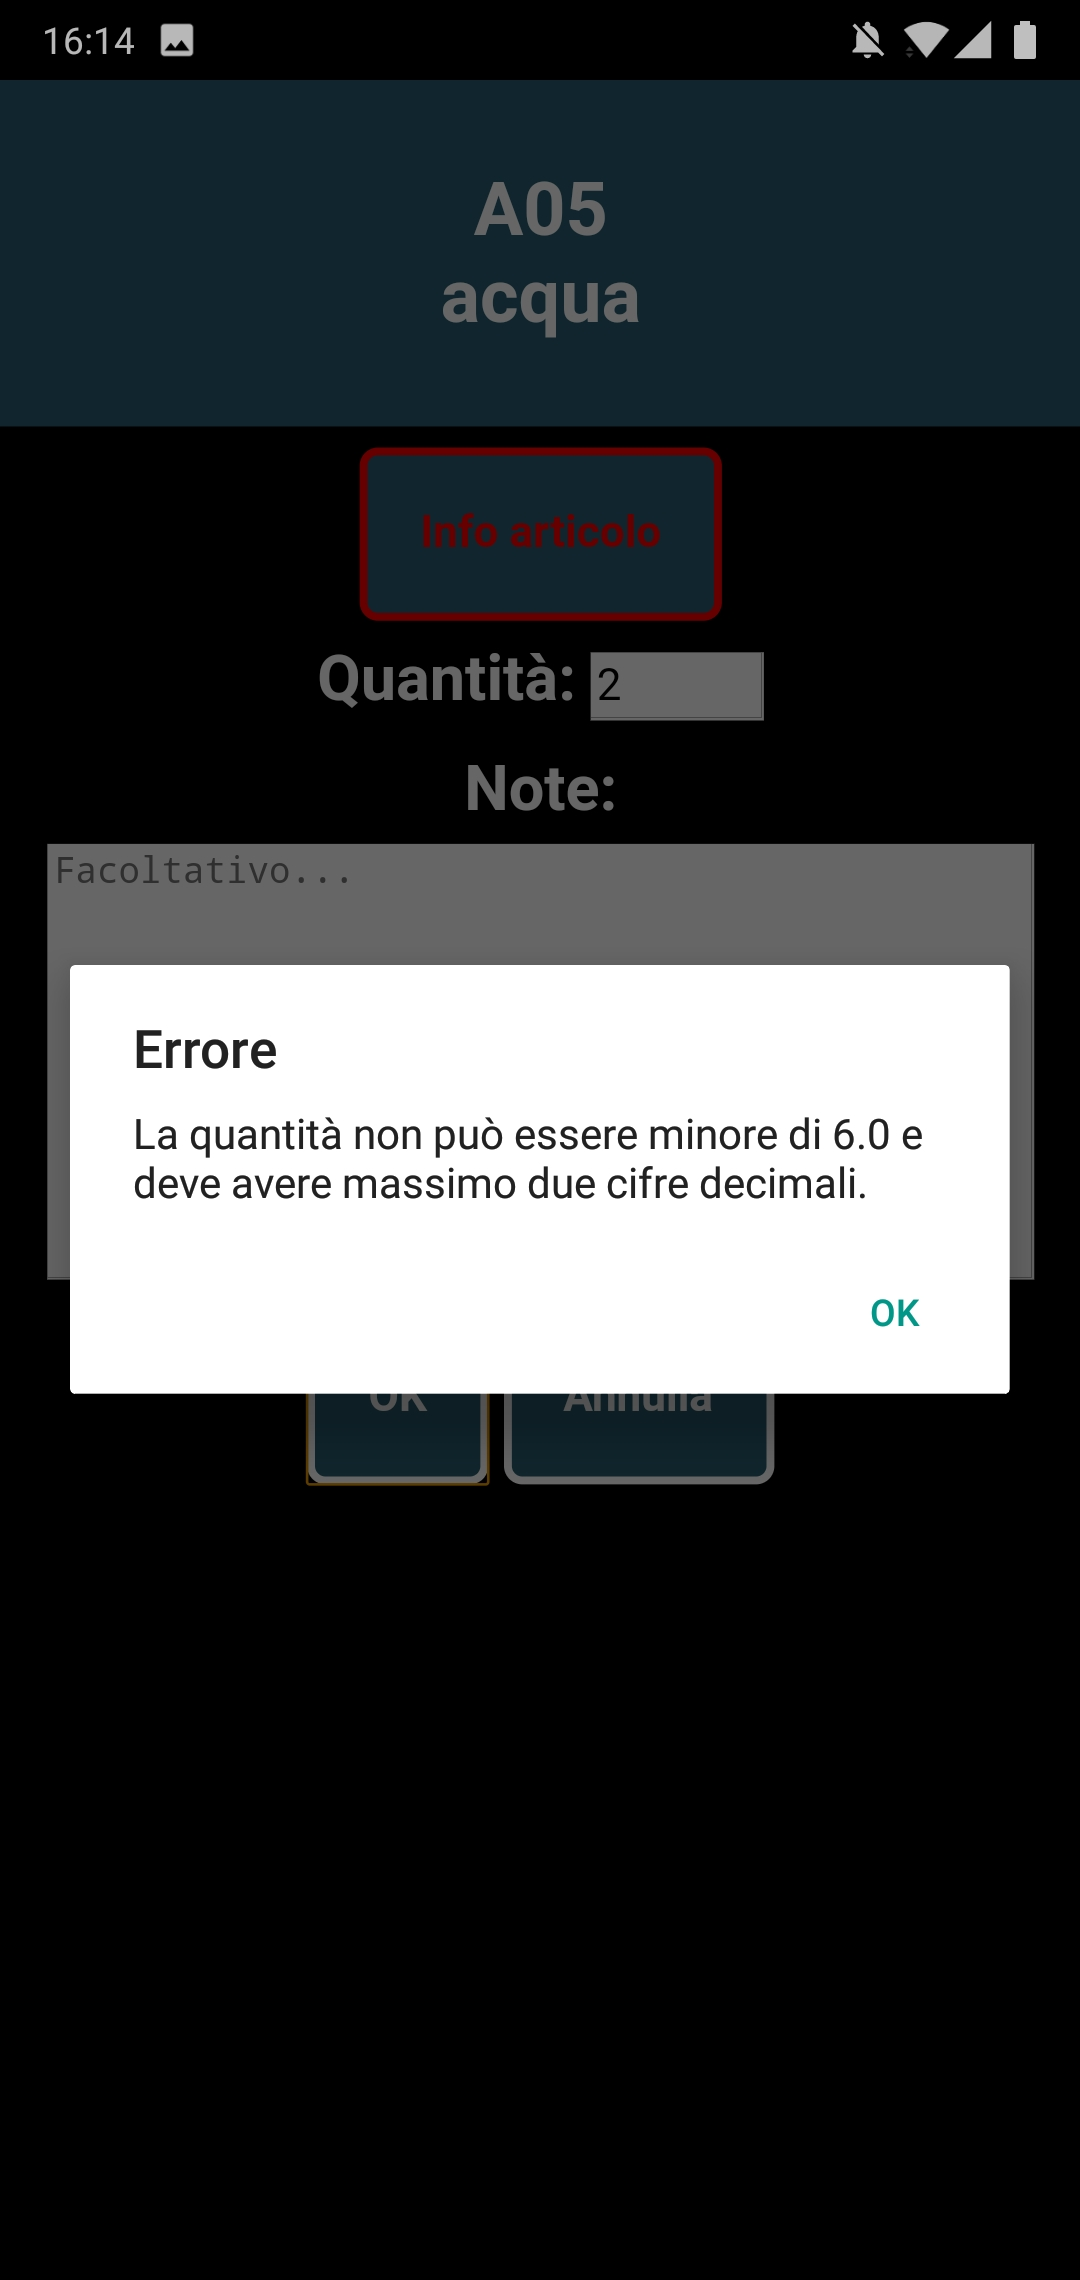
\includegraphics[width=.4\textwidth]{./img/erroreQta2.jpg}
	\caption[Possibili dialog di errata quantità di un articolo]{A sinistra il messaggio lanciato in caso di quantità non inserita; a destra il messaggio lanciato in caso di quantità non valida}
\end{figure}

\newpage

\subsection{Pagina di modifica di un articolo}

La pagina di modifica di un articolo è la stessa pagina per l'inserimento di un articolo, con le seguenti differenze:
\begin{itemize}
	\item La pagina viene aperta con i dati già inseriti precedentemente per l'articolo selezionato;
	\item Premendo sul pulsante ``OK" verrà eseguita la modifica dell'articolo selezionato e non l'inserimento di un nuovo articolo;
	\item Premendo sul pulsante ``Annulla" si tornerà alla home page dell'applicazione e l'articolo precedentemente selezionato per la modifica
	risulterà ancora in carrello con i dati precedentemente inseriti.
\end{itemize}





